% REMEMBER: You must not plagiarise anything in your report. Be extremely careful.

\documentclass{l4proj}

    
%
% put any additional packages here
%



\begin{document}

%==============================================================================
%% METADATA
\title{Talk JSON to me: Exploring natural language descriptions of JSON files}
\author{Holly Hewitt}
\date{March 24, 2023}

\maketitle

%==============================================================================
%% ABSTRACT
\begin{abstract}

In this project, we introduce JSONTalk, a command-line tool that can generate natural language summaries of JSON files. We present a technique using a visitor design pattern to traverse an Abstract Syntax Tree to map syntactic and semantic JSON elements to natual language constructs. The tool we developd has the potential to assist visually impaired, time-constrained, and novice programmers working with JSON data. We evaluated the accuracy and effectiveness of JSONTalk in facilitating the understanding of JSON files, and analysed its usability through a user study. Results of our evaluation of the tool with 40 participants reveal that JSONTalk is a viable alternative to using a screen reader directly with a JSON file, allowing for users to better understand the depth of elements within the JSON file, and decipher the underlying JSON file more quickly and accurately.

Additionally, in this project we reviewed state-of-the-art techniques currently used for code summarisation with the aim of automating documentation workflows, and highlight the potential for using sophisticated techniques to assist visually impaired programmers in gaining an overview of code and structured data. We also identified a set of research questions that could be explored in future work related to the use of generative AI as a code summary tool, and its potential to improve computing accessibility for visually impaired programmers.

\end{abstract}

%==============================================================================

% EDUCATION REUSE CONSENT FORM
% If you consent to your project being shown to future students for educational purposes
% then insert your name and the date below to  sign the education use form that appears in the front of the document. 
% You must explicitly give consent if you wish to do so.
% If you sign, your project may be included in the Hall of Fame if it scores particularly highly.
%
% Please note that you are under no obligation to sign 
% this declaration, but doing so would help future students.
%
\def\consentname {Holly Hewitt} % your full name
\def\consentdate {23 February 2023} % the date you agree
%
\educationalconsent


%==============================================================================
\tableofcontents

%==============================================================================
%% Notes on formatting
%==============================================================================
% The first page, abstract and table of contents are numbered using Roman numerals and are not
% included in the page count. 
%
% From now on pages are numbered
% using Arabic numerals. Therefore, immediately after the first call to \chapter we need the call
% \pagenumbering{arabic} and this should be called once only in the document. 
%
% Do not alter the bibliography style.
%
% The first Chapter should then be on page 1. You are allowed 40 pages for a 40 credit project and 30 pages for a 
% 20 credit report. This includes everything numbered in Arabic numerals (excluding front matter) up
% to but excluding the appendices and bibliography.
%
% You must not alter text size (it is currently 10pt) or alter margins or spacing.
%
%
%==================================================================================================================================
%
% IMPORTANT
% The chapter headings here are **suggestions**. You don't have to follow this model if
% it doesn't fit your project. Every project should have an introduction and conclusion,
% however. 
%
%==================================================================================================================================
\chapter{Introduction}

% reset page numbering. Don't remove this!
\pagenumbering{arabic} 

This project has involved the design, development, and evaluation of JSONTalk. JSONTalk is a command line tool that can generate human-readable, customisable descriptions of JSON files. This chapter provides a brief overview of the motivation for this project, a summary of the JSONTalk features, and summarises our evaluation of JSONTalk. We also conducted an exploratory study on using ChatGPT as an alternative code summarising tool and provide an overview of it in this chapter.

\section{JSON}
To fully understand the motivation for a JSON summarising tool, it is firstly important to know what JSON is. JSON is a widely used text-based data interchange format \cite{JSON}. JSON documents encode primitive data types (Boolean, String, number, null) and two compound data types (objects and arrays). Colons are used to separate key-value pairs, objects are surrounded with curly braces, ‘{}’, and arrays are surrounded with square brackets, ‘[]’.  

JSON files are used in a variety of different areas of computer science. The main categories are as follows: 
\begin{enumerate}
    \item Remote data exchange: JSON is commonly used to exchange data between web servers and clients. For example, JSON is the most common data format used to exchange data in RESTful APIs \cite{Barbaglia_Murzilli_Cudini_2017}.
    \item Software Configuration: JSON can be used to store configuration information for applications.
    \item Event Logging: JSON is a simple, structured solution to store data about events and transactions.
    \item NoSQL databases: MongoDB and CouchDB are two examples of NoSQL databases that store data in JSON format.
    \item Big Data: JSON is used in big data applications for storing and processing large volumes of data. 
\end{enumerate}

As illustrated in the use cases above, programmers and software developers are the people who are most likely to interact with JSON files. This interaction can include the writing of JSON files and the development of a system that involves JSON files, thus having to read JSON files. Although one of the key benefits of JSON is its human-readable text format to represent key value pairs \cite{friesen2019introducing, nurseitov2009comparison, JSON}, it should be noted that this may not be the case for visually impaired (VI) programmers. In reality, visual cues, such as indentation and punctuation, can make JSON files difficult to read and understand for those with visual impairments. Although JSON may offer certain advantages for some developers, it is important to recognise that its benefits may not be universal, and additional accommodations may be necessary to ensure equal access and opportunity for all programmers. To address this accessibility barrier, we have developed JSONTalk, a tool to provide more screen reader-friendly descriptions of JSON documents. 

\section{Challenges faced by visually impaired programmers}

Out of 77,375 developers surveyed in the Stack Overflow May 2021 developer survey \cite{stack22}, only 1.7\% (1,238 respondents) reported being blind or visually impaired. At least 2.2 billion people worldwide suffer from some level of vision loss or impairment \cite{World}. Jobs in computer science and software development have the potential to provide meaningful livelihood opportunities for visually impaired individuals. These professions offer flexible work arrangements, high job growth, and competitive salaries. However, there are still significant accessibility barriers that prevent visually impaired individuals from fully participating in these industries. The challenges faced by VI programmers can be summarised as follows:


\begin{itemize}
    \item \textbf{Harder to skim code}: VI programmers are constrained to using screen reader or braille display to read code line by line, making it harder to quickly understand code structure and relationships.
    \item \textbf{Inaccessibility of code overview diagrams}: UML diagrams, code overview graphs, and trees used in IDEs are often key to gaining a better understanding of code structure; however, these are highly visual and often inaccessible to VI programmers.
    \item \textbf{Debugging discover-ability}: While IDEs offer visual cues like underlined code to help sighted programmers identify issues, VI programmers may not have equivalent nonvisual cues to aid in debugging, making it challenging for them to identify and fix bugs in their code.
    \item \textbf{Missed visual cues}: VI programmers may miss out on visual cues, such as syntax highlighting and indentation, which help sighted programmers write, edit, and read code more efficiently.
    \item \textbf{Limited access to training and resources}: There is a difference in the abundance of tools and resources available for sighted programmers versus those available and accessible for VI programmers. Resources such as block-based programming languages used in the early stages of computer science education are often highly visual and inaccessible.
\end{itemize}


Although there are still significant barriers to accessibility to programming, various tools have been developed to make programming more accessible to VI programmers. These tools can be categorised into three categories: standalone tools, IDE plugins, and programming languages.  The background section of the dissertation will involve an analysis of the some of tools and research aimed to address these accessibilities. 

\begin{itemize}
    \item Accessible standalone tools: JavaSpeak \cite{Javaspeak_2000}, Code Mirror Block \cite{code_mirror_block_2019}, ACONT \cite{ACONT_2018}, BridgIT \cite{BridgIT_2011}, Blocks4All\cite{blocks4all_17, blocks4all_18}, Noodle\cite{Noodle_2014}, CodeMirrorBlocks \cite{code_mirror_block_2019}, Myna \cite{Myna}
    \item Accessible IDE plugins: Aural Tree Navigator \cite{aural_tree_navigator_2003}, StructJumper \cite{structujumper_2015}, AudioHighlight \cite{audiohighlight_2018}, Tactile Code Skimmer \cite{tactile_code_skimmer_2019}, CodeTalk \cite{codetalk_18}, Wicked Audio Debugger \cite{Wicked_audio_debugger_2007}, SODBeans \cite{Sodbeans_2009}, Accessible version of Blockly \cite{Blockly1_2017}
    \item Accessible programming languages: GUIDL \cite{GUIDL_2012}, Quorum \cite{Quorum_2017}, Pseodospatial Blocks \cite{Pseudospatial_blocks_2016}, Audio Programming Language (APL) \cite{Audio_programming_language_2006}
\end{itemize}

The above bullet points provide a comprehensive overview of the tools available to VI programmers. In the background section we will not explore all of these tools. Instead we have selected the most relevant subset of these tools and critically analysed them.

\section{JSONTalk}

\begin{figure}
    \centering
    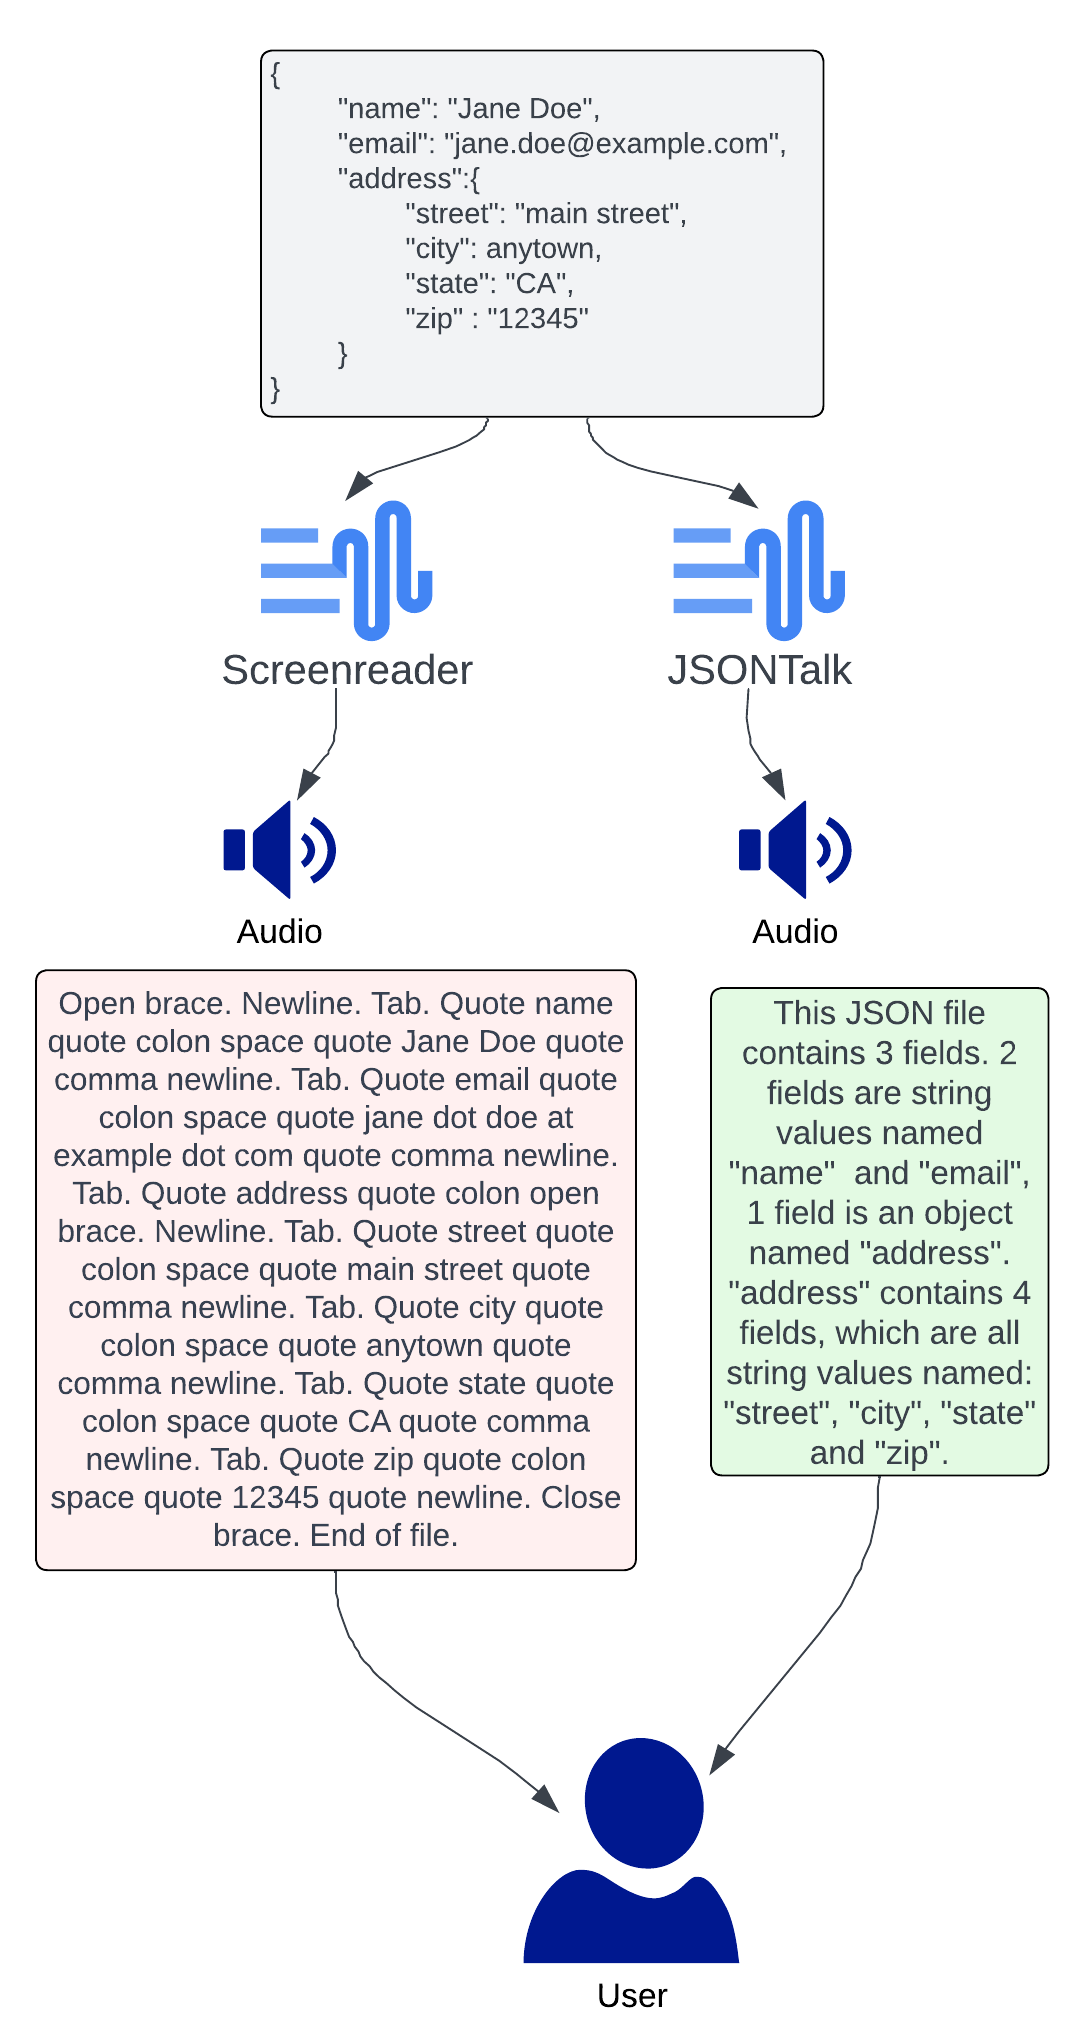
\includegraphics[width=0.7\textwidth]{dissertation/images/JSONTalk updated.png}
    \caption{Using JSONTalk vs using a screen reader }
    \label{fig:JSONTalk_use_case}
\end{figure}


To primarily supplement missed syntactic visual cues and address the code skimming challenges faced by VI programmers, we developed JSONTalk. Whilst there has been significant work towards creating accessible IDEs, IDE plugins and programming languages, there is no tool that helps VI programmers to read and understand the contents and structure of JSON files. JSONTalk is a command line tool that takes a JSON file and generates a variety of screen reader-friendly descriptions of the file. JSON files are often long and repetitive in nature, and it is not necessary for programmers to read JSON documents line by line, as often understanding the overall structure of the file is enough for programmers to be able to work with the file.

JSONTalk can generate several different descriptions. 
\begin{itemize}
    \item Top-level overview of the file
    \item Structural overview of the different complex elements that make up the file (objects and arrays)
    \item In depth detailed description of the file, including keys and values
\end{itemize}

In addition to the 3 different levels of description that users can request from the tool, there are an additional two parameters that can be set by the user to customise the descriptions detailed above:
\begin{itemize}
    \item Users can set the depth of the description, i.e. only key-value pairs up to depth 3 will be read out, which generates a shorter description for users 
    \item Users can also turn on a nesting option that explicitly reads out the nesting depth of each object or array. This helps users understand the context of the code and makes reading the file less visually demanding. This option is essentially an audio equivalent of indentation.
\end{itemize}

\section{Evaluation of JSONTalk}

We conducted a user evaluation to evaluate the effectiveness and usability of the JSONTalk tool in representing JSON files for screen reader users. A between-subjects A/B testing design was used, where participants answered questions related to three different JSON file screen reader transcripts with or without the JSONTalk tool. The evaluation collected data on error rates, similarity between the rewritten and actual JSON files, time taken to complete tasks, and user feedback on the tool's usability. While the evaluation involved sighted programmers, the use of screen reader transcripts ensured a more realistic representation of the tool's use case. The evaluation results were analysed to answer research questions related to the accuracy of JSONTalk, its effectiveness in facilitating the understanding of JSON files, and its usability. 

In our study, we found that JSONTalk allows users to better understand the depth of elements within JSON files. This feature is especially useful for VI programmers who cannot rely on visual cues, such as indentation, to convey the depth of elements. We also found that the tool allows users to decipher the represented JSON file more quickly and accurately, compared to when using a screen reader.

\section{Exploratory study of ChatGPT}

With the rise in popularity of generative AI, we conducted an exploratory study to determine the feasibility of using a generative AI tool for the generation of natural language descriptions for JSON data. ChatGPT \cite{chatgpt} was released by OpenAI in November 2022. ChatGPT is a large language model developed by OpenAI, based on the GPT-3.5 architecture, trained to generate human-like responses to queries in natural language. It uses machine learning algorithms to understand and respond to a wide range of topics, making it a versatile tool for various applications.

In our study, we asked ChatGPT to describe three different JSON files, with the same prompt each time. We analysed each response, and recorded the observations made, comparing the descriptions generated by ChatGPT to the descriptions generated by JSONTalk.

%==================================================================================================================================
\chapter{Background}

The background section of this dissertation will delve into the challenges faced by VI programmers and the tools developed to make programming more accessible for them. The section will analyse the different categories of tools developed, including standalone tools, IDE plugins, and accessible programming languages.

\section{Assistive technology to aid VI computer users}

This sub-section provides an overview of the assistive technology commonly used by VI computer users generally. There is a diverse range of tools available for VI programmers, although it is important to note that some of them are more accessible than others in terms of cost. Additionally, funding available for the purchase of essential assistive technology is often limited \cite{assistive_tech_funding}. Please note that this subsection does not cover tools specifically developed for programming tasks; tools specifically developed for programming tasks will be covered in a later subsection. 

\subsection{Assistive technology overview}
Screen readers are a vital accessibility tool that enables individuals with visual impairments to navigate digital content. They are particularly helpful for users who have significant visual impairments and need to rely on auditory signals to access information. Screen readers use a combination of text-to-speech and keyboard commands to read out text on a computer screen. They can also provide audio descriptions of images, videos, and other visual elements, allowing users to fully understand the content. Moreover, screen readers are not limited to just desktop computers or laptops, they can also be used on mobile devices, making digital content accessible on-the-go.

Another type of aid that can be particularly helpful for VI computer users are Braille output devices (also named refreshable braille displays); see Figure \ref{fig:braille display}, which convert on-screen text to Braille, allowing users to read the text with their fingers. These hardware devices use an array of pins to display Braille characters that correspond to the on-screen text. Braille output devices are particularly useful for users who are blind or have significant visual impairments and rely on tactile cues to access information. They allow users to read text, navigate menus, and perform other computer functions with touch. Additionally, Braille output devices can be used in conjunction with screen readers, providing users with multiple ways to access and interact with digital content. 

\begin{wrapfigure}{R}{0.5\textwidth}
    \centering
    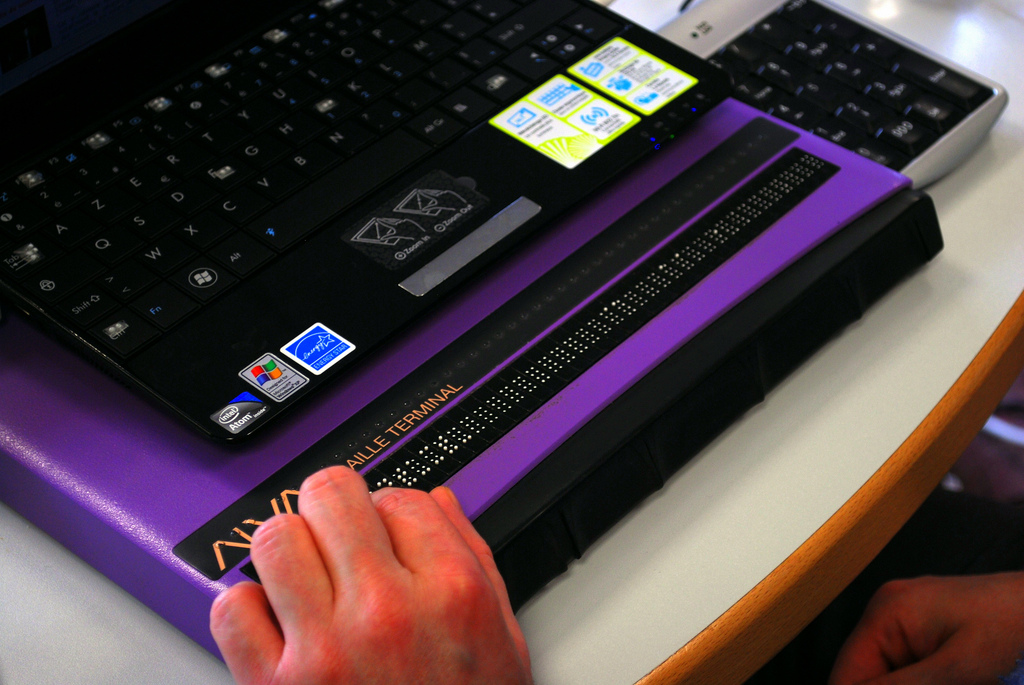
\includegraphics[width=0.5\textwidth]{dissertation/images/Plage-braille.jpg}
    \caption{40 cell refresh-able braille display \cite{braille}}
    \label{fig:braille display}
\end{wrapfigure}

Magnification software is another aid that can be particularly helpful for VI computer users. This type of software zooms in on the screen, making text and other elements larger and easier to see. This can be particularly helpful for users who have low vision and need to increase the size of text and other elements to access them. It is important to note that magnification software may not be suitable for users with severe visual impairments or those who are completely blind. In such cases, screen readers or Braille output devices may be more suitable. 

High contrast or colour-inversion themes are another type of aid that can be particularly useful for users with low vision. These are themes that adjust the colour scheme of the user interface to make it high contrast, making it easier to distinguish between different elements. This can be particularly helpful for users who have difficulty distinguishing between different colours or who have low contrast sensitivity. Again, this aid will only benefit users who have less severe levels of visual impairment.

Magnification software, high contrast and colour inversion themes are often packaged together in a tool to simplify the accessibility process for users, as they can access all of the necessary features in one place without having to navigate multiple settings. When developing tools for VI users, it is crucial to note that visual impairment is a wide spectrum \cite{WHO_2021}. Customise-ability is an essential aspect of assistive technology for VI users \cite{keates2003countering}, as it allows them to tailor the technology to their specific needs and preferences, making it easier for them to access and interact with digital content. 

Finally, speech recognition software is another aid that can be helpful for VI computer users. This type of software allows users to control their computer using voice commands, which is particularly helpful for users who have physical disabilities or who cannot use a mouse or keyboard. However, the need for audio input is not as strong as the need for audio or tactile output. Most VI users are able to type \cite{miele2017assistive}, having memorised the layout of a keyboard. Whilst speech to text software is still useful for some VI users, this dissertation will focus on providing accessible output to help VI users understand code.




\subsection{The challenges of coding with a screen reader or braille-display}

%\begin{figure}
 %   \centering
 %   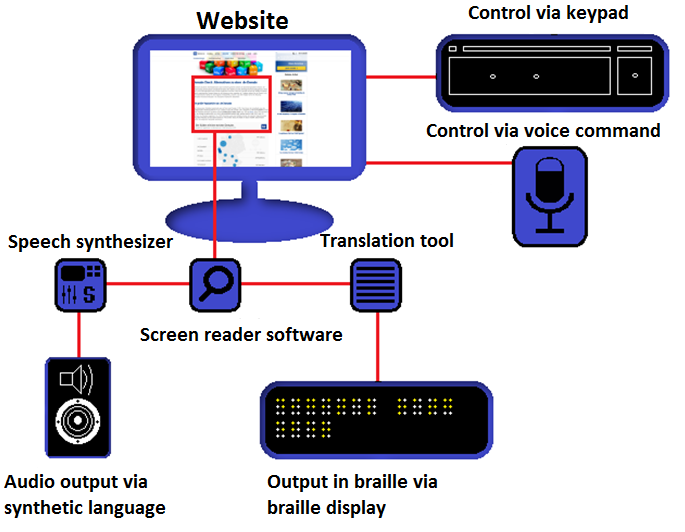
\includegraphics[width=0.9\textwidth]{dissertation/images/EN-Screenreader.png}
 %   \caption{Diagram illustrating web access using accessibility aids\cite{EN-Screenreader}}
 %   \label{fig:screen reader}
%\end{figure}

This section will discuss the challenges faced by VI programmers. In recent years, there has been growing attention to the challenges faced by VI programmers, and significant progress has been made in research to understand and address these challenges. We will focus on the challenges faced by programmers with severe levels of visual impairment who use screen readers and refreshable braille displays.
\paragraph{Challenges associated with using screen readers and braille displays:}
\begin{itemize}
\item \textbf{Limited to reading code sequentially (line by line):}  \cite{code_mirror_block_2019} A consequence of this is lower levels of code comprehension \cite{ Mountapmbeme_Okafor_Ludi_2022}. The limitation of reading code sequentially creates further challenges for VI programmers. 
\begin{itemize}
\item  \textbf{Harder to skim code}: Being constrained to reading code line by line makes VI programmers unable to “skim” code in the same way that sighted programmers can. Code skimming is a useful way for users to get a quick overview of the main functionality of code without getting bogged down by the details. screen readers and braille displays do not offer any method for VI programmers to effectively skim code. The consequences of this are increased time required to read over code, and lower levels of code comprehension. \cite{structujumper_2015}
\item \textbf{Harder to back-track}: When using screen readers and braille displays, it can be challenging for programmers to navigate back to the part of code they were previously focused on. Sight allows programmers to easily identify and correct errors, but for VI programmers using accessibility tools, this process can be much more difficult \cite{Javaspeak_2000}.
\item \textbf{Harder to understand structure of code represented through visual cues}: Many programming languages use visual cues such as indentation and white space to indicate the structure of the code. VI programmers who use screen readers or braille displays may struggle to perceive these visual cues, making it more difficult to understand the structure of code. \cite{code_mirror_block_2019} 
\item \textbf{Harder to find information within a code base without losing the position of focus}: VI programmers have reported challenges related to moving around different parts of code without losing previous focus \cite{ Albusays_Ludi_2016}. 
	\end{itemize}

\item \textbf{Limited access to visual information}: Visual information such as diagrams, charts, and graphs can be difficult for screen readers to interpret, which can be a barrier to VI programmers who need to work with this type of information. Awareness of bugs within code is often raised using visual cues, such as squiggly red lines underneath problems. screen readers and braille readers often cannot represent visual information pertaining to code or visual cues pertaining to bugs within code. This leads to lower levels of code comprehension amongst VI programmers, and higher numbers of bugs within code produced by VI programmers. 

\item \textbf{Incompatible graphical user interfaces}: Graphical user interfaces, such as IDEs (see Figure \ref{fig:ide}), are commonly used by sighted software developers to speed up the development process. Often there is a lack of compatibility between screen reader or braille display software and the graphical elements of these tools \cite{GUIDL_2012}. This puts VI programmers at a significant productivity disadvantage compared to their sighted colleagues, who have unhindered access to productivity boosting features of IDEs \cite{ Mountapmbeme_Okafor_Ludi_2022} and other GUI based tools, such as block-based programming languages such as Scratch \cite{scratch}. Whilst these tools have brought great benefit to the software development and computer science education community, it is important to recognise that the development of GUI based software development and educational tools has increased the accessibility gap between sighted and VI developers. \cite{code_mirror_block_2019}


%\begin{figure}
  % \centering
  %  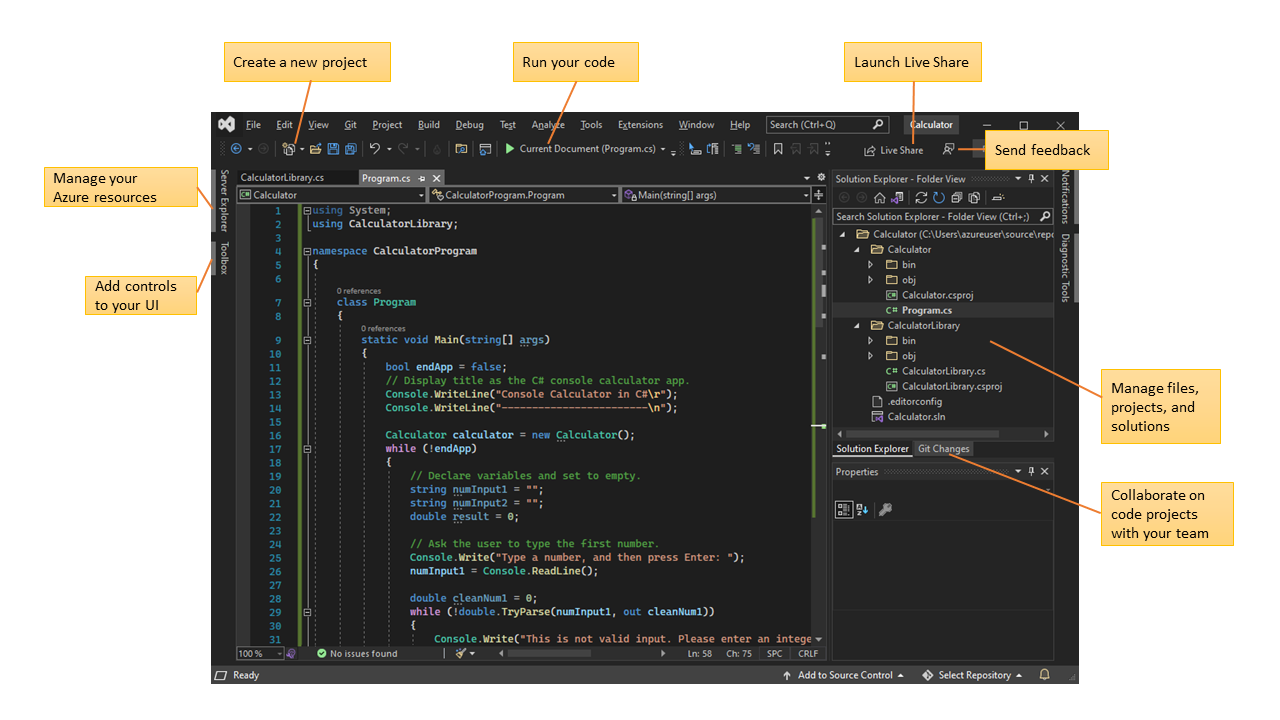
\includegraphics[width=1.2\textwidth, center]{dissertation/images/ide-overview.png}
  %  \caption{Visual Studio IDE Graphical User Interface \cite{ide-overview}}
  %  \label{fig:ide}
%\end{figure}

\item \textbf{Web accessibility}: The web provides many resources to aid programmers in learning computer science concepts, debugging help, and important software documentation. According to the WebAIM Million report \cite{webAIM}, which analysed the top 1 million web home pages in 2021, only about 2.4\% of the home pages met the Web Content Accessibility Guidelines (WCAG) 2.0 Level AA accessibility standards, meaning that the majority of web pages have accessibility issues to some extent.

\item \textbf{Harder to edit code without losing focus}: VI programmers have reported issues surrounding virtual cursor control when editing code. It can be difficult to edit the code in place and return to the original point of focus with the cursor \cite{Mealin_Murphy-Hill_2012}. Workarounds such as copying code, editing it separately, and pasting it back in are employed by some VI programmers. This is more time-consuming than that simple in-place coding editing that can be done by sighted programmers. 
\end{itemize}


\paragraph{Challenges specific to screen readers:}
\begin{itemize}
\item \textbf{Time}: Screen readers can read large amounts of code aloud, but the time taken to listen to this code can be much longer than the time it would take for a sighted programmer to read the same code. This can be a significant issue, as programmers often need to read and understand large amounts of code in a short period of time. Screen readers typically have settings to adjust the speaking speed, but increasing the speed too much can make it difficult to understand the code being spoken. Punctuation is a vital element in the syntactic nature of code, whilst this can be represented by a single character which can be quickly read and understood in text or braille format, screen readers deal with punctuation in one of two ways. The first way is skipping over punctuation, when this is done the user may miss out on vital information about the program code and lead to a lower level of code comprehension. The alternative is to explicitly read out punctuation. This method is time-consuming, and putting too much emphasis on punctuation may cloud the users focus, leading to lower levels of code comprehension. 

\item \textbf{Consistency}: Different screen readers may have different ways of presenting information and navigating code, which can make it difficult for VI programmers to switch between platforms or collaborate with sighted colleagues.
\end{itemize}


\paragraph{Challenges specific to braille displays:}
\begin{itemize}
\item \textbf{Price}: Braille displays can be much more expensive than traditional displays, making them less accessible to VI programmers who may not have the resources to purchase them.

\item \textbf{Size}: Braille displays can range in size from portable devices with 14-20 cells to larger desktop models with 40-80 cells. Each cell can represents a character. The ideal braille display for a programmer would be 80 cells; however, larger sizes of braille display come at a much higher cost. Developers using smaller displays may need to read one line of code in multiple lines of braille. Additionally, this may also be the case for users of 80 cell braille displays. Whilst 80 characters per line is accepted as a standard for many programming languages \cite{Characters_per_line} it is often not enforced. This means that reading code that does not comply with this standard will pose a challenge for all braille display users, regardless of the size of their braille display.
\end{itemize}


\section{Tools created specifically for VI programmers}
\label{section: VI_tools}

\subsection{Tool overview}

In the introduction, we categorised the tools available for visually impaired programmers as standalone tools, IDE plugins and accessible programming languages. We will use the same categories here.

\subsubsection{Standalone tools:}

JavaSpeak \cite{Javaspeak_2000} is a programming tool designed to assist students with visual disabilities in learning to code in Java. The tool is built with a keyboard and speech interface, making it fully usable for users with visual impairments. Its main feature is providing aural feedback, allowing users to comprehend a program's structure and semantics. The software works by analysing the program's code and speaking its structure to the user. 

CodeMirrorBlocks \cite{code_mirror_block_2019} is a browser-based, language-independent tool for creating fully accessible, block-based programming environments for visually-impaired programmers. It uses an extensible system that can run on web browsers without requiring any plugins or extra programs to be installed. The tool communicates the structure of the code using spoken descriptions and allows for navigation using standard keyboard shortcuts. CodeMirrorBlocks creates block-based representations of code from Abstract Syntax Trees (ASTs) with descriptive labels to give users more context about the location and depth of the line of code they are hearing or looking at. This approach helps VI users to orient themselves and 'skim' code in a way that their prior resources such as screen readers and IDEs had not allowed. The tool is performant, responsive, and memory efficient enough to run on tablets, under-powered laptops, etc.

The paper "An Empirical Evaluation of a Vocal User Interface for Programming by Voice" \cite{Myna} discusses the challenges of mapping a graphical user interface (GUI) to a Vocal User Interface (VUI) for individuals with physical disabilities who may struggle to use a mouse and keyboard. The paper focuses on Myna, a VUI mapped to the Scratch programming environment, and presents initial user studies on its effectiveness. The paper emphasises the importance of designing applications that adapt to user needs rather than the other way around, and discusses the challenges of creating a VUI for an application whose GUI changes dynamically. The paper concludes that there was no significant time difference between GUI and VUI use and that the added functionality that vocal input provides outweighs the small increase in time, particularly for motor-challenged individuals who cannot use GUI-based interfaces. However, the paper notes that strong vocal articulation skills and stamina are required for users to effectively use a VUI.

\subsubsection{IDE Plugins:}

AudioHighlight \cite{audiohighlight_2018} is a software tool designed to improve the experience of VI programmers when reading and navigating through code. VI programmers typically rely on screen readers to read the code aloud, but this process can be slow and tedious since screen readers read every word and character sequentially. AudioHighlight addresses this issue by rendering code inside a web view, which allows it to place HTML heading tags on the structural elements of the source code, such as classes, functions, and control flow statements.
The tool leverages the familiar interface of web pages and virtual cursors used by screen readers to navigate structural information such as HTML heading tags. This approach allows VI programmers to skim through the code and quickly identify the most important areas of the code. The tool can be used as a web service or as part of the Eclipse Integrated Development Environment (IDE).
AudioHighlight was compared to two other approaches, StructJumper and GitHub, and was found to be superior in terms of both speed and quality of code comprehension. The software allows VI programmers to skim code on the web without the need to import it into an IDE, making it a more accessible and efficient solution for VI programmers. Overall, AudioHighlight is a powerful tool for improving the accessibility of code for VI programmers, enabling them to navigate and comprehend code more efficiently.

StructJumper \cite{structujumper_2015} is an Eclipse plugin designed to assist VI programmers in navigating and understanding the structure of Java code. The tool creates a hierarchical tree based on the nesting structure of a Java class, allowing programmers to get an overview of the code structure, including all the methods and control flow statements. The programmer can quickly switch between the TreeView and the Text Editor to get an idea of where they are within the nested structure. The paper evaluated the tool with seven VI programmers that completed three tasks with and without the tool and found that users completed tasks faster with StructJumper. The tool addresses the accessibility issue faced by VI programmers to understand the overall structure of a Java class and provides a more efficient way for them to navigate and understand the code. The paper also highlights the importance of encapsulating all information within the same view, as this approach can enhance the accessibility of the code for VI programmers.

CodeTalk \cite{codetalk_18} is a Visual Studio plugin designed to improve accessibility for VI programmers by addressing the accessibility challenges faced by them in using Graphical User Interface (GUI) based programming environments. The paper categorises the accessibility difficulties into four categories, namely Discoverability, Glanceability, Navigability, and Alertability, based on a survey of VI developers and the authors' personal experiences. CodeTalk extracts useful visual information presented by IDEs and provides it in multiple audio channels to the developer. The tool provides a code summary and functions list, code context information, real-time error information, and audio debugging. The authors evaluated the tool by measuring and comparing performance metrics with and without tool use, as well as an online survey, which received positive user feedback.

\subsubsection{Accessible programming languages:} 

The Graphical User Interface Description Language (GUIDL) \cite{GUIDL_2012} is a new approach to visual programming for people with visual disabilities. VI programmers have faced challenges with traditional visual user interfaces, especially in desktop programming. Although some efforts have been made to help people with visual impairment work with graphical interfaces, none have provided a fully usable solution for VI programming professionals. In this paper, different approaches are discussed and a proposed solution is presented in the form of GUIDL. GUIDL is a new system that includes a description language that enables VI programmers to create graphical interfaces as part of their programs. This new system would be acceptable to not only professional programmers but also to designers and other VI computer hobbyists. The proposed system is based on the initial ideas and research results obtained by studying the needs of VI programmers. The paper provides a formal description of the proposed system, with a focus on the description language as its core component. In summary, GUIDL is an innovative approach that has the potential to revolutionise visual programming for people with visual impairments.

\subsubsection{Related research:}

The paper "ACONT: An Initial Investigation into Nonvisual Code Structure Overview Through Speech, Non-speech and Spearcons" \cite{ACONT_2018} investigates non-visual methods to provide an overview of object-oriented source code for visually-impaired programmers. A user study of ten sighted and three nonsighted participants compared the effectiveness of speech, non-speech, and spearcons for quickly overviewing a class file. Speech cues were found to be more effective than non-speech and spearcons in identifying programming constructs and answering questions. However, some positive feedback was received for non-speech outputs, indicating potential for further exploration. The paper highlights the benefits of nonvisual methods for code structure overview and suggests further research to explore non-speech cues and optimal design choices.

Stefik et al. present an empirical investigation into the design of auditory signals to improve the comprehension of computer programmes \cite{Stefik_Hundhausen_Patterson_2011}. The research compares the comprehensibility of two alternative auditory program representations, one with lexical scoping cues and another without, using a novel approach called artefact encoding. The study also compares programmers' ability to debug programs using three alternative environments: an auditory execution environment with the empirically derived auditory cues, an auditory execution environment with the current state-of-the-art auditory cues generated by a screen reader running on top of Microsoft Visual Studio, and a visual version of the execution environment. The results of the study showed that well-designed auditory cues can make a significant difference in program comprehension for programmers with vision impairments or sighted people. The research contributes a novel methodology and foundational empirical data that can guide the design of effective auditory representations of computer programs. The paper also discusses concepts such as semantic priming and temporal masking that may affect the effectiveness of auditory cues.

\subsection{Critical analysis of the tools}
The selected tools aim to improve the accessibility and inclusion of programming for people with disabilities. JavaSpeak and CodeMirrorBlocks provide an aural interface for people with visual impairments, while GUIDL and Myna provide solutions for programming with graphical user interfaces through description languages and vocal user interfaces. AudioHighlight and StructJumper address the issue of code comprehension, enabling VI programmers to navigate and understand the structure of code. CodeTalk is a Visual Studio plugin designed for people with visual impairments that uses spoken natural language to navigate and write code.

JavaSpeak and CodeMirrorBlocks are both designed for users with visual impairments, providing a more accessible and inclusive learning experience. JavaSpeak uses a keyboard and speech interface, providing aural feedback to comprehend the structure and semantics of the code. CodeMirrorBlocks creates block-based representations of code, with descriptive labels providing users with more context about the location and depth of the code they are hearing or looking at.

GUIDL and Myna enable VI programmers to program with graphical user interfaces. GUIDL provides a new system that includes a description language to create graphical interfaces as part of programs. Myna is a vocal user interface mapped to the Scratch programming environment that allows individuals with physical disabilities who may struggle to use a mouse and keyboard to program.

AudioHighlight and StructJumper address the issue of code comprehension for VI programmers. AudioHighlight places HTML heading tags on the structural elements of the code, allowing screen readers to skim through the code and quickly identify the most important areas of the code. StructJumper creates a hierarchical tree based on the nesting structure of a Java class, providing an overview of the code structure and a more efficient way to navigate and understand the code.

CodeTalk is a Visual Studio plugin designed for people with visual impairments that uses spoken natural language to navigate and write code. It provides a more accessible and efficient solution for people with visual impairments to program.

These tools are a significant contribution towards creating an inclusive and accessible programming environment for all.

\section{Code and structured text summarising: State-of-the-art}

This section explores various techniques and tools used for summarising code and structured text such as JSON, XML, and YAML. Some of the tools designed to assist VI programmers, discussed in section \ref{section: VI_tools}, use summarisation to overcome code overview accessibility challenges in terms of code overview and comprehension. t's important to note that the techniques and tools discussed in this section are not exclusively developed for VI programmers. Instead, they are primarily created to automate code documentation workflows and offer all programmers, irrespective of their visual ability, an improved understanding of code and structured text formats used within software development.

\subsection{Code summarisation techniques and tools}
\label{section:code_summary}

Information retrieval techniques are commonly used to extract useful information from source code to automatically generate natural language descriptions. Various approaches have been proposed using keyword identification, including those by Salton et al. \cite{salton1975vector}, Blei et al. \cite{blei2003latent}, Landauer et al. \cite{landauer1998introduction}, and Haiduc et al. \cite{haiduc2010supporting}. Eye tracking techniques have revealed that developers spend more time reading method signatures than method invocations \cite{rodeghero2014improving}, this finding helped to focus code summarisation efforts. Topic modelling techniques, such as hierarchical panchinko allocation (hPAM)\cite{mimno2007mixtures}, have also been used to generate code summarisations. Static analysis techniques, such as those proposed by Rastkar \cite{rastkar2010summarizing} and Dawood et al. \cite{dawood2017source}, have also been explored. Dawood et al. converted Java code to ASTs and generated a description using for each node visited. 

Researchers have used various techniques to identify abstractions of method function, such as stereotypes and micropatterns. JSummariser is a tool that identified stereotypes within classes and defined different text templates for summarising different stereotypes \cite{moreno2013automatic,abid2015using}. Micropatterns, on the other hand, are abstractions of a method's function, and a method can be mapped to several micropatterns \cite{malhotra2018class,rai2017method}. To generate comments for code segments, Wong et al. crawled code segments together with their descriptions from StackOverflow to automatically generate comments \cite{wong2013autocomment}. Other researchers have used natural language processing techniques to analyse existing code repositories and identified similar code within external repositories to generate comments \cite{wong2015clocom}. Badihi and Heydarnoori proposed gamified crowd-sourcing of code description mappings in their Crowdsummarizer tool \cite{badihi2017crowdsummarizer}, while Huang et al. mined commit-comment pairs from version control systems to generate comments \cite{huang2017mining}.

Natural language processing techniques have also been applied, such as the use of a software word usage model (SWUM) to capture the relationships between words within the code \cite{xia2017measuring}, and the use of the PageRank algorithm to retrieve the most important methods \cite{mcburney2014automatic}, have also been applied. Wang et al. \cite{wang2017automatically} used an AST and operations performed on related objects to identify unit of action related to the object in the method.

In recent years, machine learning and artificial neural networks have been increasingly applied to software engineering tasks, including source code summarisation. These approaches can be categorised as either supervised or unsupervised learning. Supervised learning algorithms, such as support vector machines and Naive Bayes, have been used to rank descriptive sentences \cite{rastkar2013code} and summarise fragments of source code \cite{nazar2016source}. Unsupervised learning algorithms, such as TASSAL \cite{fowkes2017autofolding}, CODE-NN \cite{iyer2016summarizing}, DeppCom \cite{hu2018deep}, Code Attention \cite{zheng2017code}, and Convolutional Attention Network \cite{allamanis2016convolutional}, use various techniques such as RNNs, LSTM, and attention mechanisms to generate natural language comments summarising source code. These models have been shown to outperform traditional approaches such as keyword identification and static analysis. For example, DeppCom outperforms CODE-NN \cite{hu2018deep}, and the Convolutional Attention Network generates extremely concise summarisations of code \cite{allamanis2016convolutional}. Overall, the use of machine learning and artificial neural networks shows great promise in automating the task of generating natural language descriptions for source code.


The primary aim of the efforts detailed above has been to facilitate the automatic generation of code comments and commit messages. Well-documented code benefits all programmers, regardless of their visual abilities. These techniques could be further leveraged to assist the development of tools that aim to assist VI programmers. Textual summaries of code are accessible by assistive technology, and the use of sophisticated summary techniques could help further bridge the accessibility gap that VI programmers face in terms of code comprehension and overview challenges. The tools described in Section \ref{section: VI_tools} make use of some information retrieval techniques such as static analysis of code and parsing of tree structures; however, the opportunities presented by machine learning and artificial neural network techniques have not yet been explored in great detail when developing tools for VI programmers.  

\subsection{Structured text summarisation tools and techniques}

The subsection above illustrates how natural language descriptions and summaries of code have been extensively researched. Comparatively less work has been done on generating descriptions and summaries for structured text and data formats like JSON and YAML. Structured data formats, such as JSON, XML, and YAML, are crucial components of modern software development that facilitate efficient data storage, transfer, and manipulation across different systems and applications. Therefore, the development of natural language descriptions and summaries for structured data formats such as JSON, XML, and YAML is a valuable area of research that has the potential to improve the accessibility and usability of these formats for all programmers, including those with disabilities.

Whilst JSON does not allow for commenting, both XML and YAML allow for commenting, thus summarisation could allow for automatic comment generation, and assisting programmers working with files in these formats. Clear, meaningful descriptions of these data formats can also assist VI users who use screen readers or braille displays. 

The JSON, XML, and YAML data formats are generally less flexible than standard programming languages, thus the techniques detailed in section \ref{section:code_summary} could be used to generate summaries.


%==================================================================================================================================
\chapter{Analysis/Requirements}

\section{User analysis}

This section discusses the steps we took at the beginning of the project to consider the potential end users of a tool that would generate descriptions of JSON data and the use cases that would most likely benefit these users.

\label{subsection: personas}
\subsection{User personas}
To ensure that the JSONTalk tool would meet the needs of a diverse user base, we developed user personas to capture the potential end users of a tool that generates descriptions of JSON files. We first decided which type of user interacts with JSON documents. As JSON is a commonly used data exchange format, used primarily for web application data transmission, we were able to narrow down the user persona group to programmers. We then began to consider the different types of programmer who may interact with JSON and their goals and needs. These user personas included the following: 

\begin{itemize}
    \item The VI programmer: This user persona requires a tool that can be easily navigated and read aloud by screen readers. They may also need the ability to customise the tool's font size and colour contrast to ensure legibility. 
    \item The time-constrained programmer: This user persona values a tool that can quickly generate human-readable descriptions of JSON files, saving them time and effort. They may not have the luxury of spending extensive time manually parsing JSON files and need a tool that can do this quickly and efficiently. 
    \item The novice programmer: This user persona needs a tool that can provide clear and concise descriptions of JSON files, using simple and commonly used vocabulary. They may be less familiar with the jargon and technical terms used in JSON file descriptions, making it more difficult for them to understand and work with these files. 
\end{itemize}

By developing these user personas, we gained a deeper understanding of the diverse needs and goals of potential users of the JSONTalk tool. The VI programmer requires a tool that can be easily navigated and read aloud by screen readers, as well as the ability to customise the tool's font size and colour contrast. The time-constrained programmer values a tool that can quickly generate human-readable descriptions of JSON files, saving them time and effort. The novice programmer needs a tool that can provide clear and concise descriptions of JSON files, using simple and commonly used vocabulary. By keeping these different user needs in mind, we were able to design the JSONTalk tool to be more inclusive and accessible to a wider range of users, while still meeting the specific needs of each persona. 

\subsection{User stories}

To guide the design of the tool, a set of user stories was developed to capture the needs and goals of potential users. These user stories provided valuable insights into the ways in which the tool could be used and the features that would be most important to its users. The user stories were used to inform the development of the tool's functionality and user interface, ensuring that the tool was tailored to the needs of its intended users. These user stories were then developed into specific scenarios that would serve as a useful testing framework later in the development life cycle. We categorised the user stories by the user personas created prior.

\begin{small}




\begin{multicols}{2}
\textbf{User persona 1: VI programmer}

\textit{User 1 story 1:}
\begin{itemize}
\item As a VI programmer that uses a screen reader
\item I want a tool that is compatible with screen readers
\item So that I can easily navigate and understand JSON files
\end{itemize}
\columnbreak

\textit{Acceptance criteria}
\begin{itemize}
\item Given a JSON file
\item When a VI user requests a description of the file from the tool using screen reader technologies to assist them
\item Then the user should be able to easily navigate and understand the tool, including tool documentation, and access the desired description without encountering any errors or confusion.
\end{itemize}

\end{multicols}

\begin{multicols}{2}

\textit{User 1 story 2:}
\begin{itemize}
\item As a VI programmer
\item I want a tool that can provide a quick and accurate overview of the structure of a JSON file
\item So that I can efficiently navigate and understand the file with my screen reader.
\end{itemize}
\columnbreak

\textit{Acceptance criteria}
\begin{itemize}
\item Given a JSON file
\item When a user interacts with the tool to request an overview of the file's structure
\item Then a clear, easy to understand overview with key structural information will be provided within 30 seconds.
\end{itemize}

\end{multicols}

\begin{multicols}{2}
\textit{User 1 story 3:}
\begin{itemize}
\item As a VI programmer
\item I want a tool that can generate descriptions of JSON files and save them as text files
\item So that I can access and read the description with my preferred accessibility tools within my preferred text viewing application.
\end{itemize}
\columnbreak

\textit{Acceptance criteria}
\begin{itemize}
\item Given a JSON file
\item When a user interacts with the tool to request a description of the file be saved to a new or existing text file
\item Then the tool should generate a description and save it into the requested file within 1 minute.
\end{itemize}
\end{multicols}

\begin{multicols}{2}
\textbf{User persona 2: Time-constrained programmer}

\textit{User 2 story 1:}
\begin{itemize}
\item As a time-constrained programmer
\item I want to be quickly reminded of the overall structure of a JSON file
\item So that I can spend time on more important coding tasks.
\end{itemize}
\columnbreak
\textit{Acceptance criteria}
\begin{itemize}
\item Given a JSON file
\item When a user interacts with the tool to request a brief description of the file's overall structure
\item Then a short, clear, and accurate description depicting the overall structure of the JSON file should be produced within 10 seconds.
\end{itemize}
\end{multicols}

\begin{multicols}{2}
\textbf{User persona: Novice programmer}

\textit{User 3 story 1:}
\begin{itemize}
    \item As a novice programmer
    \item I want to use a tool that uses clear and simple language to describe JSON files
    \item So that I can understand and work with them with ease.
\end{itemize}
\columnbreak
\textit{Acceptance criteria}
\begin{itemize}
    \item Given a JSON file
    \item When a user interacts with the tool to request a description of the file
    \item Then a description that is written in clear, simple language should be produced.
\end{itemize}
\end{multicols}
\end{small}



\section{Functional requirements}

From the user stories, the following formal functional requirements for the tool were written: 

\begin{small}
    

\begin{enumerate}
\item The tool must generate human-readable descriptions of JSON files, using simple and commonly used vocabulary that is easy for novice programmers to understand.
\item The tool must be able to summarise the contents of the JSON file in a short amount of words, so that it can be read quickly by time-constrained programmers.
\item The tool must parse JSON files of any size and complexity.
\item The tool must allow users to customise the output description detail level to suit their needs.
\item The tool must handle all types of JSON data, including numbers, strings, booleans, null values, arrays, and nested objects.
\item The tool must be able to generate descriptions for any JSON file stored locally.
\item The tool must be able to handle errors and provide users with meaningful error messages.
\item The tool must have an option for descriptions to be written to a text file, so that users who use accessibility aids can access the description on a text file app if they prefer.
\end{enumerate}
\end{small}

\section{Non-functional requirements}

The following non-functional requirements for the tool have also been written:

\begin{small}
\begin{enumerate}
    \item The tool must be straightforward to use for both experienced and novice programmers. A usability evaluation using the SUS \cite{brooke2013sus} questionnaire must yield a usability score greater than 75.
    \item The tool must be accessible to VI programmers, integrating well with the use of a screen reader. The tool must work with the three most commonly used screen readers: JAWS, NVDA and VoiceOver.
    \item The tool must generate descriptions of JSON files quickly and efficiently. Json files less than 10 mb should be processed in less than 10 seconds.
    \item The descriptions generated by the tool must use consistent language constructs regardless of the JSON file being analysed.
    \item The tool must be compatible with the latest versions of Windows, macOS, and Linux operating systems.
    \item The tool must be well documented with clear instructions presented to the users.
\end{enumerate}
\end{small}
\section{Requirement prioritisation}

To ensure that the tool we were designing would meet the most important needs of its intended users, we developed a MoSCoW feature prioritisation for the JSONTalk tool. This process was guided by the user stories we had developed earlier in the design process, which provided us with valuable insights into the challenges faced by potential users when working with JSON files. The MoSCoW prioritization process helped us to identify and prioritize the most critical features and functionalities of the tool, based on the needs of its intended users. By categorising features according to Must-Have, Should-Have, Could-Have, and Won't-Have priorities, we were able to focus our development efforts on the most important and high-priority features, ensuring that the tool would provide the greatest value to its users. This approach forced us to critically consider the priorities of the intended users of the JSONTalk tool and the challenges they faced when using existing tools, leading to a more user-centered and effective design. Table \ref{table: moscow} illustrates the prioritisation of the functional and non-functional requirements of the tool.

\begin{table}[h]
\caption{Functional and Non-functional Requirements Prioritisation}
\label{table: moscow}
\centering
\begin{tabular}{|p{0.7\textwidth}|p{0.3\textwidth}|}
\hline
\textbf{Requirement} & \textbf{Priority}\\
\hline
\multicolumn{2}{|c|}{\textbf{Functional Requirements}} \\
\hline
Generate human-readable descriptions of JSON files & Must have\\
Summarize JSON file contents in a concise manner & Must have\\
Parse JSON files of any size and complexity & Must have\\
Customize level of detail in output descriptions & Should have\\
Handle all types of JSON data & Should have\\
Generate descriptions for any locally stored JSON file & Could have\\
Handle errors and provide clear error messages & Could have\\
Write descriptions to a file & Could have\\
Use nonspeech audiory cues & Could have \\
Integrate with an existing IDE & Would be nice to have \\
Have a vocal user interface & Would be nice to have \\
\hline
\multicolumn{2}{|c|}{\textbf{Non-functional Requirements}} \\
\hline
Usability score of above 75 using System Usability Scale (SUS) questionnaire & Must have\\
Accessibility for visually impaired programmers using JAWS, NVDA and VoiceOver & Must have\\
Process JSON files of size x MB in less than y seconds & Should have\\
Consistent language constructs for generated descriptions & Should have\\
Compatibility with latest versions of Windows, macOS, and Linux & Could have\\
Well-documented with clear instructions & Could have\\
\hline
\end{tabular}
\label{tab:requirements}
\end{table}

%==================================================================================================================================
\chapter{Design}

\section{Designing the description}

In the problem analysis, we noted that a description of JSON content should be accurate, give structural details, and be easy to understand. We explored these requirements in more depth and conducted some research to ensure that the tool generated an optimum description.

\subsection{Gathering data: How students currently understand JSON syntax}

\small
\begin{lstlisting}[language=JSON,caption=JSON File participants were requested to describe, label=lst:exampleJSON]
{ 
    "name": "Holly",
    "age": 22,
    "address": {
        "town": "Glasgow",
        "postcode": "AB CDE"
    }
    "married": false,
    "siblings": ["eve"],
    "dietary_requirements": null
}
\end{lstlisting}

To develop the descriptions that would be produced by the tool, we recognised the importance of understanding the language used by the intended users of the tool. In order to gain insight into the terminology and language commonly used by programmers to describe JSON files, we conducted research with potential end users. We presented a short JSON file, see Listing \ref{lst:exampleJSON},  to a group of 10 programmers and asked them to describe the file in their own words. This method provided us with valuable insights into the common words and phrases used by programmers to describe JSON documents. 

\begin{wrapfigure}{r}{0.4\textwidth} %this figure will be at the right
    \centering
    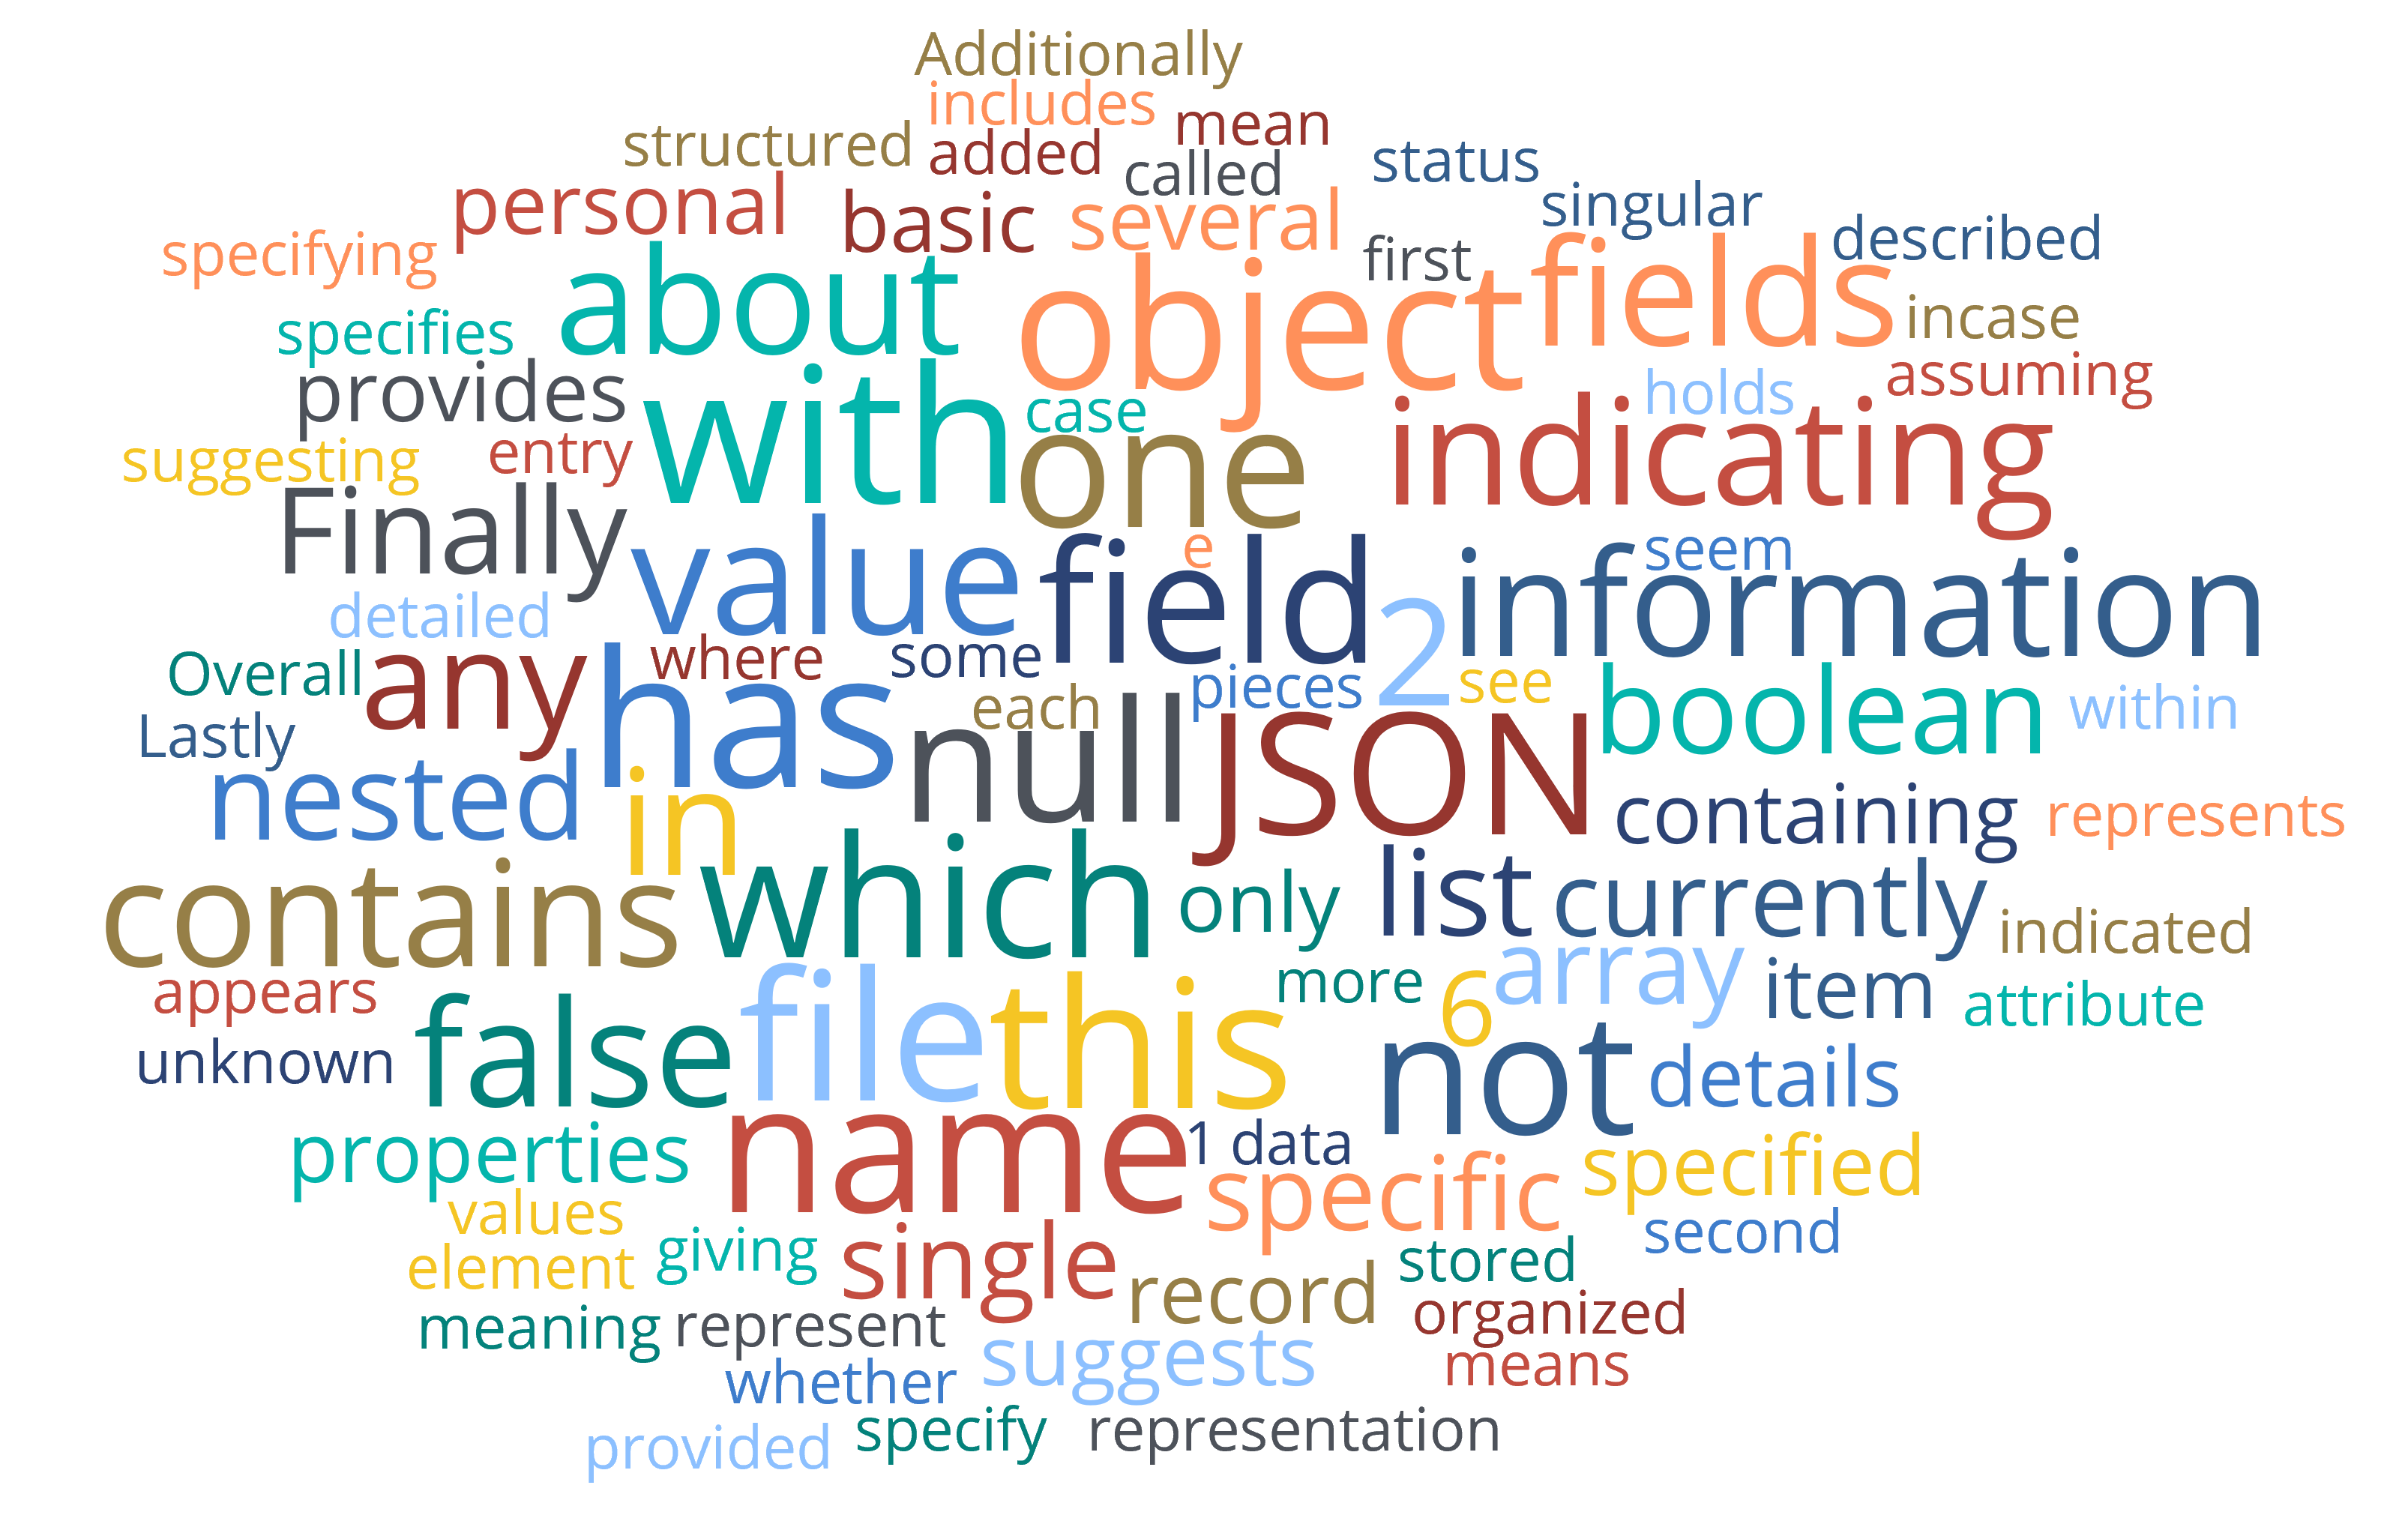
\includegraphics[width=0.4\textwidth]{dissertation/images/Word cloud.png}
    \caption{Word Cloud generated from aggregated descriptions}
    \label{fig:word_cloud}
\end{wrapfigure}

By analysing the language used by programmers to describe JSON files, we were able to develop a formal mapping of the JSON grammar to natural language terms that would be most meaningful and relevant to the intended users of our tool. This research informed our design decisions regarding the levels of detail and customisation options that we built into the tool, ensuring that the tool's descriptions would be both accurate and easily understood by its users. 

Once the data was collected, we aggregated all of the descriptions provided by the students and conducted a word frequency analysis to identify the most frequently used terms to describe the JSON file. To ensure greater clarity, we excluded words that were specific to the given file, such as field names and values, and focused on the commonly used connecting words that are expected to remain constant across different files. From the word frequency analysis, see Table \ref{table:WordFrequency}, we constructed a word cloud, see Figure \ref{fig:word_cloud}, to visualise the words most frequently used by students to describe the JSON file.

\begin{table}[ht]
\small
\caption{Table denoting the frequency of words in the descriptions students gave of Listing \ref{lst:exampleJSON}}
\centering
\begin{tabular}{ |p{1.5cm}|p{1.5cm}||p{1.5cm}|p{1.5cm}||p{1.5cm}|p{1.5cm}| }

\multicolumn{6}{c}{Word Frequency Analysis} \\
\hline
Word& Frequency &Word &Frequency&Word&Frequency\\
\hline
field   & 50&file & 12& information&9\\
has & 40 & not & 12&JSON & 9\\
value & 35 & which & 12& about & 8\\
with & 28& object & 11&in &6\\
of & 18&one & 11&any&5\\
named & 18&this & 10&&\\
indicate & 14&contains&9&&\\

\hline
\end{tabular}
\label{table:WordFrequency}
\end{table}

%\begin{figure}
    %\centering
   % \includegraphics[width=0.5\textwidth]{}
    %\caption{Word Cloud generated from aggregated descriptions}
    %\label{fig:word_cloud}
%\end{figure}




\subsection{Generating a formal description specification}

\begin{wrapfigure}{L}{0.5\textwidth}
    \caption{Initial stages of description design}
    \label{fig:descDesign}
    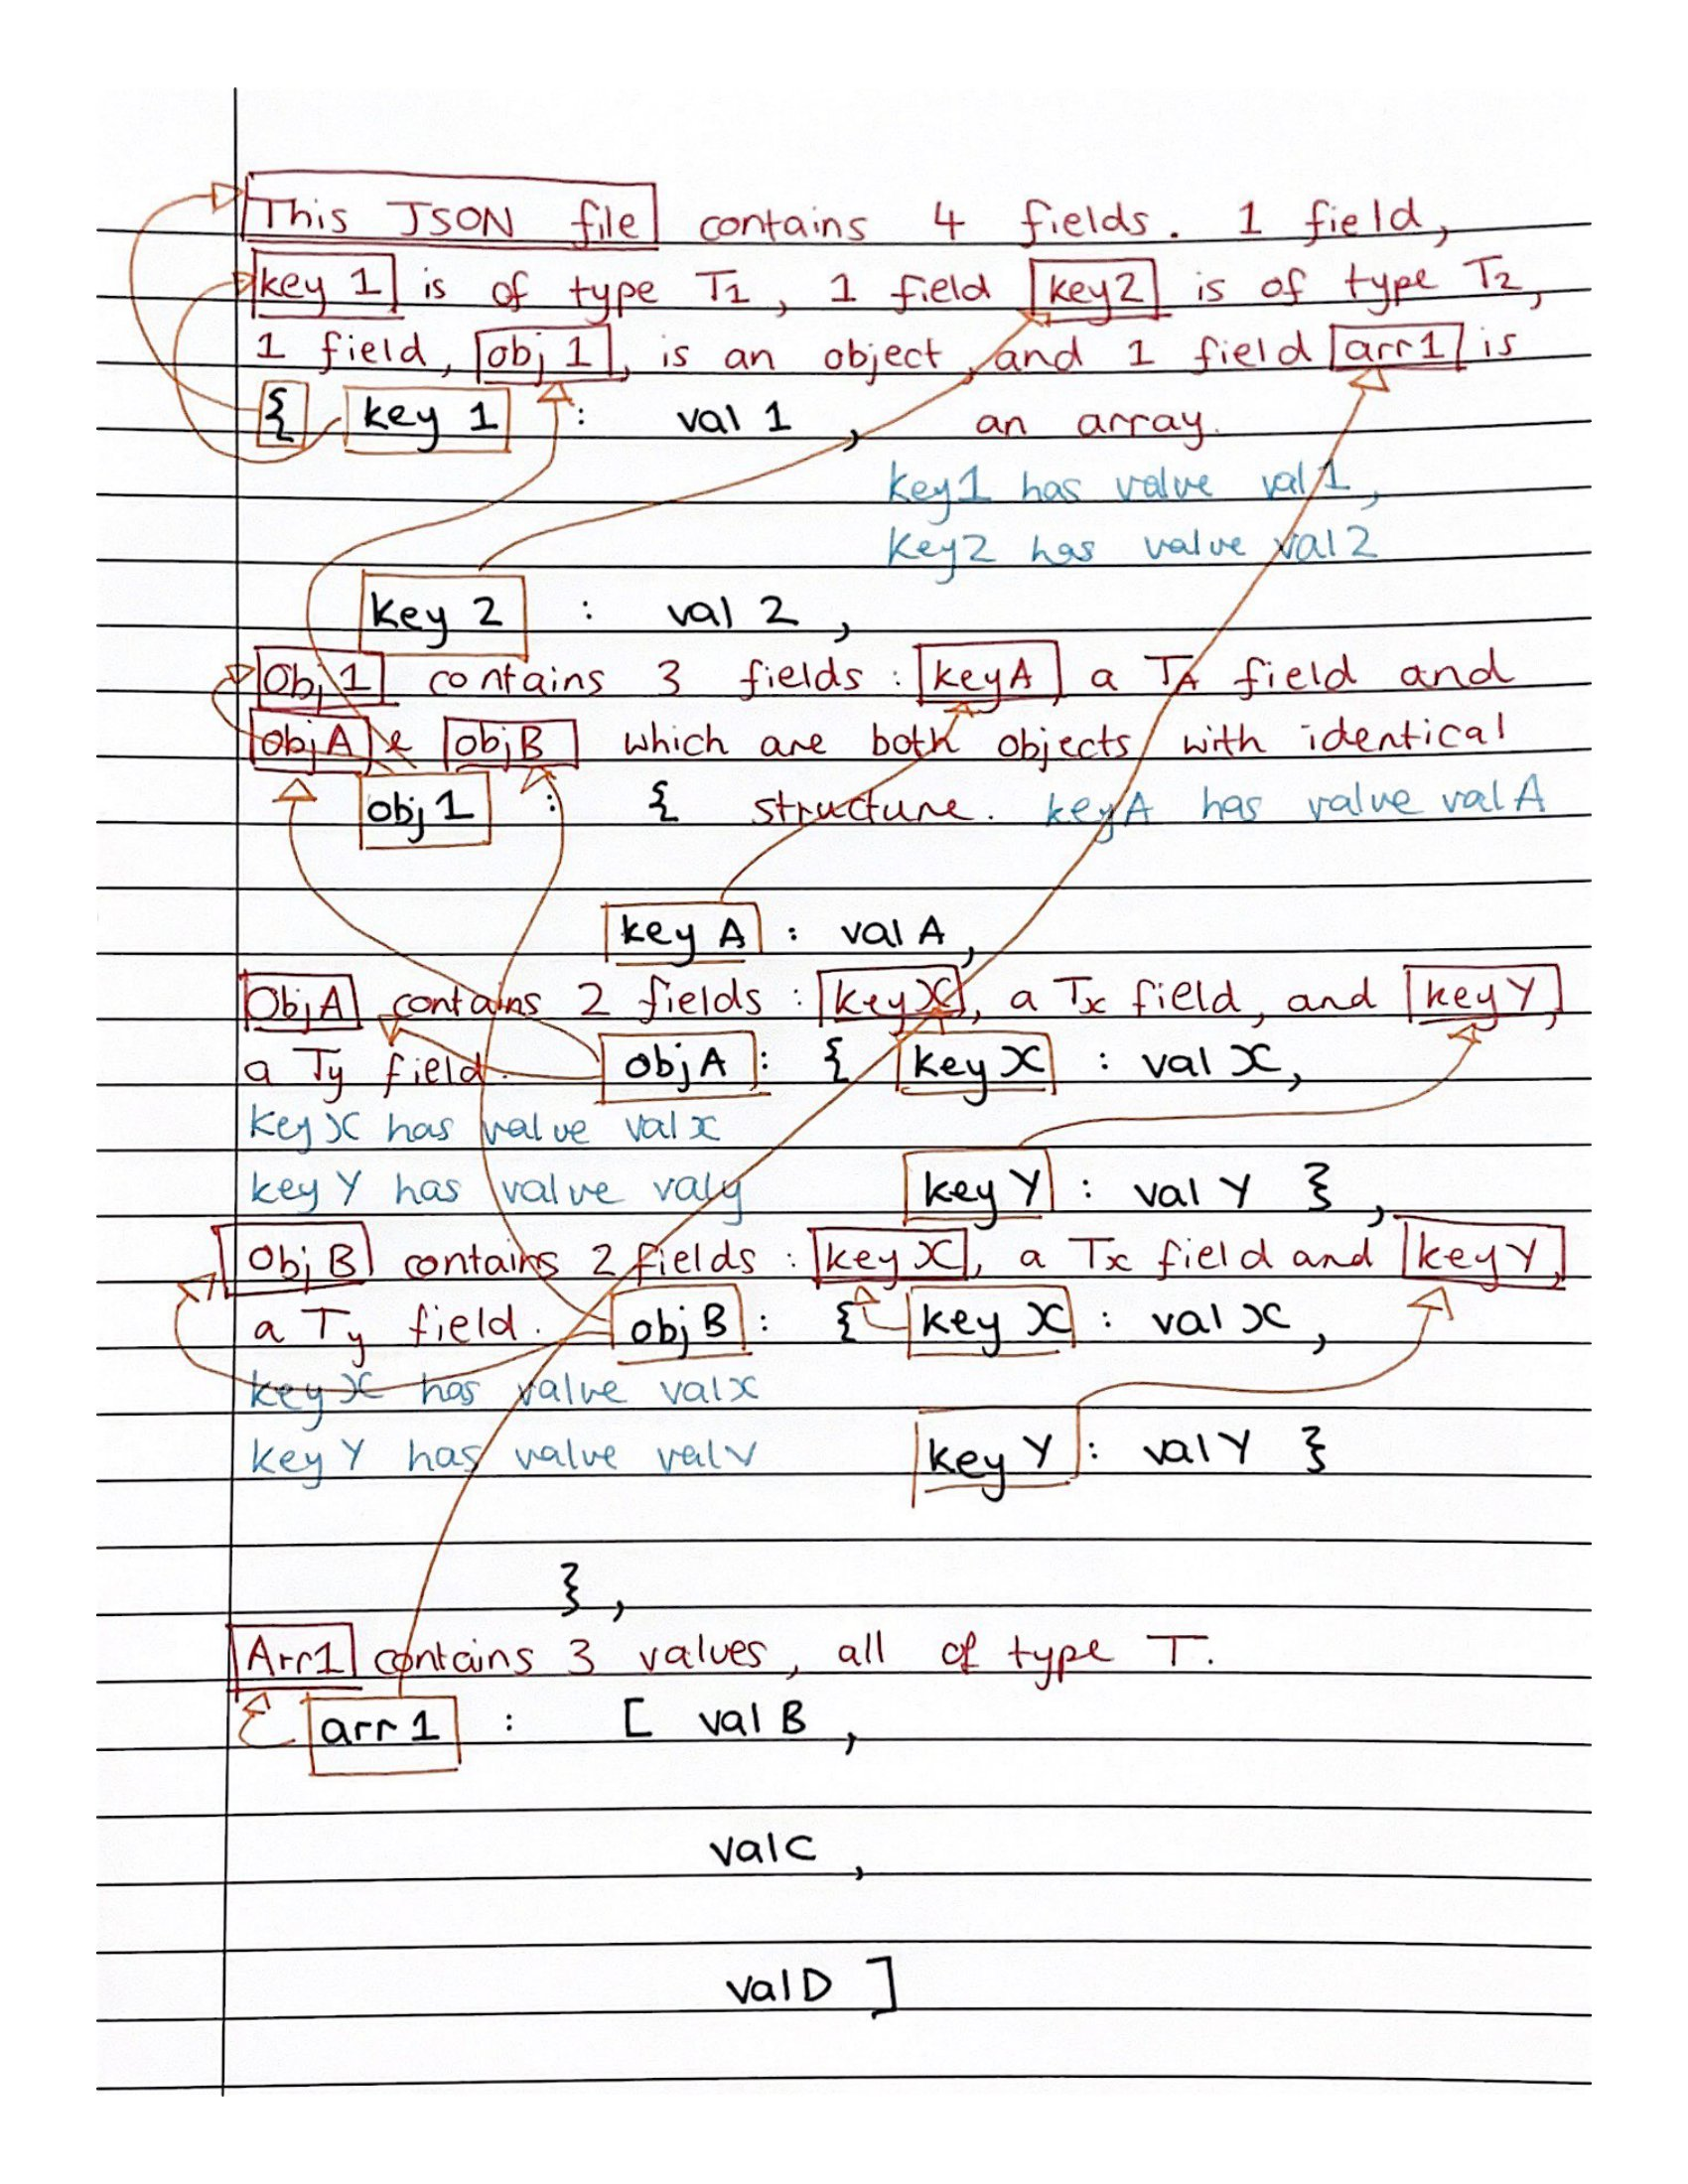
\includegraphics[width=0.5\textwidth]{dissertation/images/Description planning.jpg}
\end{wrapfigure}

Prior to commencing coding, we formulated a formal mapping of the JSON grammar to natural language terminology. Considering the non-customisable nature of utilising a screen reader with a structured text document, we made a design decision to allow the production of varying levels of descriptions with different levels of detail for our tool. Figure \ref{fig:descDesign} illustrates one of the initial steps we took in terms of analysing the JSON file and considering what to include in the description.

\begin{enumerate}
    \item Top-level: This level provides a concise summary of the JSON file, offering users an overall view of the file. It serves as a quick reference point for users who want to understand the file's basic structure without delving into the specifics.
    \item Structural: At this level, we describe the more complex elements of the JSON file, such as objects and arrays, and provide information on the type of elements contained within them. This level helps users understand the relationships and dependencies among different elements in the file.
    \item Full: This level provides a detailed description of each element in the JSON file, including the key and value, or just the value for anonymous elements contained within arrays. It is useful for users who need a complete understanding of the content of the file.
\end{enumerate}
	
In addition to the three levels of description, we also added two more options that users could enable to customise the description further:

\begin{enumerate}
    \item Depth option: This option allows users to specify an integer value that determines the number of levels of elements to describe. This option makes it possible to produce shorter, more understandable descriptions for larger files or files with a high level of nesting. It is an important design goal for our tool to provide users with a better overall view of large files.
    \item Nesting option: If this option is enabled, the depth/nesting level of each compound element is read out to the user, providing context about the information they are hearing. This option helps users better understand the structure of the JSON file and the relationships among its elements.
\end{enumerate}

Shneiderman's work on developing a data type and task taxonomy for information visualisations \cite{Shneiderman_2003} can be applied beyond the visually orientated realm. In fact, the JSONTalk descriptions have been developed in alignment with Shneiderman's mantra for visual information seeking: "overview first, zoom and filter, then details on demand." This approach is reflected in the options provided to users through JSONTalk. Firstly, an overview of the JSON document is provided, allowing users to gain a top-level understanding of the data. Then, users can zoom in on specific information by requesting a full description of the file, which can be filtered by depth or by certain components such as objects and arrays. Finally, users can access the details on demand, requesting that the nesting details of each compound element be displayed. Through these features, JSONTalk provides a comprehensive approach to exploring and understanding JSON data.

\section{Interface design}

We chose to implement the JSONTalk tool as a command-line tool for several reasons. This choice allows us to focus on the core functionality of JSONTalk, without the added complexity of a complicated user interface. A command-line interface serves as a solid foundation for future interface development. Its simplicity makes it an excellent starting point from which to build a more sophisticated user interface, should that become necessary.

Additionally, command-line tools offer greater accessibility for users who require screen readers. This means that users can easily read the description with their own personal screen reader and keep their personal preferences. Additionally, command-line tools offer a more convenient solution for VI programmers than graphical interfaces that rely on visual cues.

Moreover, command-line tools are generally faster and more efficient than graphical interfaces since they do not require the rendering or processing of graphical elements. This efficiency makes command-line tools scalable and adaptable to work with large JSON files.

Furthermore, command-line tools can be easily integrated with other programming tools, improving collaboration among team members and streamlining programming tasks. This integration allows programmers to leverage other tools in their toolkit and work seamlessly between different workflows. 

Overall, implementing the JSONTalk tool as a command-line tool offers a highly accessible, efficient, flexible, and integrated solution for VI programmers working with JSON data. However, it is important to note that even though command-line interfaces are often deemed the most accessible for those with visual impairments, programmers still face a number of accessibility challenges when using the command line. 

\section{Read-aloud functionality}

To ensure accessibility for all users, a read-aloud feature was included in the tool. This feature was intended to provide a more straightforward alternative to using screen reader software with command line interfaces. 
The read-aloud feature was made optional to accommodate users who preferred to use their customised screen reader software.
The goal was to provide a positive and inclusive experience for all users, and flexibility in terms of accessibility features was considered important to achieve this. By providing both the integrated read-aloud feature and the option to use customised screen reader software, we aim to accommodate the diverse needs of users.

The read-aloud feature was implemented using the FreeTTS library. If the read-aloud option is enabled by the user, in addition to being printed on the command line, the description, which is stored as a string, is passed to the TTS engine for speech synthesis. 


 \section{Abstract Syntax Tree analysis}
 \label{section:visitor}
 
In order to plan the syntax of the natural language description and determine the best approach for achieving it, we analysed the ASTs generated by the ANTLR4 tool during the parsing of example JSON files of varying levels of complexity. We were able to do this in the ANTLR Lab \cite{antlrLab}, an interactive tool developed by the creator of ANTLR4, Terence Parr. This allowed us to closely examine the relationships between the various elements and the order in which the nodes would be traversed in the parse tree. This approach helped us gain a deeper understanding of the underlying structure of the JSON files and how best to translate that structure into a clear and concise natural language description.

	

%==================================================================================================================================
\chapter{Implementation}

\section{Resources and technologies used}

We built the JSONTalk tool using Java, with the use of some additional software libraries which are detailed below. The JSONTalk tool is packaged into a jar file which can be run on the command line. We chose Java as it is an object-oriented language, which makes it well-suited for implementing the visitor design pattern, detailed above in section \ref{section:visitor}.

To accelerate the project's development, we leveraged the benefits of various existing libraries. In particular, we utilised the following libraries:

\subsection{Antlr4}

 For crucial initial processing of JSON files, we used Antlr4 (ANother Tool for Language Recognition)\cite{antlr4}. Specifically, for its lexer and parser components, which were instrumental in creating a parse tree from the input JSON files. ANTLR4 played a critical role in implementing the JSONTalk tool by providing a powerful parser generator that allowed us to construct a parse tree from the input JSON file. Using ANTLR4's grammar syntax, lexer, and parser, we were able to extract the syntactic structure of the input and produce an accurate representation of the data.
 
 The subsequent use of a visitor implementation to traverse the parse tree and generate natural language descriptions of the input added significant value to the tool's functionality. ANTLR4's customisable features and reliable performance enabled us to parse the JSON input with precision and efficiency. The use of the Visitor design pattern in combination with ANTLR4 provides a flexible and extensible approach to processing complex data structures.

\subsection{FreeTTS}

For the Read-Aloud functionality of the tool, which enabled users to have the generated natural language descriptions read aloud. FreeTTS \cite{freetts} is a Text-To-Speech (TTS) synthesis system that is used to convert text into speech. It is a Java-based open source software project, which means that it easily integrates with the JSONTalk Java project.  One of the primary reasons to use FreeTTS is that it provides a robust and reliable TTS engine that is freely available to use. This makes it a popular choice for developers who need to add speech output to their projects without having to build their own TTS system from scratch. FreeTTS is designed to be customisable, with the ability to adjust voice characteristics, such as pitch, speed, and volume, to suit different needs.

\subsection{Picocli}

 For implementing the tool as a Command Line Interface (CLI), making it easier for users to access and operate the tool, we used Picocli \cite{picocli}. Picocli is a Java command-line parser library that simplifies the process of creating command-line interfaces for Java applications. Picocli is a lightweight, low-ceremony solution that supports both annotated and programmatic parsing of command-line arguments. It is designed to be easy to use, highly customisable, and to integrate seamlessly with existing Java projects.
    
Using Picocli, we were able to quickly and easily create a user-friendly command-line interface for our JSONTalk tool. Picocli allowed us to define our command-line options and arguments using simple annotations, which made our code more concise and easier to read. Additionally, Picocli provides a wide range of built-in features, such as automatic help and version information.



\section{From JSON to a Natural Language Summary: The Process} 

\begin{wrapfigure}{L}{0.4\textwidth}
    \centering
    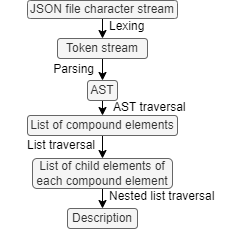
\includegraphics[width=0.4\textwidth]{dissertation/images/jsontodesc.png}    
    \caption{}
    \label{fig:jsontodesc}
\end{wrapfigure}

This section will discuss the classes, functions, and patterns that were required to generate a natural language description. The process is summarised in Figure \ref{fig:jsontodesc}.





%    \begin{center}
%    \fbox{JSON file character stream} \break
 %   \quad \quad $\biggl\downarrow{\text{Lexing}}$ \break
 %   \fbox{Token stream}\break
 %   $\biggl\downarrow{\text{Parsing}}$\break
 %   \fbox{Abstract Syntax Tree}\break
 %   $\biggl\downarrow{\text{AST traversal}}$\break
  %  \fbox{List of compound elements}\break
  %  $\biggl\downarrow{\text{List traversal}}$\break
 %   \fbox{Description}
 %   \end{center}



\subsection{Lexing and parsing a JSON file} 

Using a grammar, ANTLR4 can automatically generate code for a lexer and parser that can be used to recognise and parse input written in the defined language. To avoid the time-consuming task of writing a JSON grammar from scratch, we obtained a pre-existing ANTLR4 grammar file from "The Definitive ANTLR4 Reference", written by Terence Parr, the creator of ANTLR4\cite{parr2013definitive} (see Appendix \ref{appendix:grammar} for the grammar). In addition, ANTLR generates tree walkers automatically, which can be used to traverse the nodes of such trees and execute customised code specific to the application. Following the execution of the ANTLR4 tool with the JSON grammar, the corresponding lexing and parsing classes, as well as a visitor interface, were generated. Based on this interface, we developed the jsonDescriptorVisitor class.

%he visitor design pattern was employed to traverse each node of the AST generated from parsing the input JSON files. By doing so, we were able to extract the necessary information required for the description from each node, which was then stored in various objects.

%The jsonElement object was utilised to store information regarding primitive JSON key-value pairs, including both named and anonymous pairs. Such values were defined as being of type STRING, NUMBER, BOOLEAN, or NULL. To store information about complex JSON key-value pairs, the jsonComplexElement class was created as an extension of the jsonElement class. The jsonComplexElement class was used to store values that were of type OBJECT and ARRAY.

%Furthermore, the jsonObject class extended the jsonComplexElement class and provided additional functionality that catered specifically to JSON objects. Similarly, the jsonArray class was also created as an extension of the jsonComplexElement class and provided functionality tailored to JSON arrays. Figure \ref{fig:JSON element class diagram} illustrates the relationships between these classes.




%In order to provide users with precise nesting and depth information for each JSON element, we implemented a system in which nodes were added to a list of their parent node's "children" while traversing the AST. This ensured that each parent node was always a jsonComplexElement.

%By utilising this approach and storing each element as a child of its respective parent, we were able to generate a comprehensive file description. Specifically, we iterated through each jsonComplexElement object that was created and listed the details of its children. This double traversal technique of traversing the parse tree, creating objects, adding them to a new data structure and traversing it allowed for greater freedom in the generation of the description. Extracting the logic for the description generation from the visitor allowed for more readable code, and gave classes single responsibility. This allowed us to accurately represent the hierarchical structure of the JSON file and provide the user with detailed information on the contents of each element.

\subsection{Visitor Design Pattern}

We used the visitor design pattern \cite{hunt2013gang} to traverse every node in the Abstract Syntax Tree (AST) that resulted from parsing the input JSON files. The visitor design pattern is a behavioural design pattern that allows us to separate an algorithm from an object structure on which it operates. This enabled us to extract the necessary information from each node, which we stored in various objects: namely jsonElement, jsonComplexElement, jsonObject, and jsonArray objects.

For primitive JSON key-value pairs (both named and anonymous), we utilised the jsonElement object to store the relevant information. These values were classified as STRING, NUMBER, BOOLEAN, or NULL. On the other hand, we created the jsonComplexElement class as an extension of jsonElement to store information about complex JSON key-value pairs of type OBJECT and ARRAY.

To provide additional functionality specific to JSON objects and arrays, we further extended the jsonComplexElement class to create the jsonObject and jsonArray classes, respectively. The relationships between these classes are illustrated in Figure \ref{fig:JSON element class diagram}.

To provide users with accurate nesting and depth information for each JSON element, we implemented a system in which nodes were added to a "children" list of their respective parent node while traversing the AST. By listing each element as a child of its parent, we were able to represent the hierarchical structure of the JSON file accurately. Moreover, this approach simplified the description generation logic and allowed us to iterate over each jsonComplexElement object and list its children's details efficiently.

By extracting the logic for the description generation from the visitor, we not only made the code more readable but also adhered to the SOLID single responsibility principle \cite{martin2000design} Each class was given a single responsibility, making it easier to understand and maintain the code-base. The jsonObject and jsonArray classes, for instance, were responsible for providing additional functionality tailored to their respective JSON element types. This approach not only increased the code's modularity but also made it easier to extend and modify the functionality in the future.

\subsection{Class breakdown}

\subsubsection{Classes for initial JSON processing}\hfill

\paragraph{\textbf{jsonLexer}:} Takes the character stream from the input JSON file and generates a series of tokens, which are passed to jsonParser to create the abstract syntax tree.

\paragraph{\textbf{jsonParser}:} Takes the token stream generated by jsonLexer and turns it into an abstract syntax tree.

\paragraph{\textbf{jsonDescriptorVisitor}:} Implements jsonVisitor and uses the visitor design pattern to generate jsonElement, jsonObject, or jsonArray objects from nodes in the parse tree. These objects are stored in a data structure.


\begin{figure}[h]
    \centering
    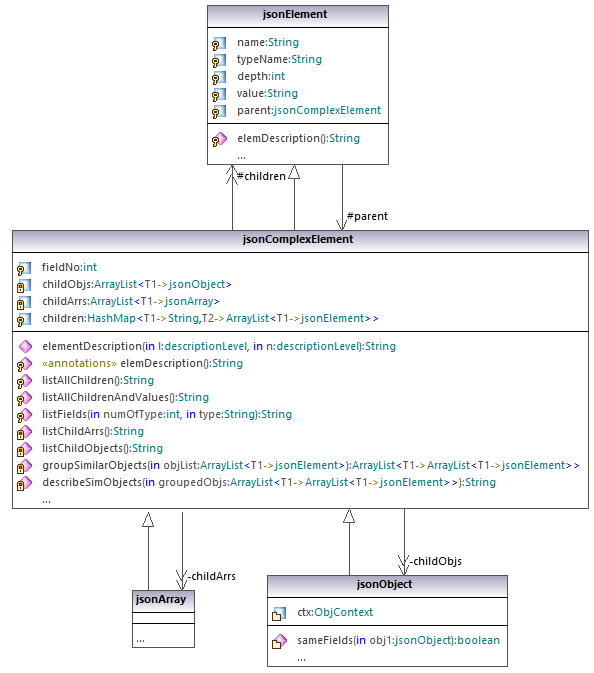
\includegraphics[width=0.7\textwidth]{dissertation/images/JSONElements class diagram.png}
    \caption{Class diagram for the JSON element, complex element, object, and array classes}
    \label{fig:JSON element class diagram}
\end{figure}

\subsubsection{Classes to generate element specific descriptions} \hfill 

\paragraph{\textbf{jsonElement}:} Holds information about primitive jsonElements, such as string, integer, Boolean, and null values. The information includes the name of the element (if any), type, depth, value, and parent. This class generates a simple description of the element based on its stored values, which can be used in larger description generation methods.

\paragraph{\textbf{jsonComplexElement}:} Extends jsonElement and is the parent class of jsonObject and jsonArray. This shared parent allows the data structure generated by jsonDescriptorVisitor to hold both arrays and objects as keys in the same hashmap. In addition to the fields in jsonElement, jsonComplexElement has four more fields: FieldNo, which represents the number of child elements within the complex element; children, which is a hashmap of the child elements categorized by type; and separate lists of the objects and arrays that are children of the complex element. These additional fields simplify description generation when the "objectsandarrays" option is enabled.

jsonComplexElement has larger description generation methods which when called will return a string describing the element and all child elements of the complexElement. The options specified by the user on the command line determine what description generation methods to be called.

\paragraph{\textbf{jsonObject}:} A subclass of jsonComplexElement that holds information specifically about objects. When an object node is visited by jsonDescriptorVisitor's visitObject method, a jsonObject object is instantiated. jsonObject includes an additional objectContext field, which is used in methods that compare jsonObjects to determine if they have the same structure (i.e., the same fields but different values).

\paragraph{\textbf{jsonArray}:} A subclass of jsonComplexElement that holds information specifically about arrays. When an array node is visited by jsonDescriptorVisitor's visitArray method, a jsonArray object is instantiated.\hfill \break

\subsubsection{Class for whole descriptions generation} \hfill

\paragraph{\textbf{jsonRun}:} Traverses the data structure created by JSONDescriptorVisitor as it visits the nodes on the parse tree generated by JSONParse. As jsonRun traverses the data structure created by jsonDescriptorVisitor, the description string is built up by calling the jsonComplexElement elementDescription method, passing the command-line options which have been converted to an enum representation for simplicity.\hfill
\break

\subsubsection{Classes for user interface} \hfill 

\paragraph{\textbf{jsonCLI}:} This class handles the command line interface: it processes user input and produces user output. The command-line arguments and options are parsed, and the JSON file is turned into an AST using jsonLexer lex() and jsonParser parse() methods. The AST is passed to the jsonRun describe() method, along with a Boolean representation of the command-line options selected by the users. The describe() method returns a String containing the requested JSON description, and if requested, jsonCLI will write the description to a file or pass it to the TextToSpeech SpeakString() method for reading out.

\paragraph{\textbf{TextToSpeech}:} This class is responsible for the TTS functionality behind the read-aloud feature of the JSONTalk tool. It uses a Synthesis Engine imported from FreeTTS \cite{freetts}. It has a SpeakString method which takes a string input and synthesises a speech representation of the string. The SpeakString method is called by the jsonCLI class if the user enables the read-aloud command line option.



%==================================================================================================================================
\chapter{Evaluation of JSONTalk: User study} 

\section{Methodology}



\subsection{Evaluation questions}
Research questions for evaluation to answer:
\begin{enumerate}
\item Does JSONTalk accurately represent the contents of a JSON file?
\item Does JSONTalk allow users to quicker understand the structure and contents of a JSON file compared to when it is represented by a screen reader?
\item Does JSONTalk help users identify the context of individual key-value pairs within the JSON file?
\item Does JSONTalk help users identify the presence of objects with identical structure?
\item Is the JSONTalk tool usable?
\end{enumerate}

\subsection{Recruitment of sighted programmers}
The evaluation was carried out with the participation of sighted programmers, rather than VI programmers. Prior to the evaluation, we conducted a feasibility study to determine the viability of engaging VI programmers in the evaluation. Based on the project timeline, we arrived at the conclusion that an evaluation with sighted programmers would be more appropriate.

As the primary target users of the JSONTalk tool comprise VI programmers who use screen readers and other assistive technologies to perform programming tasks, the sighted users were presented with screen reader transcripts of the JSON files instead of the JSON files themselves. This approach ensured that the use case of the tool was represented more realistically.

\subsection{Evaluation overview}
The evaluation was carried out in the form of a between-subjects A/B test, where participants were required to answer a series of questions related to three different JSON file screen reader transcripts. The A group answered the questions using the JSONTalk tool, while the B group answered the questions without the tool. The evaluation was carried out online through a survey consisting of the following sections.

To ensure that all participants were on a level playing field when it came to prior familiarity with JSON, both groups were primed on JSON syntax. Although all participants who were recruited had a strong programming background, this primer was included to ensure that the potential differences in JSON knowledge did not confound the results.

Next, the A group was shown how to download and use the JSONTalk tool, after which both groups were presented with three JSON file screen reader transcripts and asked to answer three specific questions. The A group was allowed to use the JSONTalk tool to help them decipher the contents of the JSON file from the screen reader transcript, while the B group was not provided with any additional tools. The tasks that participants were required to complete were as follows:

\begin{enumerate}
    \item Determine the level of nesting of a particular object
    \item Determine whether there are any objects with duplicate structures (i.e. same keys) within the JSON file
    \item Rewrite the JSON file into its original syntax
\end{enumerate}

We chose question (1), due to the context issues faced by VI programmers when reading a JSON file with assistive technology. Determining the level of nesting of a particular object is essentially determining the context of a specific object. The results of this question will help us answer research question (3).

We selected question (2) because in JSON files, the presence of multiple identical object structures often suggests that these objects represent a collection or a related set of data. By identifying which object structures are identical, users can gain a deeper understanding of the information conveyed by the JSON file. Although JSONTalk does not provide explicit guidance on how to use the data, clarifying the identical object structures within a JSON file can aid users in comprehending the file's broader purpose and potential applications. The results of this question will help us answer research question (4)

We selected question (3), to determine whether the JSONTalk tool accurately represents JSON files. Observing what users think is the underlying JSON file and comparing the answer to the actual file used to generate the description is a good way to measure the accuracy of the JSONTalk tool. The results from this question will inform our answer to research question (1).

We chose to record the time it took for users to answer the above questions to help us answer research question (2).

Following the completion of the tasks, the A group was asked to fill out a System Usability Scale matrix based on their experience with the JSONTalk tool. The results from this will help us answer research question (5).

The decision to use a design of A / B testing between subjects for this evaluation was made to enable a direct comparison between the A and B groups, while reducing the potential impact of individual differences in participant characteristics. By priming all participants on JSON syntax, the potential differences in prior JSON knowledge between the groups were minimised. Additionally, by limiting the use of the JSONTalk tool to the A group, we were able to assess the effectiveness of the tool in facilitating the completion of the tasks while also providing a fair comparison of the performance between the two groups. The use of an online survey format for the evaluation allowed for efficient data collection from a geographically diverse set of participants.

\cite{JSON}

\subsection{Data collected}

The evaluation collected various types of data to assess the effectiveness of the JSONTalk tool. The error rate for each question was collected, allowing for an assessment of the accuracy of the responses provided by the participants. Furthermore, the similarity between the JSON files rewritten by the participants and the actual JSON file used was measured. This provided insight into the ability of participants to accurately understand and replicate the syntax of the JSON file.

The time it took users to complete each task was also recorded, providing an indication of the relative efficiency of using the JSONTalk tool to complete the tasks. Finally, the answers to the System Usability Survey were collected, which allowed participants to provide their feedback on their experience using the JSONTalk tool. This data was then used to determine the level of user satisfaction with the tool, as well as any areas for improvement.


\section{Results}


\subsection{Participant overview}

The study was carried out remotely and the participants completed it online; the full survey can be viewed in the Appendix \ref{appendix:study}. We received a total of 40 responses. Participants in Group A were required to download JSONTalk, which was packaged as a jar file, as well as three JSON files used in the study. JSONTalk needed to be run on the command line. To ensure that participants in Group A could effectively use the tool, a comprehensive introduction to the tool was provided at the start of the study, along with instructions on how to run it.

Given the command-line usage requirements of the tool, participants with a programming background who were familiar with such tools were recruited. Most participants were sourced from the University of Glasgow Computer Science department, including computer science students and university staff. However, a small number of external participants, including professional software developers and computer science students from other universities, also participated in the study. While demographic information can be useful in analysing study results, it was not deemed necessary for the purposes of this study. We also wanted to keep the study as short and focused as possible to encourage higher completion rates \cite{deutskens2004response}.

This section presents the findings of our study. To test for significant differences between the two groups, we used the null hypothesis testing framework. Our chosen threshold for determining statistical significance was a p-value of 0.05.



Participants in group A were provided with instructions on how to use the JSONTalk tool on the command line for the underlying JSON file of each question. Although we encouraged participants to use the tool to supplement the screen reader transcript, we explicitly asked after each question whether they had used the tool, to minimise the risk of obtaining misleading results. If a participant in group A reported not using the tool to answer a question, their response for that question was excluded from group A's results and added to group B's results. This method resulted in uneven group sizes for each question. However, to accurately measure the effect of the JSONTalk tool, we considered this trade-off necessary.

\subsection{Statistical methods}

In our study, we wanted to investigate whether there was a significant difference in the timing of responses between both groups of participants. Analysis of the collected data revealed that the time it took participants to answer each question was not normally distributed. As a result, we opted to use the Mann-Whitney U test statistic to test the hypothesis.
The Mann-Whitney U test is a non-parametric test that allows us to compare two independent samples and determine if they come from the same population or not. In our case, we used this test to compare the time taken by participants to answer each question in two different conditions.

 We also wanted to investigate whether there was a significant difference in the accuracy of responses between different groups of participants.
We organised our data into a contingency table, where the rows represent the different experimental conditions, and the columns represent the accuracy of responses or type of mistake (dependant on the question). We then calculated the expected frequencies of each cell in the contingency table under the assumption that there was no association between the experimental conditions and the accuracy of responses.

\subsection{Question breakdown}

\subsubsection{Question 1: Answering a depth and structure question based on a written screen reader transcript} \hfill


%%\begin{minipage}{0.49\textwidth}
\begin{wrapfigure}{R}{0.45\textwidth}
    \centering
    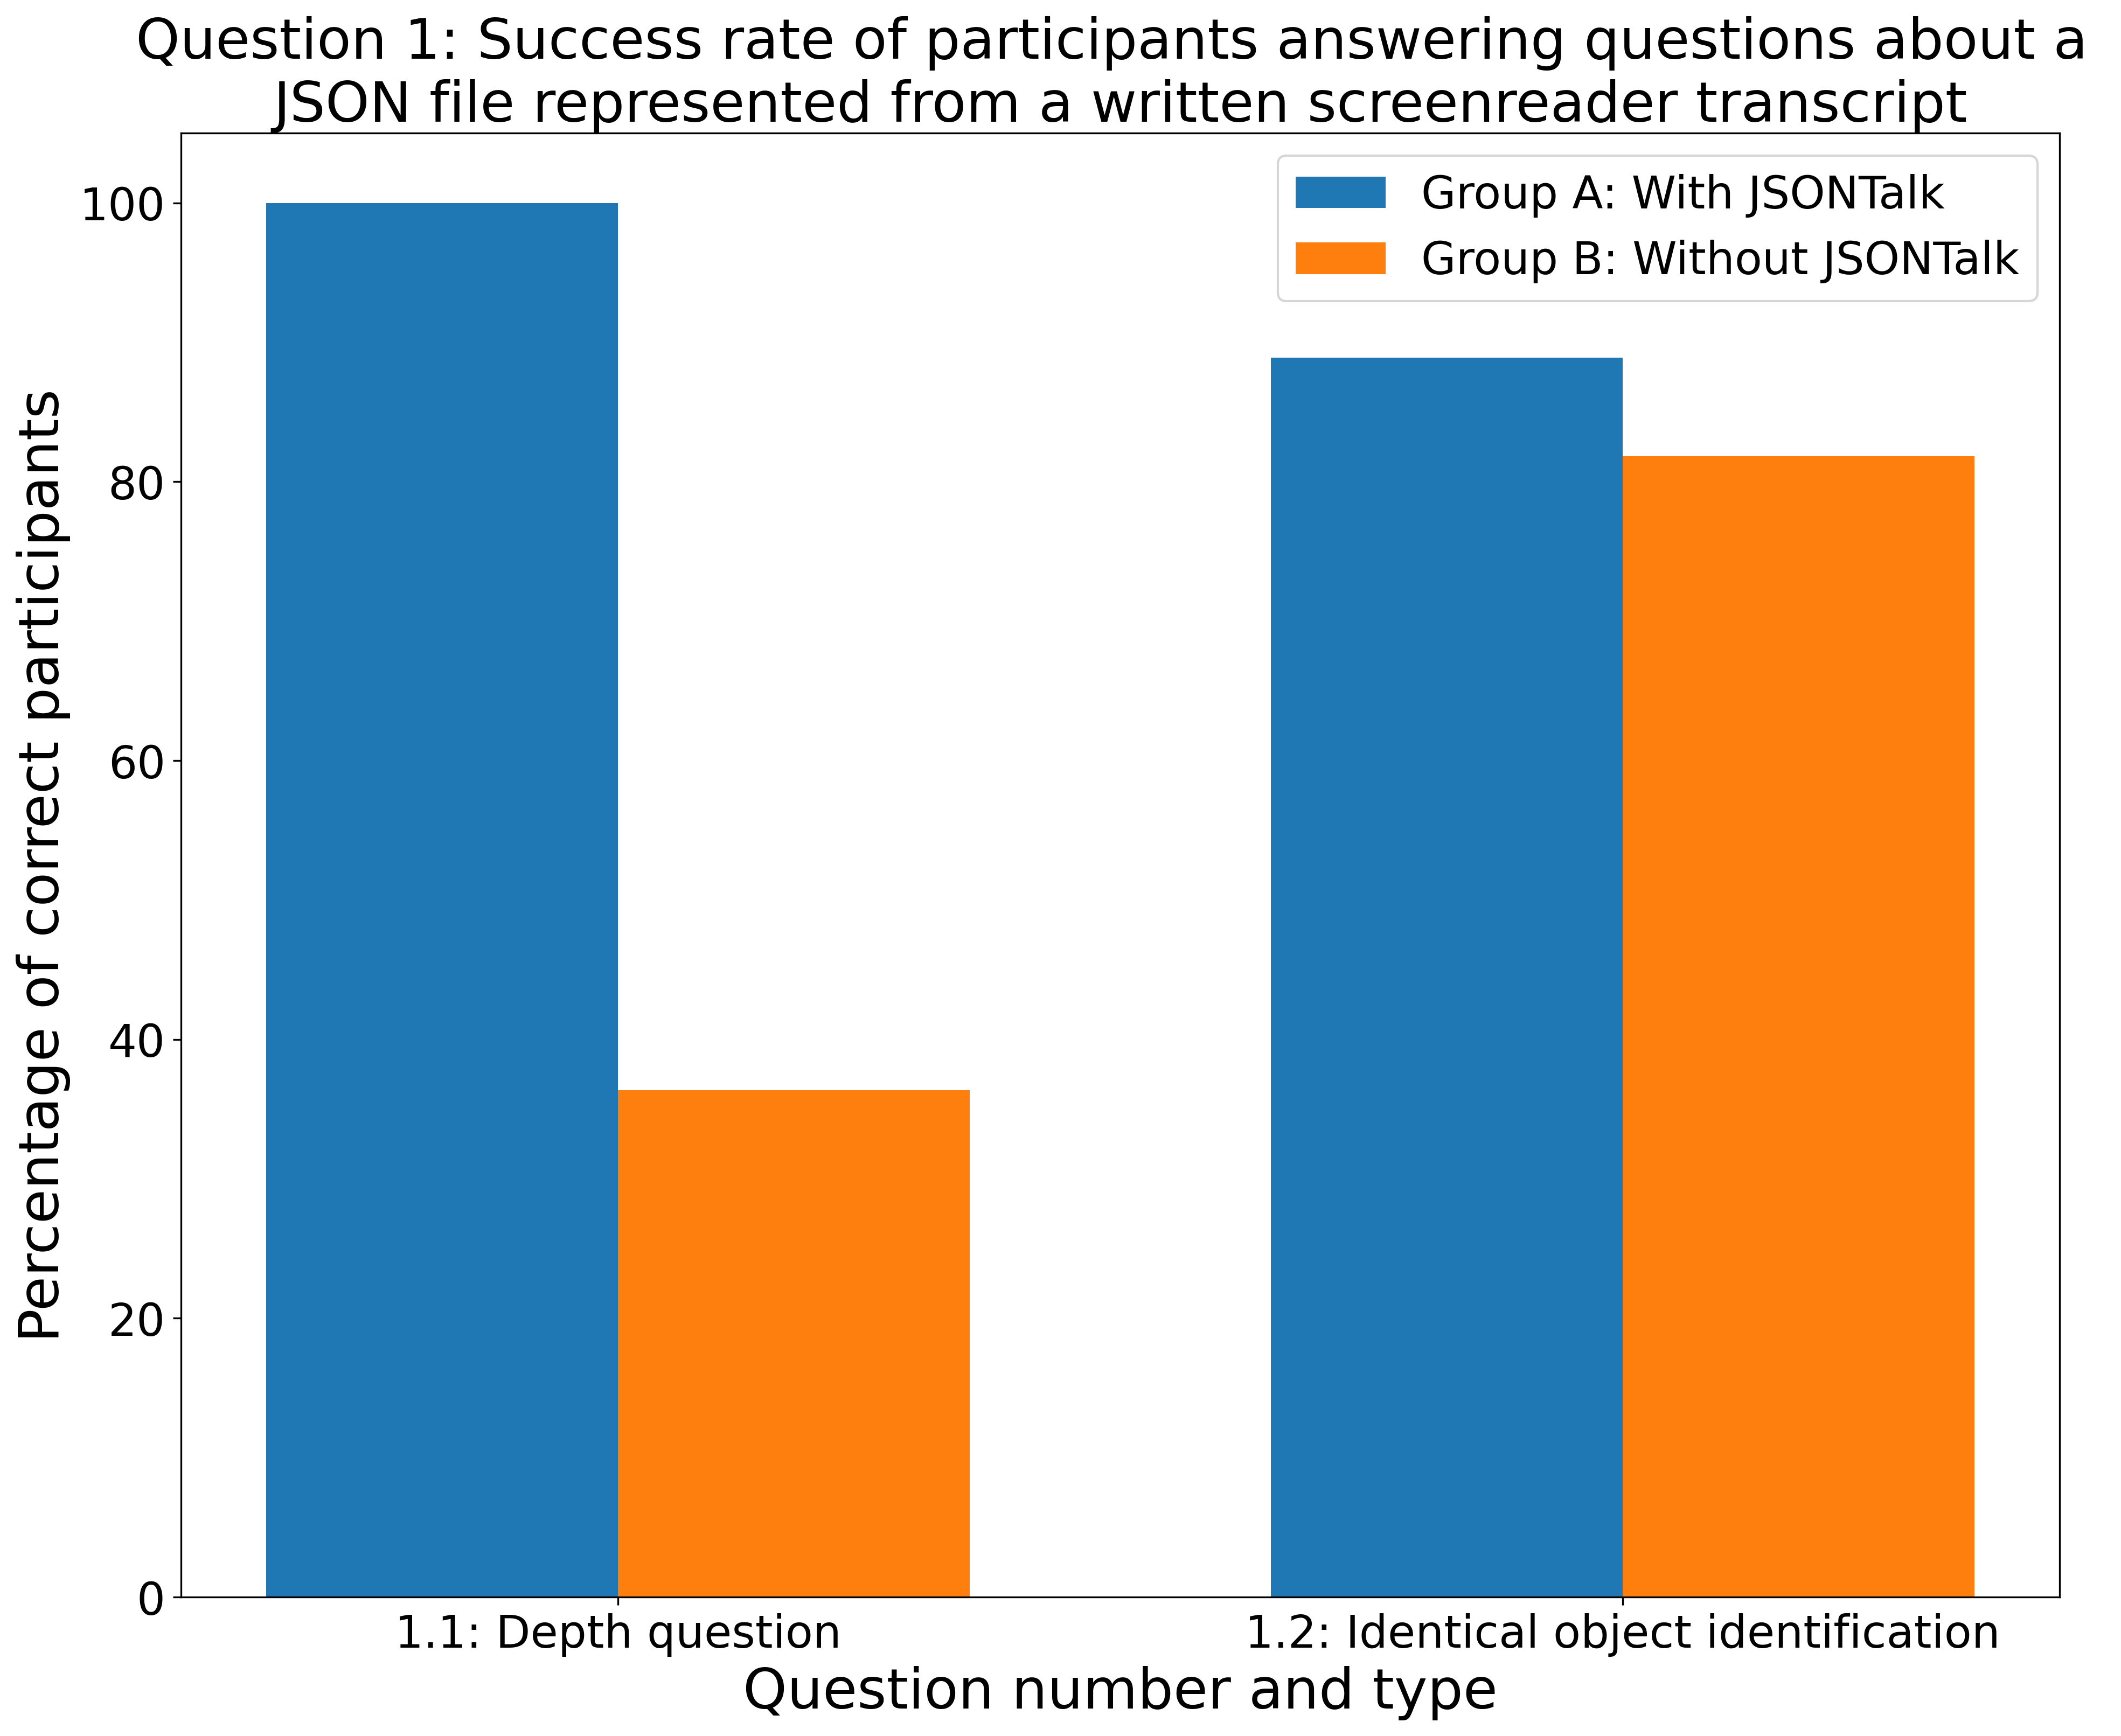
\includegraphics[width=0.45\textwidth]{dissertation/images/Evaluation results/Question 1_ Success rate of participants answering questions about a _JSON file represented from a written screenreader transcript.png}
    \caption{}
    \label{fig:q1graph}
\end{wrapfigure}
%%\end{minipage}
%
%%\begin{minipage}{0.49\textwidth}
\begin{table}[ht]
\small
\centering
\centerline{
\begin{tabular}{p{0.22\textwidth}|p{0.8\textwidth}}
\multicolumn{2}{c}{\textbf{Question 1.1 statistical analysis}} \\ \hline
{Null hypothesis} & There is no significant difference between the number of participants to answer a depth based question correctly using or not using the JSONTalk tool \\ \hline
{Chi-square statistic} & 14.9362 \\ \hline
{P-value} & 0.0001 \\ \hline
{Degrees of freedom} & 1 \\ \hline
{Conclusion} & \textbf{Null hypothesis rejected} \\ 
\end{tabular}
}
\end{table}
%%\end{minipage}



Question 1 of the study involved participants viewing a written transcript of what a screen reader would read if it were to encounter a relatively simple JSON file, named "a.json". The file contained nested objects and arrays, and we intentionally kept it short and simple enough to challenge participants without overwhelming them. All participants were given the same screen reader transcript of the JSON file and were asked to answer two questions designed to assess their comprehension of the file's structure.

\paragraph{Question 1.1: Depth based question} \hfill

The first part asked participants to determine the depth of object "y" if object "x" was located at depth 1. The data was then processed by encoding each answer as correct or incorrect. We found that 100\% of participants in group A answered correctly, whilst 36.36\% of participants in group B answered correctly.

A Chi-square test was conducted on the results to determine whether there is a significant difference in participants' ability to answer a depth question correctly with or without the use of the JSONTalk tool. The test yielded a p-value lower than 0.05, indicating that the difference observed is statistically significant. Therefore, we can conclude that there is a significant difference between the two groups in their ability to answer the depth question.






\paragraph{Question 1.2: Identical object identification}\hfill

The second part required participants to identify whether any objects in the underlying JSON file had identical structures. To clarify the second question, the participants were given an explanation of what it means for objects to have identical structures. For this, participants were required to choose one of 3 options (yes, no, unsure), and during processing, the data was encoded as correct, incorrect, or unsure. We found that 88.89\% of participants from group A answered this correctly, 5.56\% were unsure, and 5.56\% were incorrect. 
In group B, 81.82\% of the participants were correct, 9.09\% were unsure and 9.09\% were incorrect. 

A Chi-square test was conducted on the results to determine whether there is a significant difference in participants' ability to answer an object structure question correctly with or without the use of the JSONTalk tool. The test yielded a p-value higher than 0.05, indicating that the difference observed is not statistically significant. Therefore, we can conclude that the tool does not have a significant effect on participants' ability to identify the presence of identical objects.


\begin{table}[ht]
\small
\centering
\centerline{
\begin{tabular}{p{0.22\textwidth}|p{0.8\textwidth}}
\multicolumn{2}{c}{\textbf{Question 1.2 statistical analysis}} \\ \hline
{Null hypothesis} & There is no significant difference between the number of participants to correctly identify identical objects within a JSON file using or not using the JSONTalk tool \\ \hline
{Chi-square statistic} & 0.8000 \\ \hline
{P-value} & 0.6703 \\ \hline
{Degrees of freedom} & 2 \\ \hline
{Conclusion} & \textbf{Null hypothesis accepted} \\ 
\end{tabular}
}
\end{table}



\paragraph{Additional observations}\hfill
In particular, the two groups show contrasting patterns of success in both parts of question 1. Specifically, while Group A excelled in the depth-based question compared to the identification of identical objects, Group B demonstrated better performance in the latter than in the former.

\paragraph{Question 1 Timing}\hfill

We recorded the time it took the participants to complete Question 1, both with and without the tool. Group A took an average of 265.44 s to complete question 1, and group B took an average of 316.06 s to complete the question. 

To determine whether there is a statistically significant difference between the completion times, we performed a Mann-Whitney U test on the results. The test produced a p-value higher than 0.05, indicating that the observed difference is not statistically significant. Therefore, we conclude that the tool does not have a significant effect on the completion time of question 1, compared to completing the question without the tool.


\begin{table}[ht]
\small
\centering
\centerline{
\begin{tabular}{p{0.22\textwidth}|p{0.8\textwidth}}
\multicolumn{2}{c}{\textbf{Question 1 overall timing statistical analysis}} \\ \hline
{Null hypothesis} & There is no significant difference between the time it takes participants to answer 2 questions about a JSON file using or not using the JSONTalk tool \\ \hline
{Mann-Whitney U test} & 137.0000 \\ \hline
{P-value} & 0.1000 \\ \hline
{Effect size (Cohen's d)} & -0.5270 \\ \hline
{Conclusion} & \textbf{Null hypothesis accepted} \\ 
\end{tabular}
}
\end{table} 


\subsubsection{Question 2: Rewriting a JSON file from a written screen reader transcript}\hfill

In Question 2, participants were presented with a written screen reader transcript of a small (23 lines) JSON file. Participants were asked to rewrite the screen reader transcript into the original JSON file that it was representing. All participants were presented with the same written transcript, and again group A were reminded of how to run the JSONTalk to generate descriptions of the corresponding JSON file. We processed the data as follows:

\begin{itemize}
\item Any necessary punctuation was added or removed to make the JSON file valid
\item Answers were fed into a semantic JSON comparison tool \cite{grossbart}, being compared to the original JSON file which the transcript was based on.
\item The comparison yielded results pertaining to the number of differences of different categories. These results were recorded for each answer.
\end{itemize}

We made minor syntactic adjustments to ensure that the JSON syntax is valid for two reasons. First, the semantic comparison tool only accepts JSON files with valid syntax. Second, our main focus in this question is to investigate whether the JSONTalk tool helps users comprehend the meaning of a JSON file more effectively than a screen reader reading the raw file. Therefore, we aim to concentrate on semantic discrepancies rather than insignificant syntactic differences that can be easily rectified.

In terms of error categories, 3 different categories of errors were observed:
\begin{itemize}
    \item Missing properties: A property present in the original JSON file was not present in the rewritten JSON file.
    \item Unequal values: A value in the rewritten JSON file was not the same as the value in the original JSON file for.
    \item Incorrect type: A value in the rewritten JSON file was of a different type to the same value in the original JSON file. 
\end{itemize}

\paragraph{Total number of mistakes}\hfill
\begin{figure}
    \centering
    \begin{subfigure}{0.49\textwidth}
        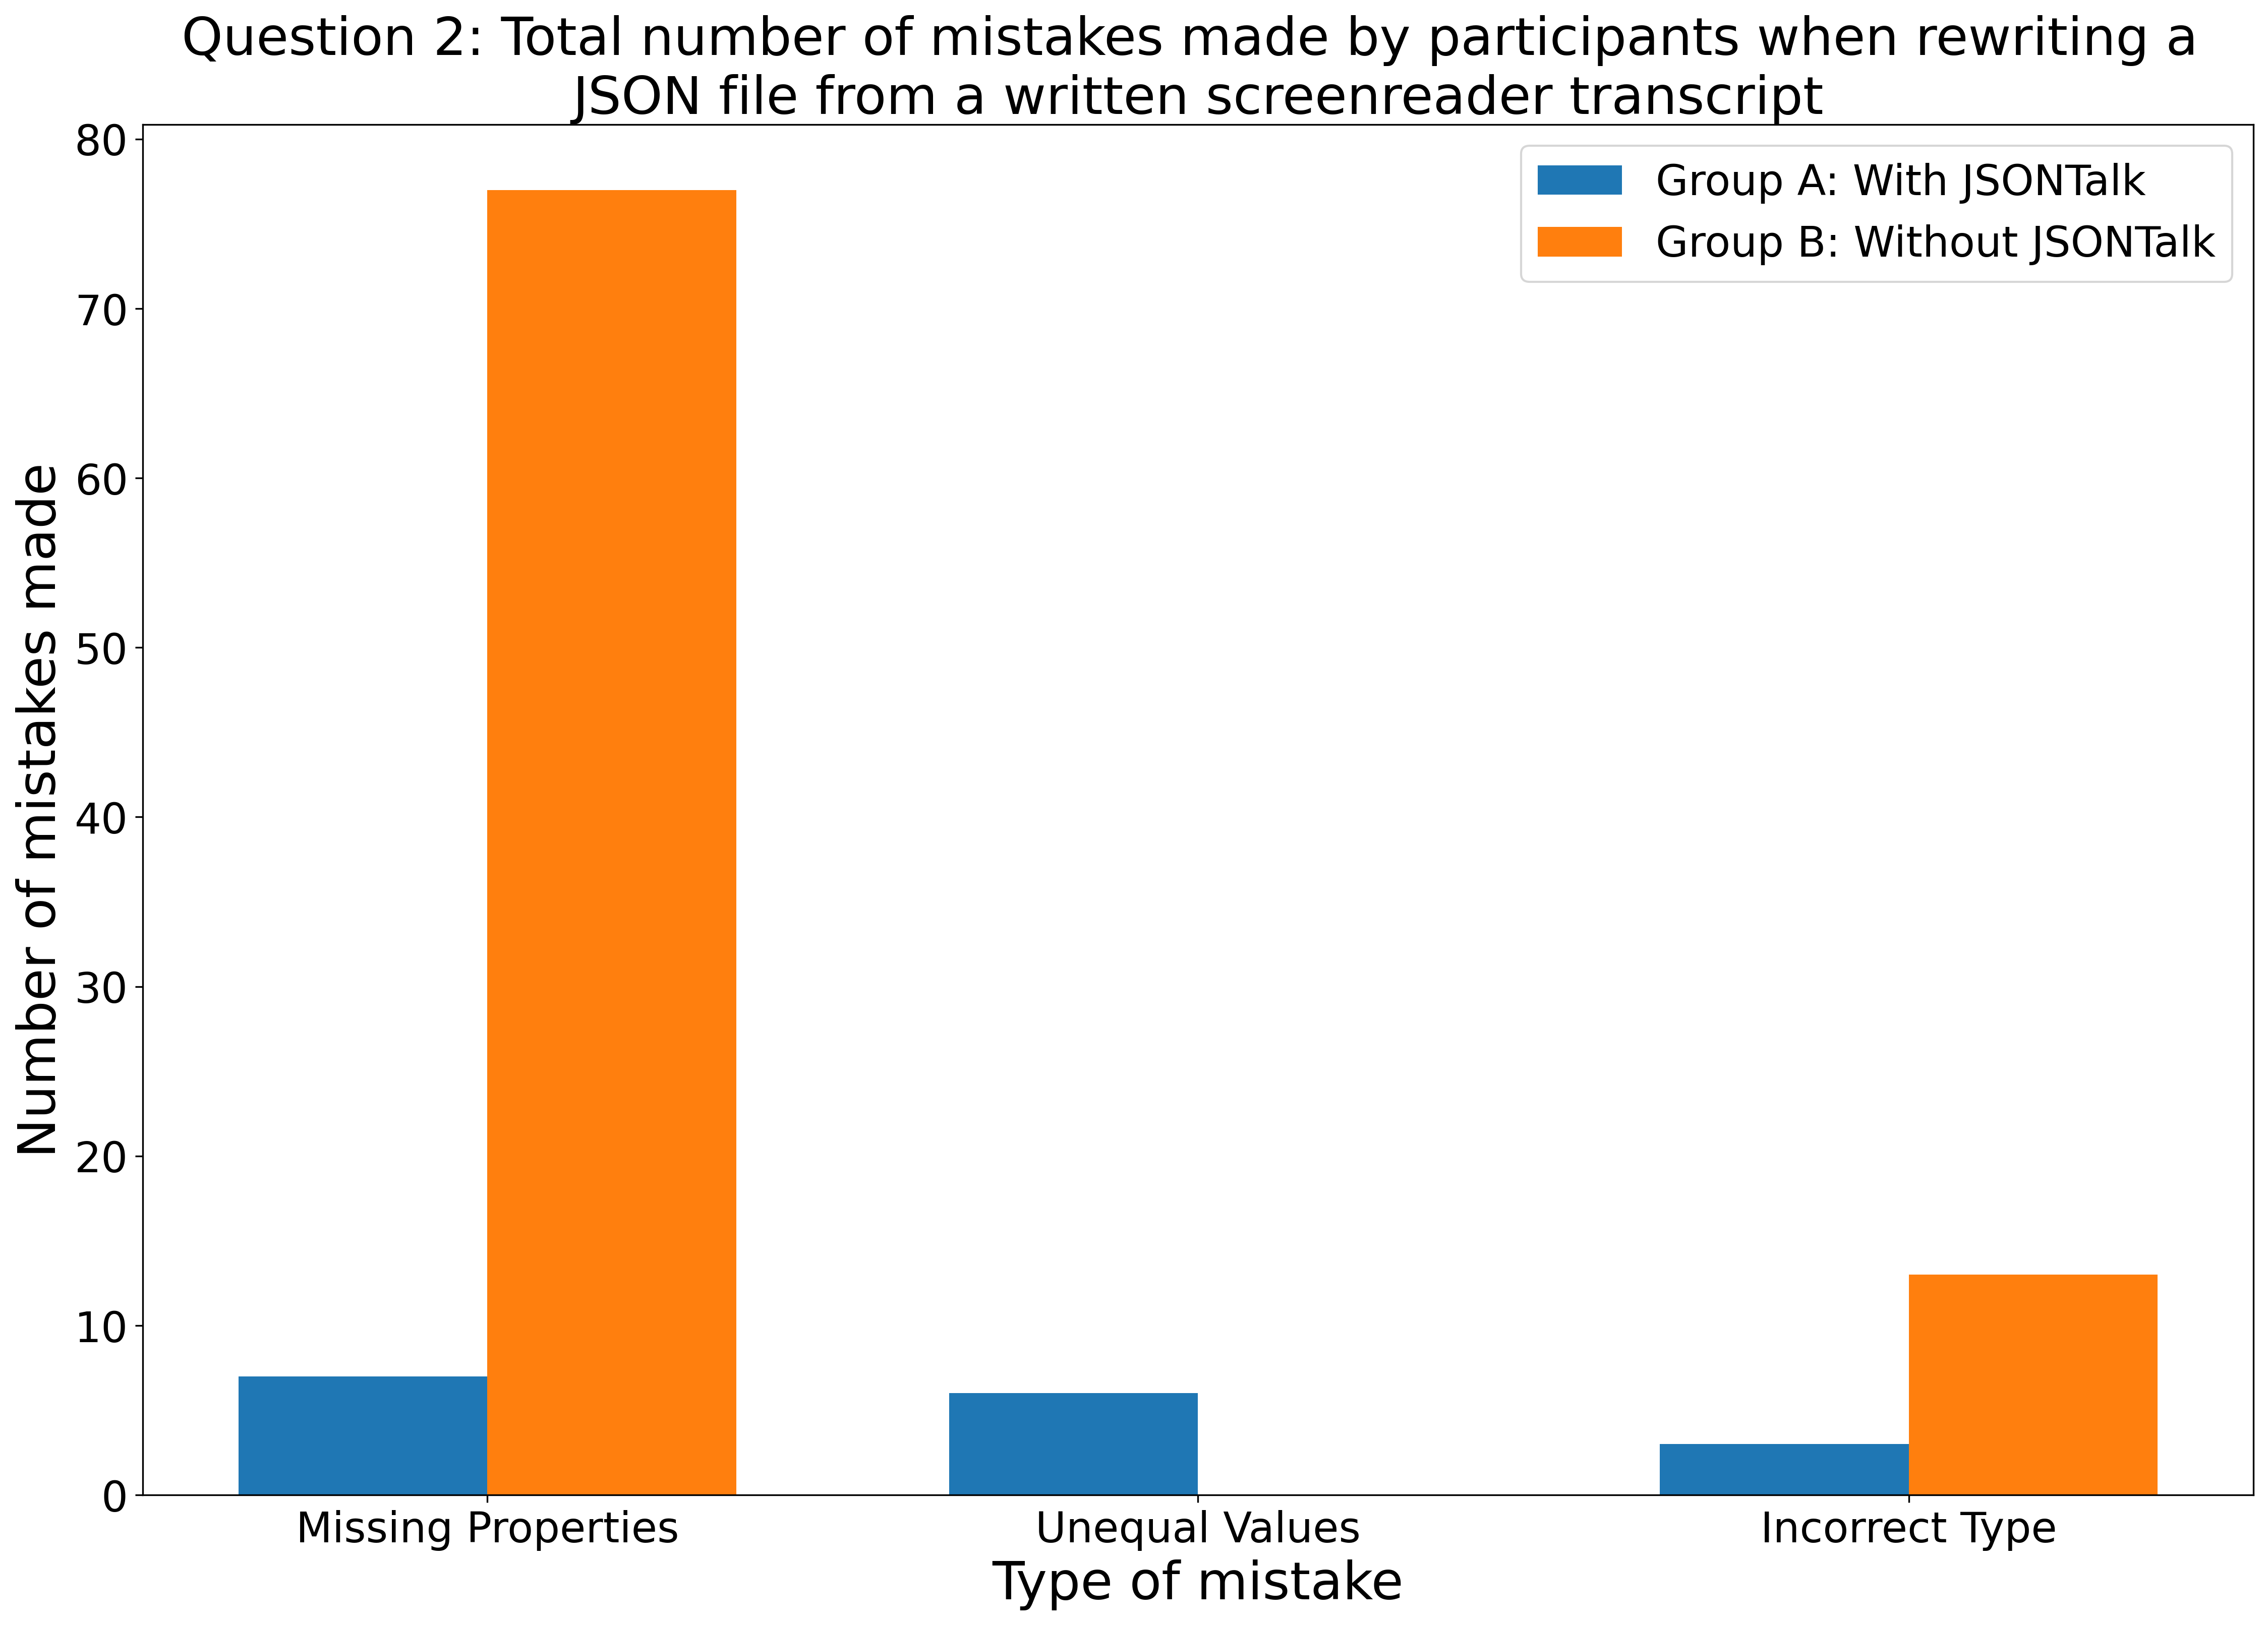
\includegraphics[width=\textwidth]{dissertation/images/Evaluation results/Question 2_ Total number of mistakes made by participants when rewriting a _JSON file from a written screenreader transcript.png}
        \caption{}
        \label{fig:q2graph_mistakes}

    \end{subfigure}
    \begin{subfigure}{0.49\textwidth}
        
        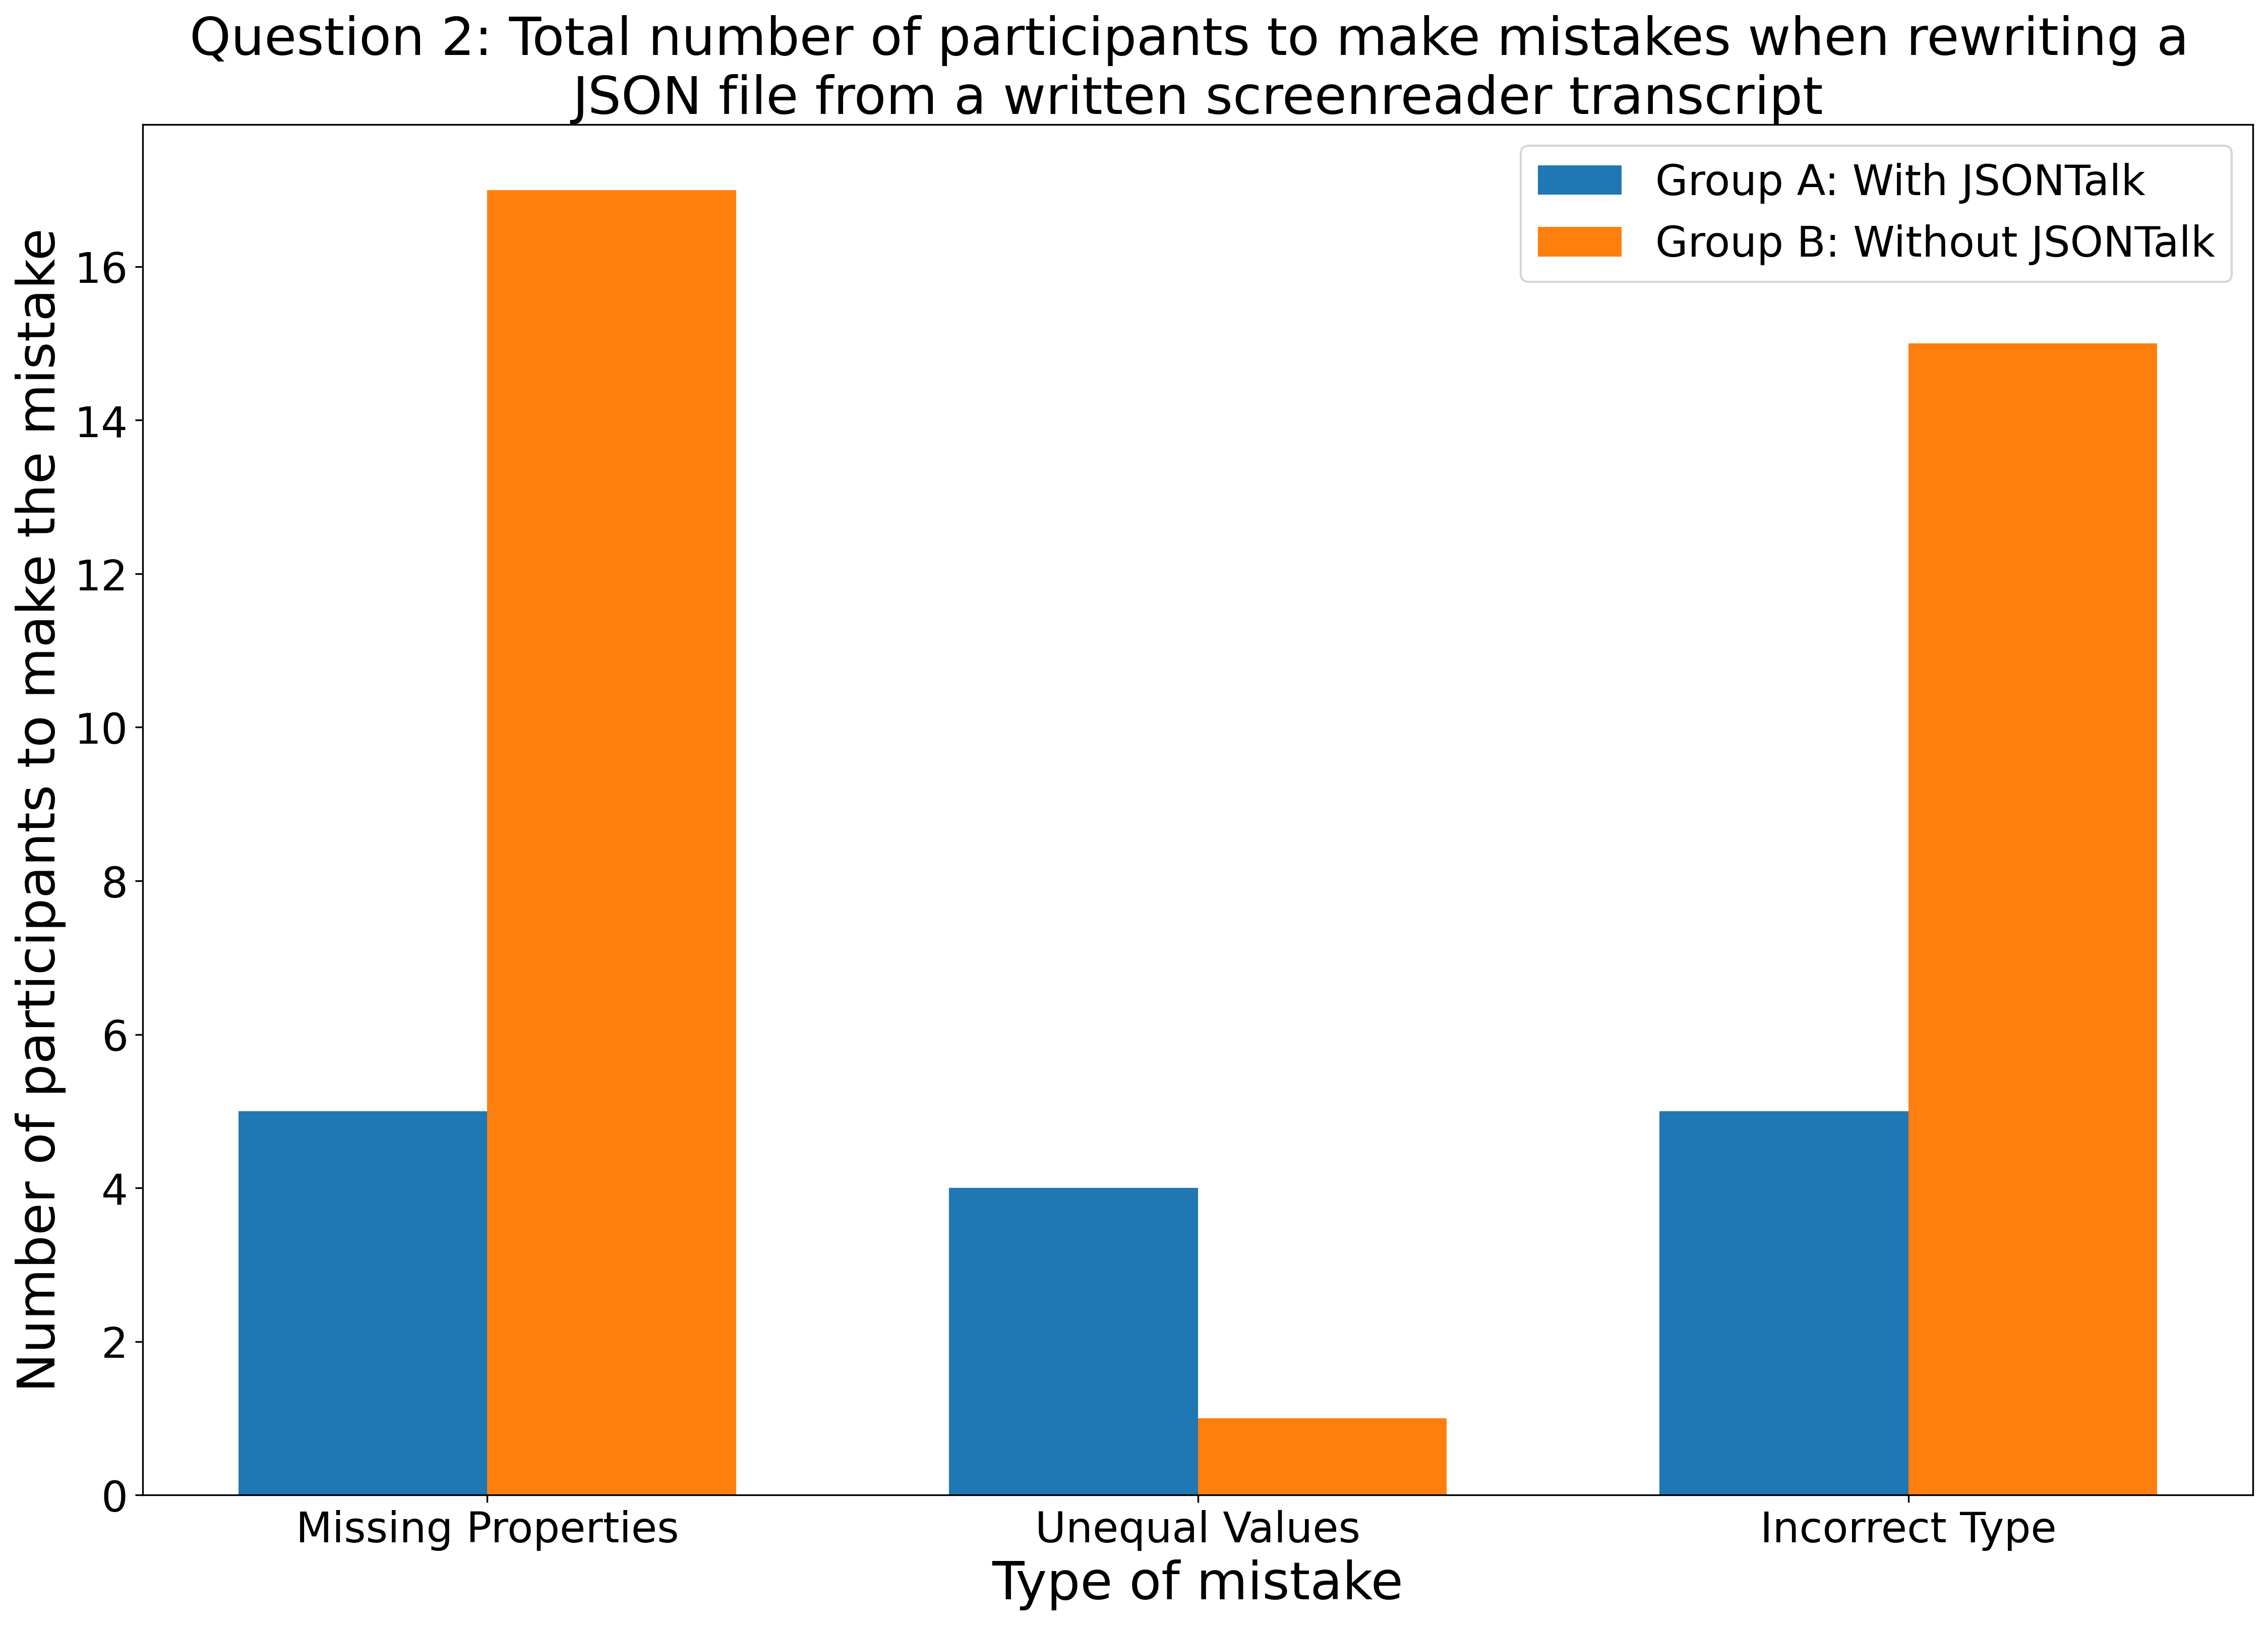
\includegraphics[width=\textwidth]{dissertation/images/Evaluation results/Question 2_ Total number of participants to make mistakes when rewriting a _JSON file from a written screenreader transcript.png}
        \caption{}
        \label{fig:q2graph_participants}

    \end{subfigure}

    \caption{}
\end{figure}

%\begin{wrapfigure}{L}{0.45\textwidth}
 %   \centering
  %  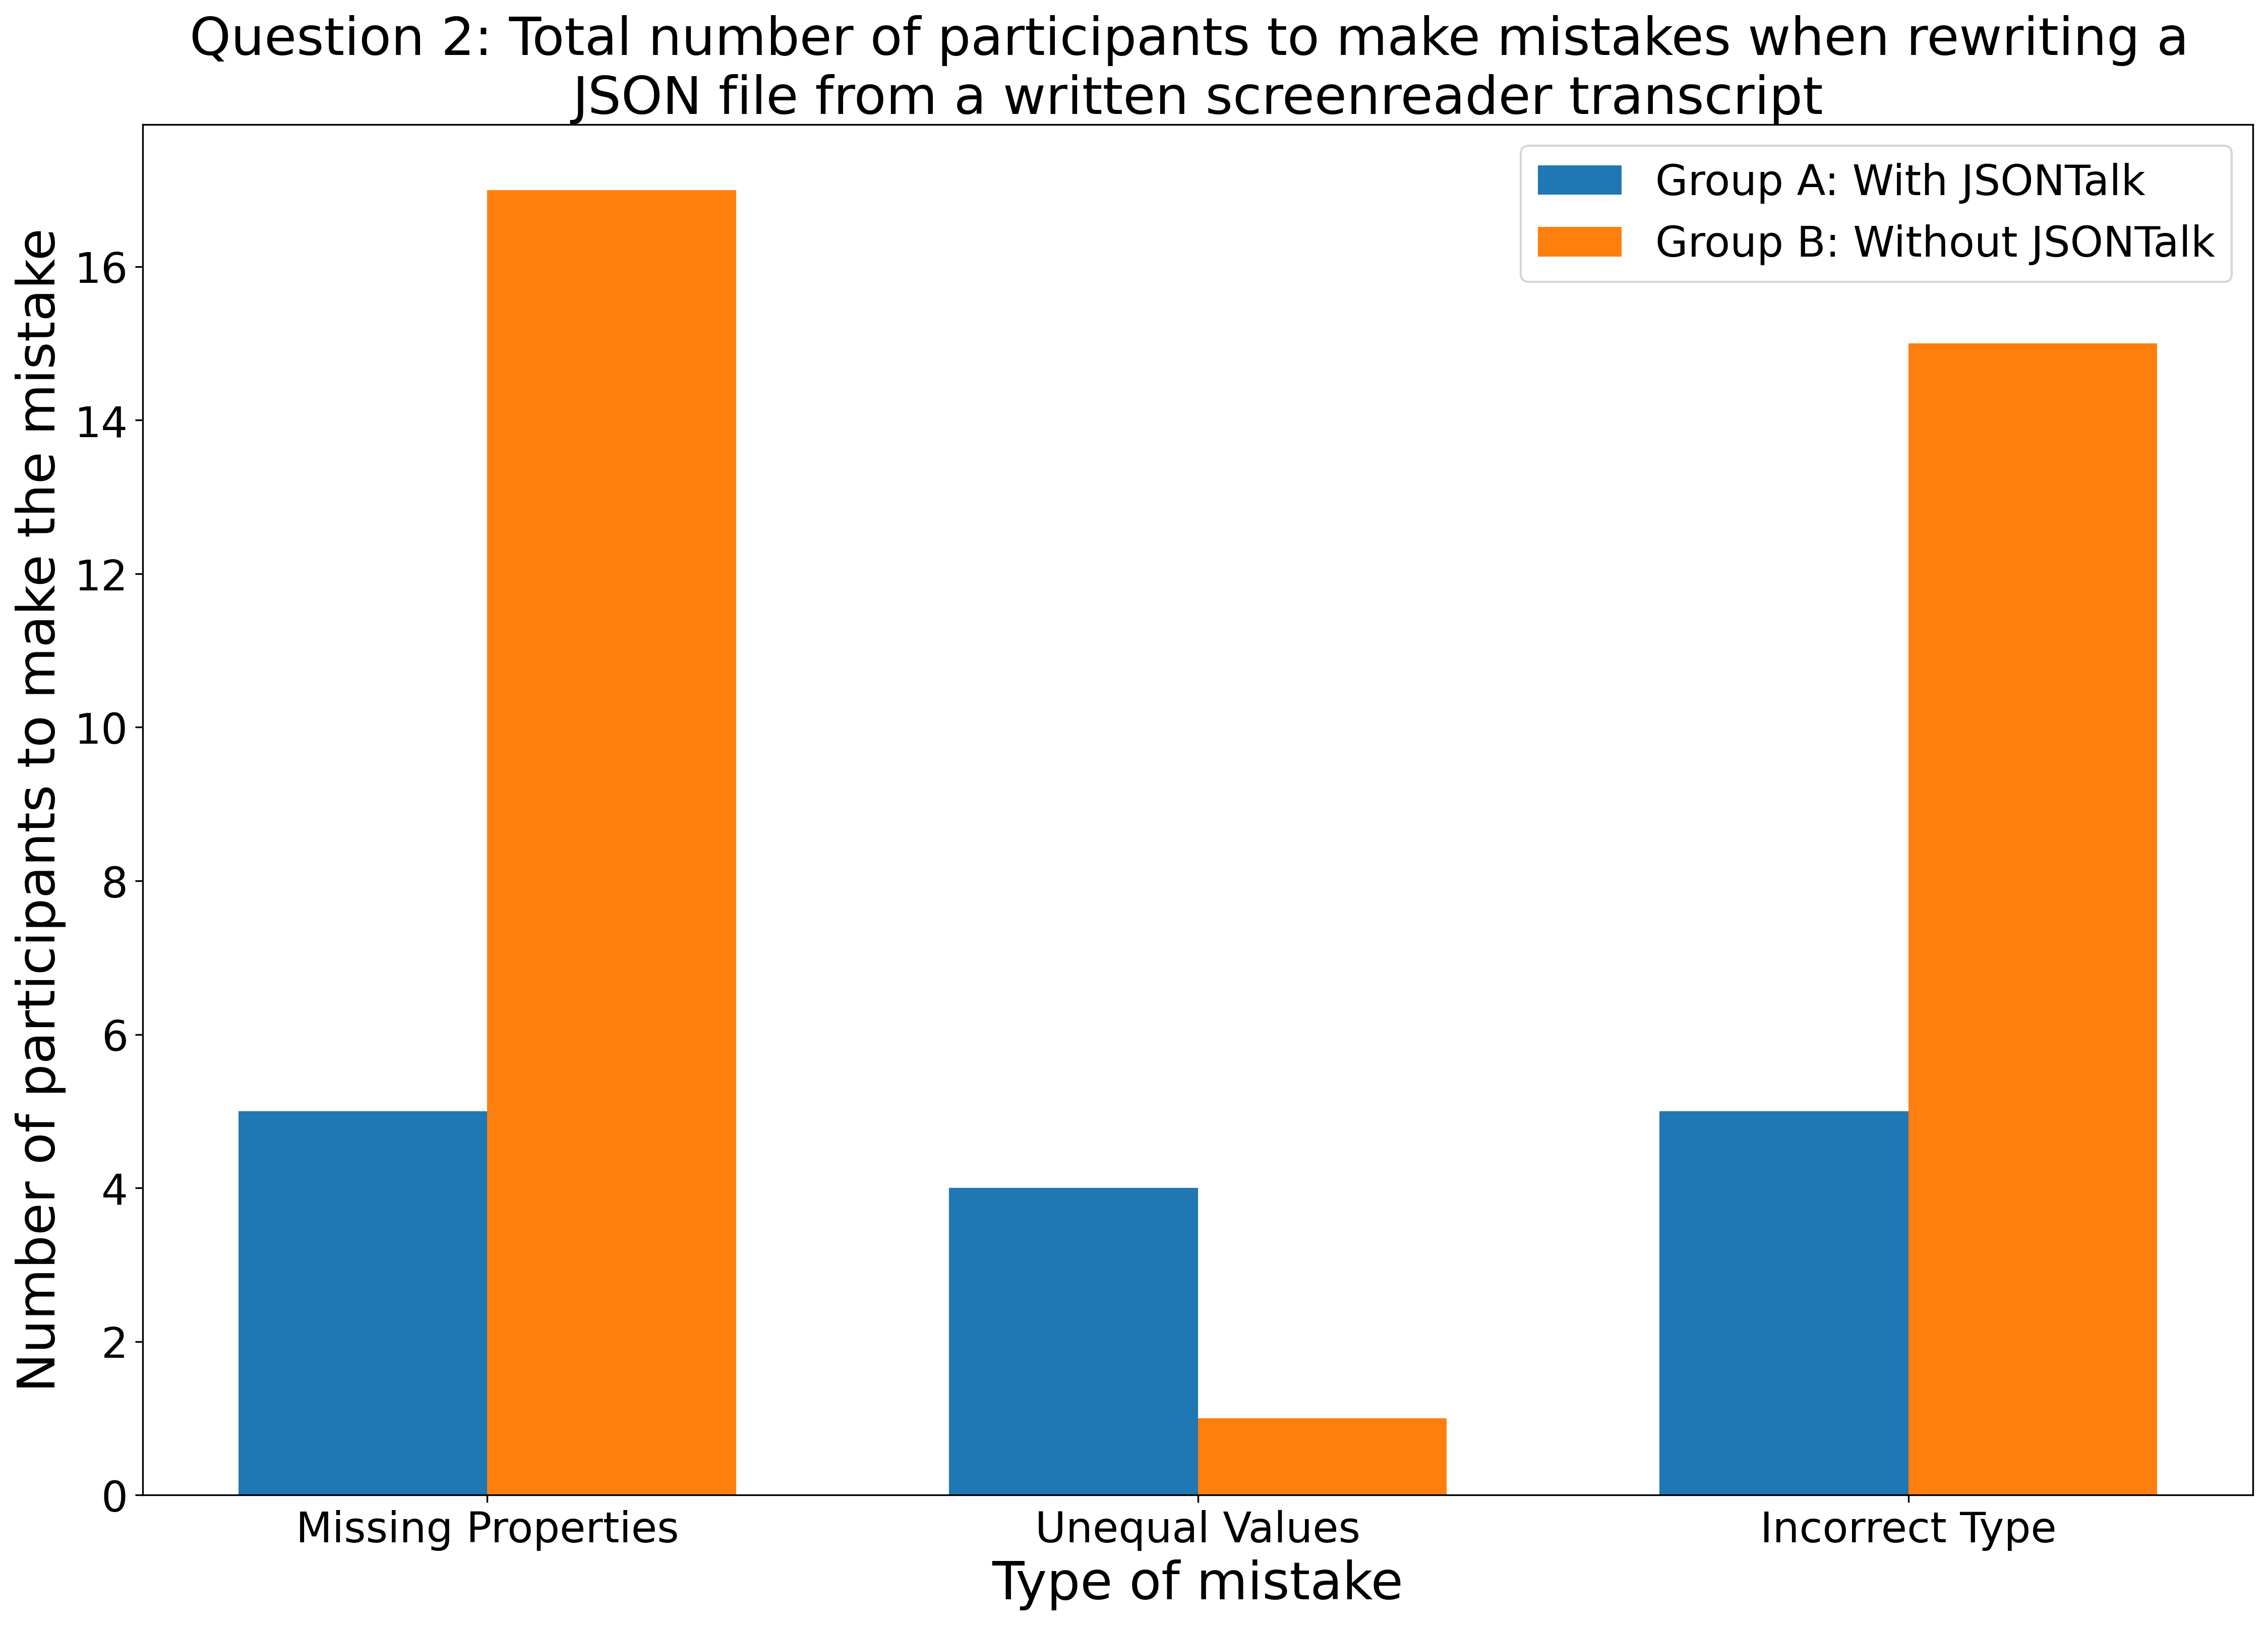
\includegraphics[width=0.45\textwidth]{dissertation/images/Evaluation results/Question 2_ Total number of participants to make mistakes when rewriting a _JSON file from a written screenreader transcript.png}
    %\caption{}
%\end{wrapfigure}

Figure \ref{fig:q2graph_mistakes} shows the total number of errors made in each category by each group when rewriting the JSON file. Overall, 16 mistakes were observed across the answers given by group A and 90 errors were observed in the answers given by group B. 

A Chi-square test was conducted on the results to determine whether there is a significant difference in the overall number of errors when rewriting the JSON file with and without the JSONTalk tool. The test yielded a p-value lower than 0.05, indicating that the difference observed is statistically significant. Therefore, we can conclude that the tool does have a significant effect on participants' interpretation of the semantic meaning of a JSON file. 


\begin{table}
\small
\centering
\centerline{
\begin{tabular}{p{0.22\textwidth}|p{0.8\textwidth}}
\multicolumn{2}{c}{\textbf{Question 2 number of mistakes statistical analysis}} \\ \hline
{Null hypothesis} & There is no significant difference between the total mistakes made by participants when rewriting a JSON file from a screen reader transcript using or not using the JSONTalk tool. \\ \hline
{Chi-square statistic} &  36.9129\\ \hline
{P-value} &  0.0000\\ \hline
{Degrees of freedom} &  2\\ \hline
{Conclusion} & \textbf{Null hypothesis rejected }\\ 
\end{tabular}
}
\end{table}



\paragraph{Number of participants to make mistakes}\hfill



Figure \ref{fig:q2graph_participants} shows the percentage of participants in each group who made mistakes in each category when rewriting the JSON file. Overall, 27.78\% of the participants in group A made a mistake when rewriting the file, while 68.18\% of the participants in group B made a mistake. 

A Chi-square test was conducted on the results to determine whether there is a significant difference in the proportion of incorrect participants when rewriting the JSON file with and without the JSONTalk tool. The test yielded a p-value lower than 0.05, indicating that the difference observed is statistically significant. Therefore, we can conclude that the tool does have a significant effect on participants' interpretation of the semantic meaning of a JSON file.


\begin{table}
\centering
\centerline{
\small
\begin{tabular}{p{0.22\textwidth}|p{0.8\textwidth}}
\multicolumn{2}{c}{\textbf{Question 2 number of participants to make a mistake statistical analysis}} \\ \hline
{Null hypothesis} & There is no significant difference between the number of participants to make a mistake when rewriting a JSON file from a screen reader transcript using or not using the JSONTalk tool.\\ \hline
{Chi-square statistic} &  9.5707\\ \hline
{P-value} &  0.0084\\ \hline
{Degrees of freedom} &  2\\ \hline
{Conclusion} & \textbf{Null hypothesis rejected} \\ 
\end{tabular}
}
\end{table} 

\paragraph{Question 2 Timing}\hfill

We recorded the time it took the participants to complete Question 1, both with and without the tool. Group A took an average of 383.48 seconds to complete Question 1, and group B took an average of 468.99 seconds to complete the question. 

To determine whether there is a statistically significant difference between the completion times, we performed a Mann-Whitney U test on the results. The test produced a p-value lower than 0.05, indicating that the observed difference is statistically significant. Therefore, we conclude that the tool has a significant effect on the completion time of Question 2, compared to completing the question without the tool.


\begin{table}[ht]
\small
\centering
\centerline{
\begin{tabular}{p{0.22\textwidth}|p{0.8\textwidth}}
\multicolumn{2}{c}{\textbf{Question 2 overall timing statistical analysis}} \\ \hline
{Null hypothesis} & There is no significant difference between the time it takes for participants to rewrite a JSON file from a written screen reader transcript using or not using the JSONTalk tool. \\ \hline
{Mann-Whitney U test} & 121.5000 \\ \hline
{P-value} & 0.02295 \\ \hline
{Effect size (Cohen's d)} & -0.7165 \\ \hline
{Conclusion} & \textbf{Null hypothesis rejected} \\ 
\end{tabular}
}
\end{table}


%\begin{figure}
 %   \centering
  %  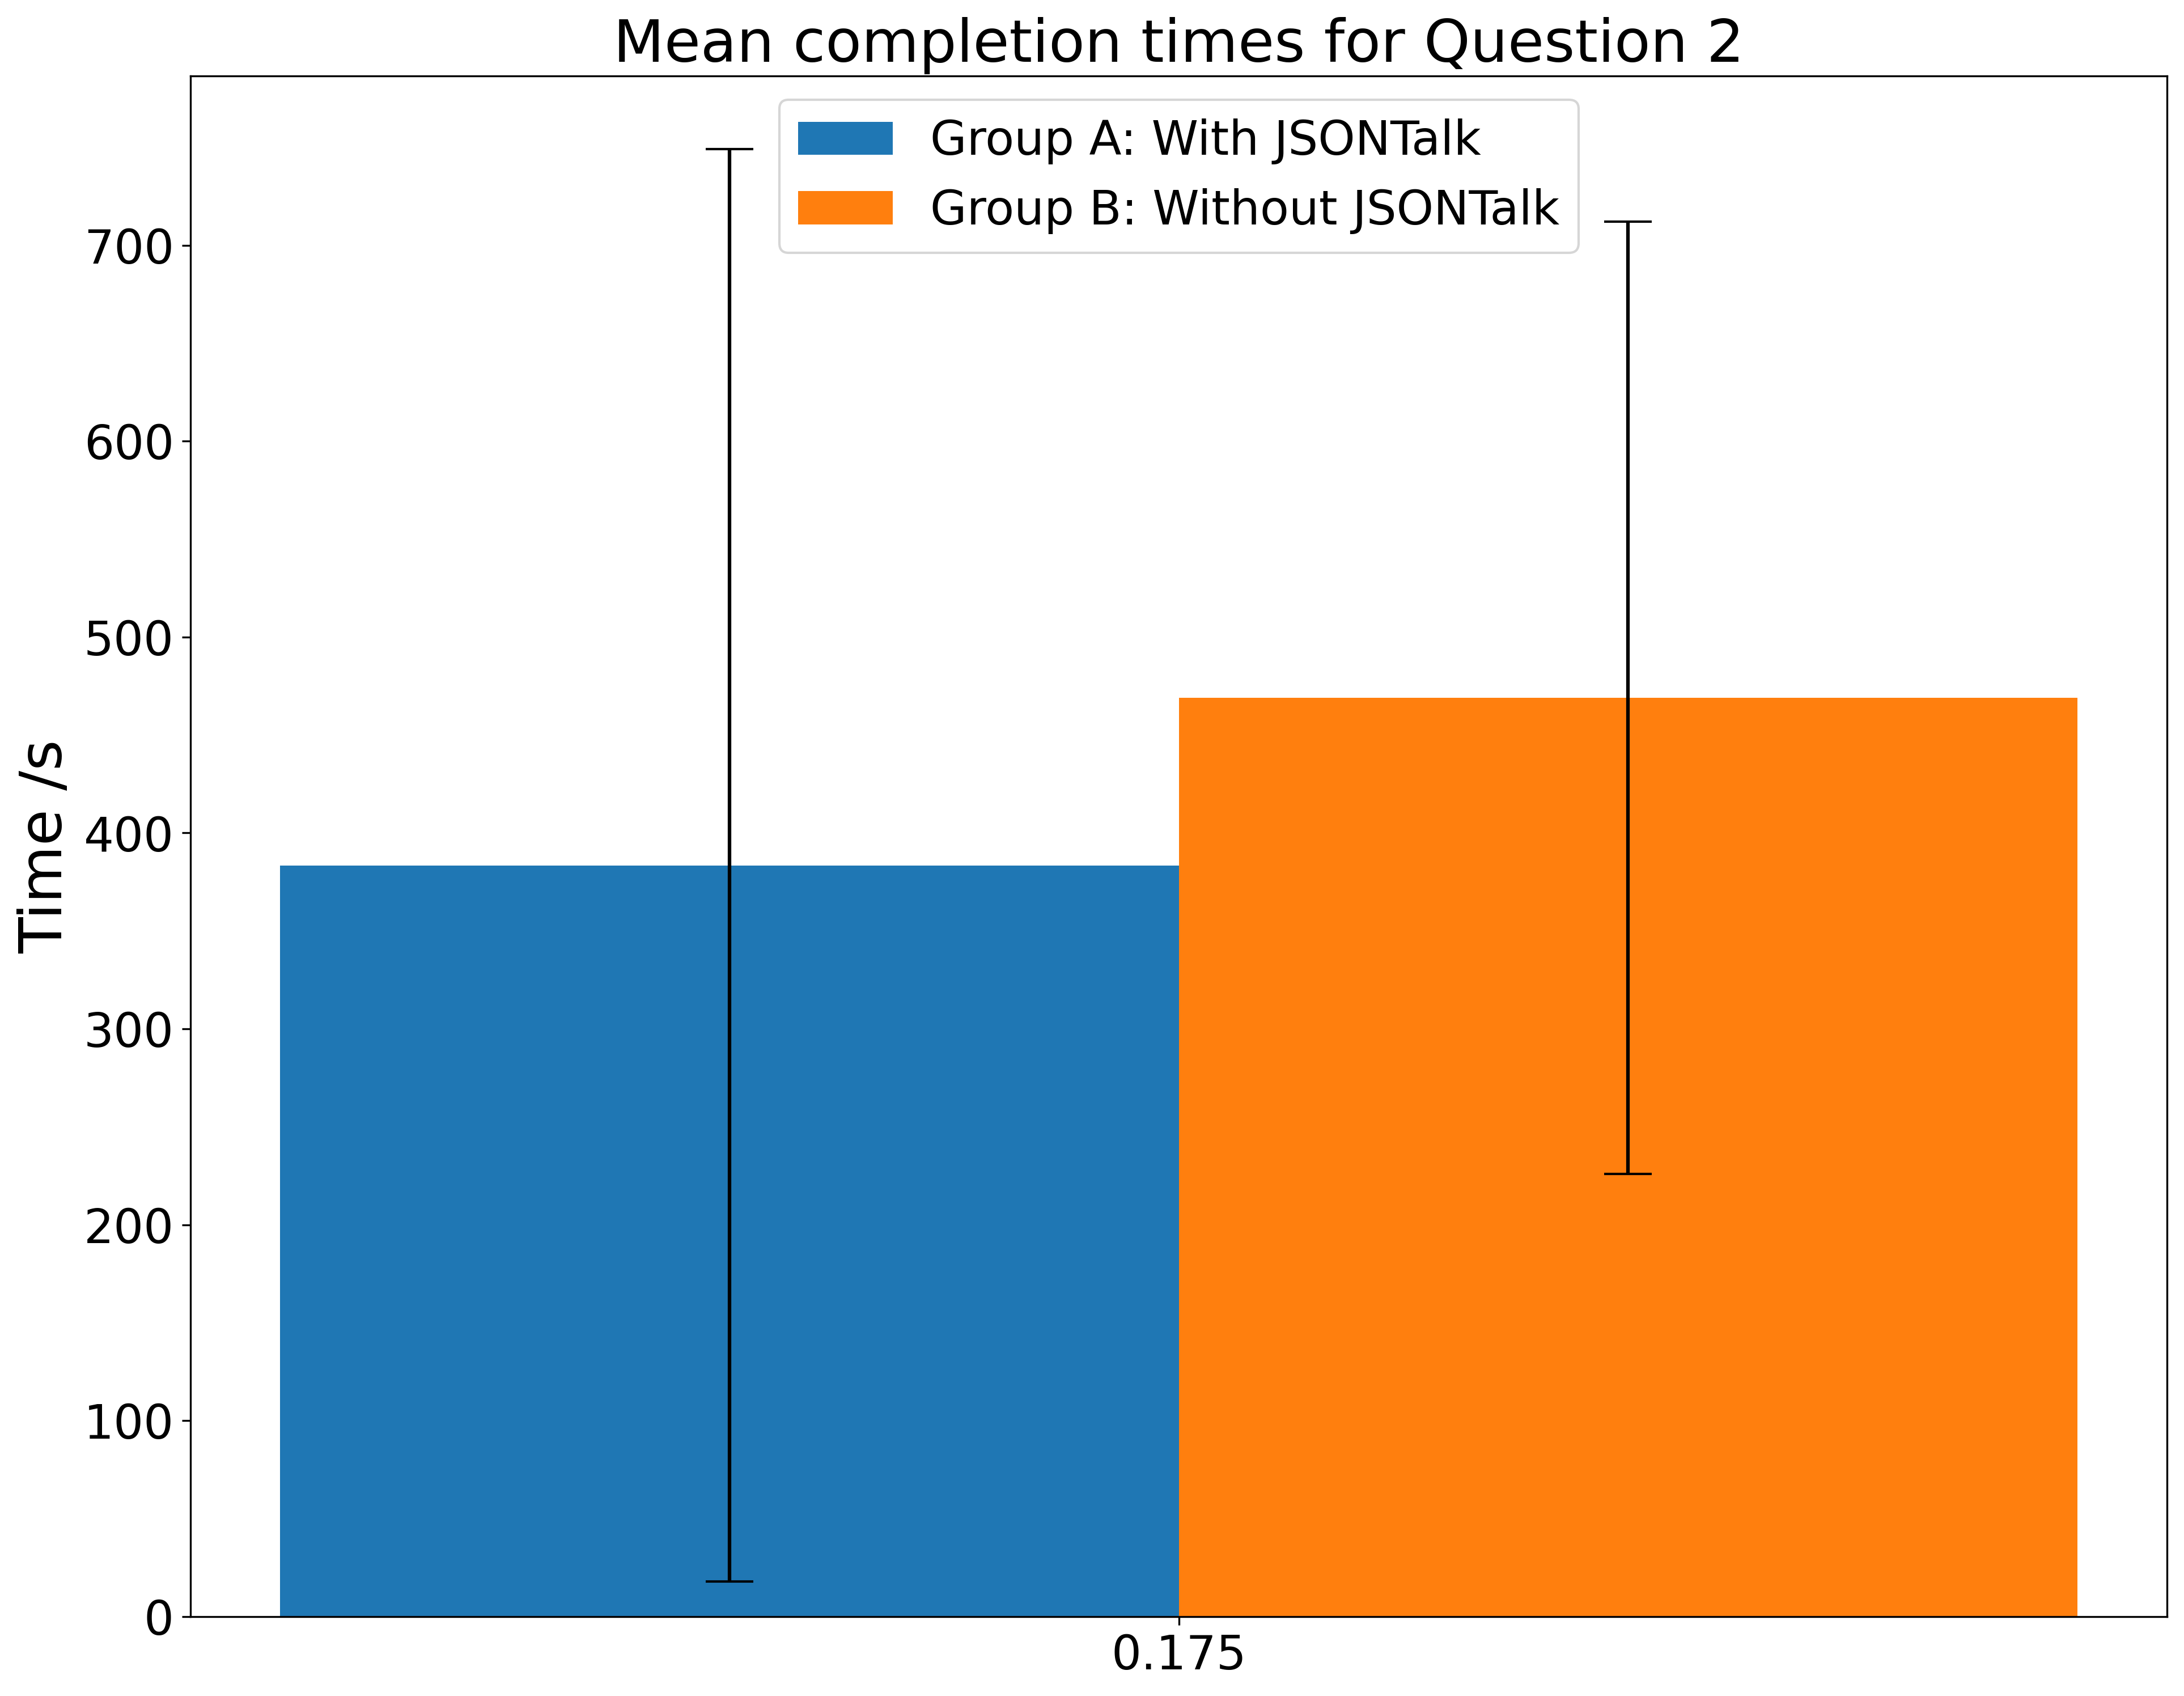
\includegraphics[width=0.8\textwidth]{dissertation/images/Evaluation results/Mean completion times for Question 2.png}
   % \caption{}
   % \label{fig:q1graph}
%\end{figure}

\subsubsection{Question 3: Answering a depth and structure question based on a JSON file being read by a screen reader}\hfill

\begin{wrapfigure}{L}{0.45\textwidth}
    \centering
    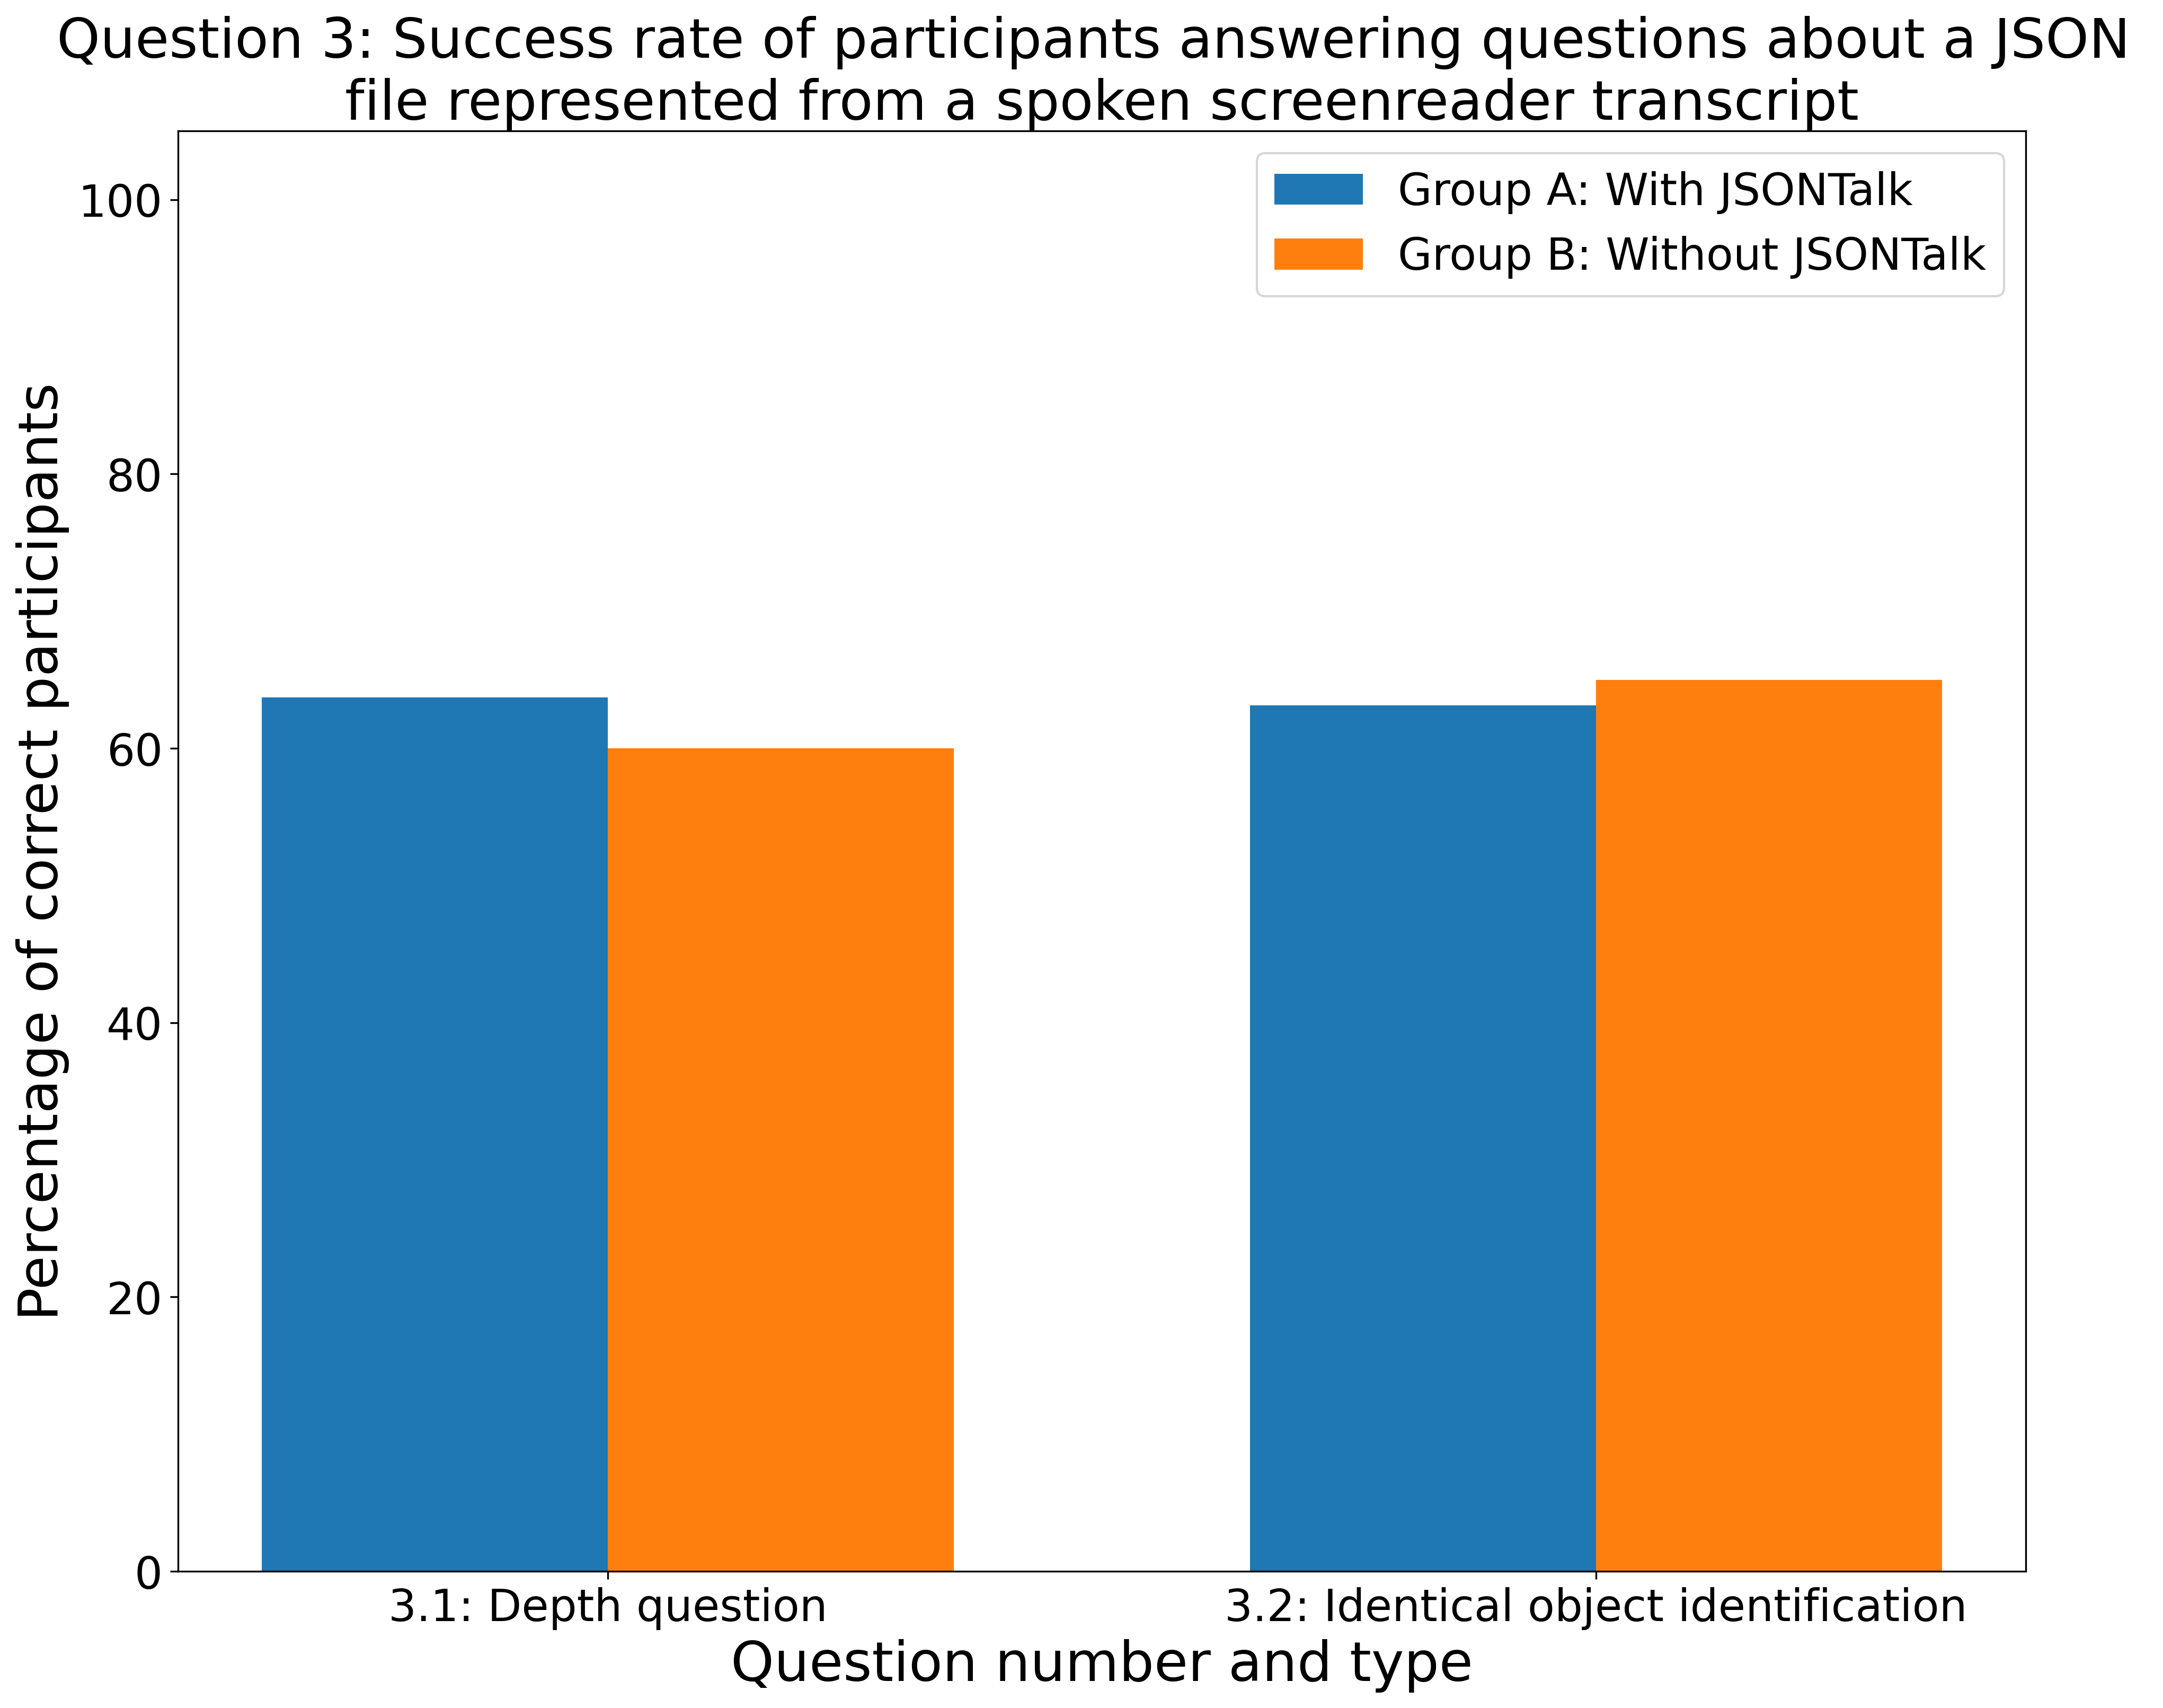
\includegraphics[width=0.45\textwidth]{dissertation/images/Evaluation results/Question 3_ Success rate of participants answering questions about a JSON _file represented from a spoken screenreader transcript.png}
    \caption{}
    \label{fig:q3graph}
\end{wrapfigure}

Our objective in this question was to investigate the impact of the text-to-speech feature in a tool and its effectiveness as an audio-based interface. It is important to note that our study was conducted with sighted participants who had no prior experience in hearing structured data aurally. To assess the participants' comprehension, we presented an audio clip of a screen reader reading a JSON file for Question 3. Group A participants were instructed to use the read-aloud functionality of the JSONTalk tool without referring to the written command line output. As the study was conducted remotely, we relied on the honesty of the participants to adhere to this instruction. Participants were subsequently asked a depth-based question and an identical object identification question about the file. 

\paragraph{Question 3.1: Question based on depth}\hfill

The first part asked participants to determine the depth of object "y" if object "x" was located at depth 1. In the same way as we did with the results of question 1, the data was then processed by encoding each answer as correct or incorrect. We found that 64.71\% of the participants in group A answered correctly, while 60.00\% of the participants in group B answered correctly.

A Chi-square test was conducted on the results to determine whether there is a significant difference in participants' ability to answer a depth question correctly with or without the use of the JSONTalk tool. The test yielded a p-value greater than 0.05, indicating that the difference observed is statistically significant. Therefore, we can conclude that there is not a significant difference between the two groups in their ability to answer the depth question.


\begin{table}[ht]
\small
\centering
\centerline{
\begin{tabular}{p{0.22\textwidth}|p{0.8\textwidth}}
\multicolumn{2}{c}{\textbf{Question 3.1 statistical analysis}} \\ \hline
{Null hypothesis} & There is no significant difference between the number of participants to answer a depth based question correctly using or not using the JSONTalk tool based on a spoken screen reader transcript\\ \hline
{Chi-square statistic} &  0.0458\\ \hline
{P-value} &  0.8305\\ \hline
{Degrees of freedom} &  1\\ \hline
{Conclusion} & \textbf{Null hypothesis accepted} \\ 
\end{tabular}
}
\end{table}


\paragraph{Question 3.2: Identical object identification}\hfill

The second part required participants to identify whether any objects in the underlying JSON file had identical structures. To clarify the second question, the participants were given an explanation of what it means for objects to have identical structures. For this, participants were required to choose one of 3 options (yes, no, unsure), and during processing, the data was encoded as correct, incorrect, or unsure. We found that 63.16\% of the participants in group A answered this correctly, 21.05\% were unsure, and 15.79\% were incorrect. 
In group B, 65.00\% of the participants were correct, 30.00\% were unsure and 5.00\% were incorrect. 

A Chi-square test was conducted on the results to determine whether there is a significant difference in participants' ability to answer an object structure question correctly with or without the use of the JSONTalk tool. The test yielded a p-value higher than 0.05, indicating that the difference observed is not statistically significant. Therefore, we can conclude that the tool does not have a significant effect on participants' ability to identify the presence of identical objects.


\begin{table}[ht]
\small
\centering
\centerline{
\begin{tabular}{p{0.22\textwidth}|p{0.8\textwidth}}
\multicolumn{2}{c}{\textbf{Question 3.2 statistical analysis}} \\ \hline
{Null hypothesis} & There is no significant difference between the number of participants to correctly identify identical objects within a JSON file using or not using the JSONTalk tool based on a spoken screen reader transcript \\ \hline
{Chi-square statistic} &  1.4153\\ \hline
{P-value} &  0.4928\\ \hline
{Degrees of freedom} &  2\\ \hline
{Conclusion} & \textbf{Null hypothesis accepted} \\ 
\end{tabular}
}
\end{table}



\paragraph{Question 3 Timing}\hfill

We recorded the time it took the participants to complete Question 1, both with and without the tool. Group A took an average of 593.72 seconds to complete Question 1, and group B took an average of 1272.31 seconds to complete the question. 

To determine whether there is a statistically significant difference between the completion times, we performed a Mann-Whitney U test on the results. The test produced a p-value higher than 0.05, indicating that the observed difference is not statistically significant. Therefore, we conclude that the tool does not have a significant effect on the completion time of Question 3, compared to completing the question without the tool.


\begin{table}[ht]
\small
\centering
\centerline{
\begin{tabular}{p{0.22\textwidth}|p{0.8\textwidth}}
\multicolumn{2}{c}{\textbf{Question 3 overall timing statistical analysis}} \\ \hline
{Null hypothesis} & There is no significant difference between the time it takes participants to answer 2 questions about a JSON file using or not using the JSONTalk tool \\ \hline
{Mann-Whitney U test} &  175.0000\\ \hline
{P-value} & 0.6837 \\ \hline
{Effect size (Cohen's d)} & -0.1350 \\ \hline
{Conclusion} & \textbf{Null hypothesis accepted} \\ 
\end{tabular}
}
\end{table}



%\begin{figure}
%    \centering
 %   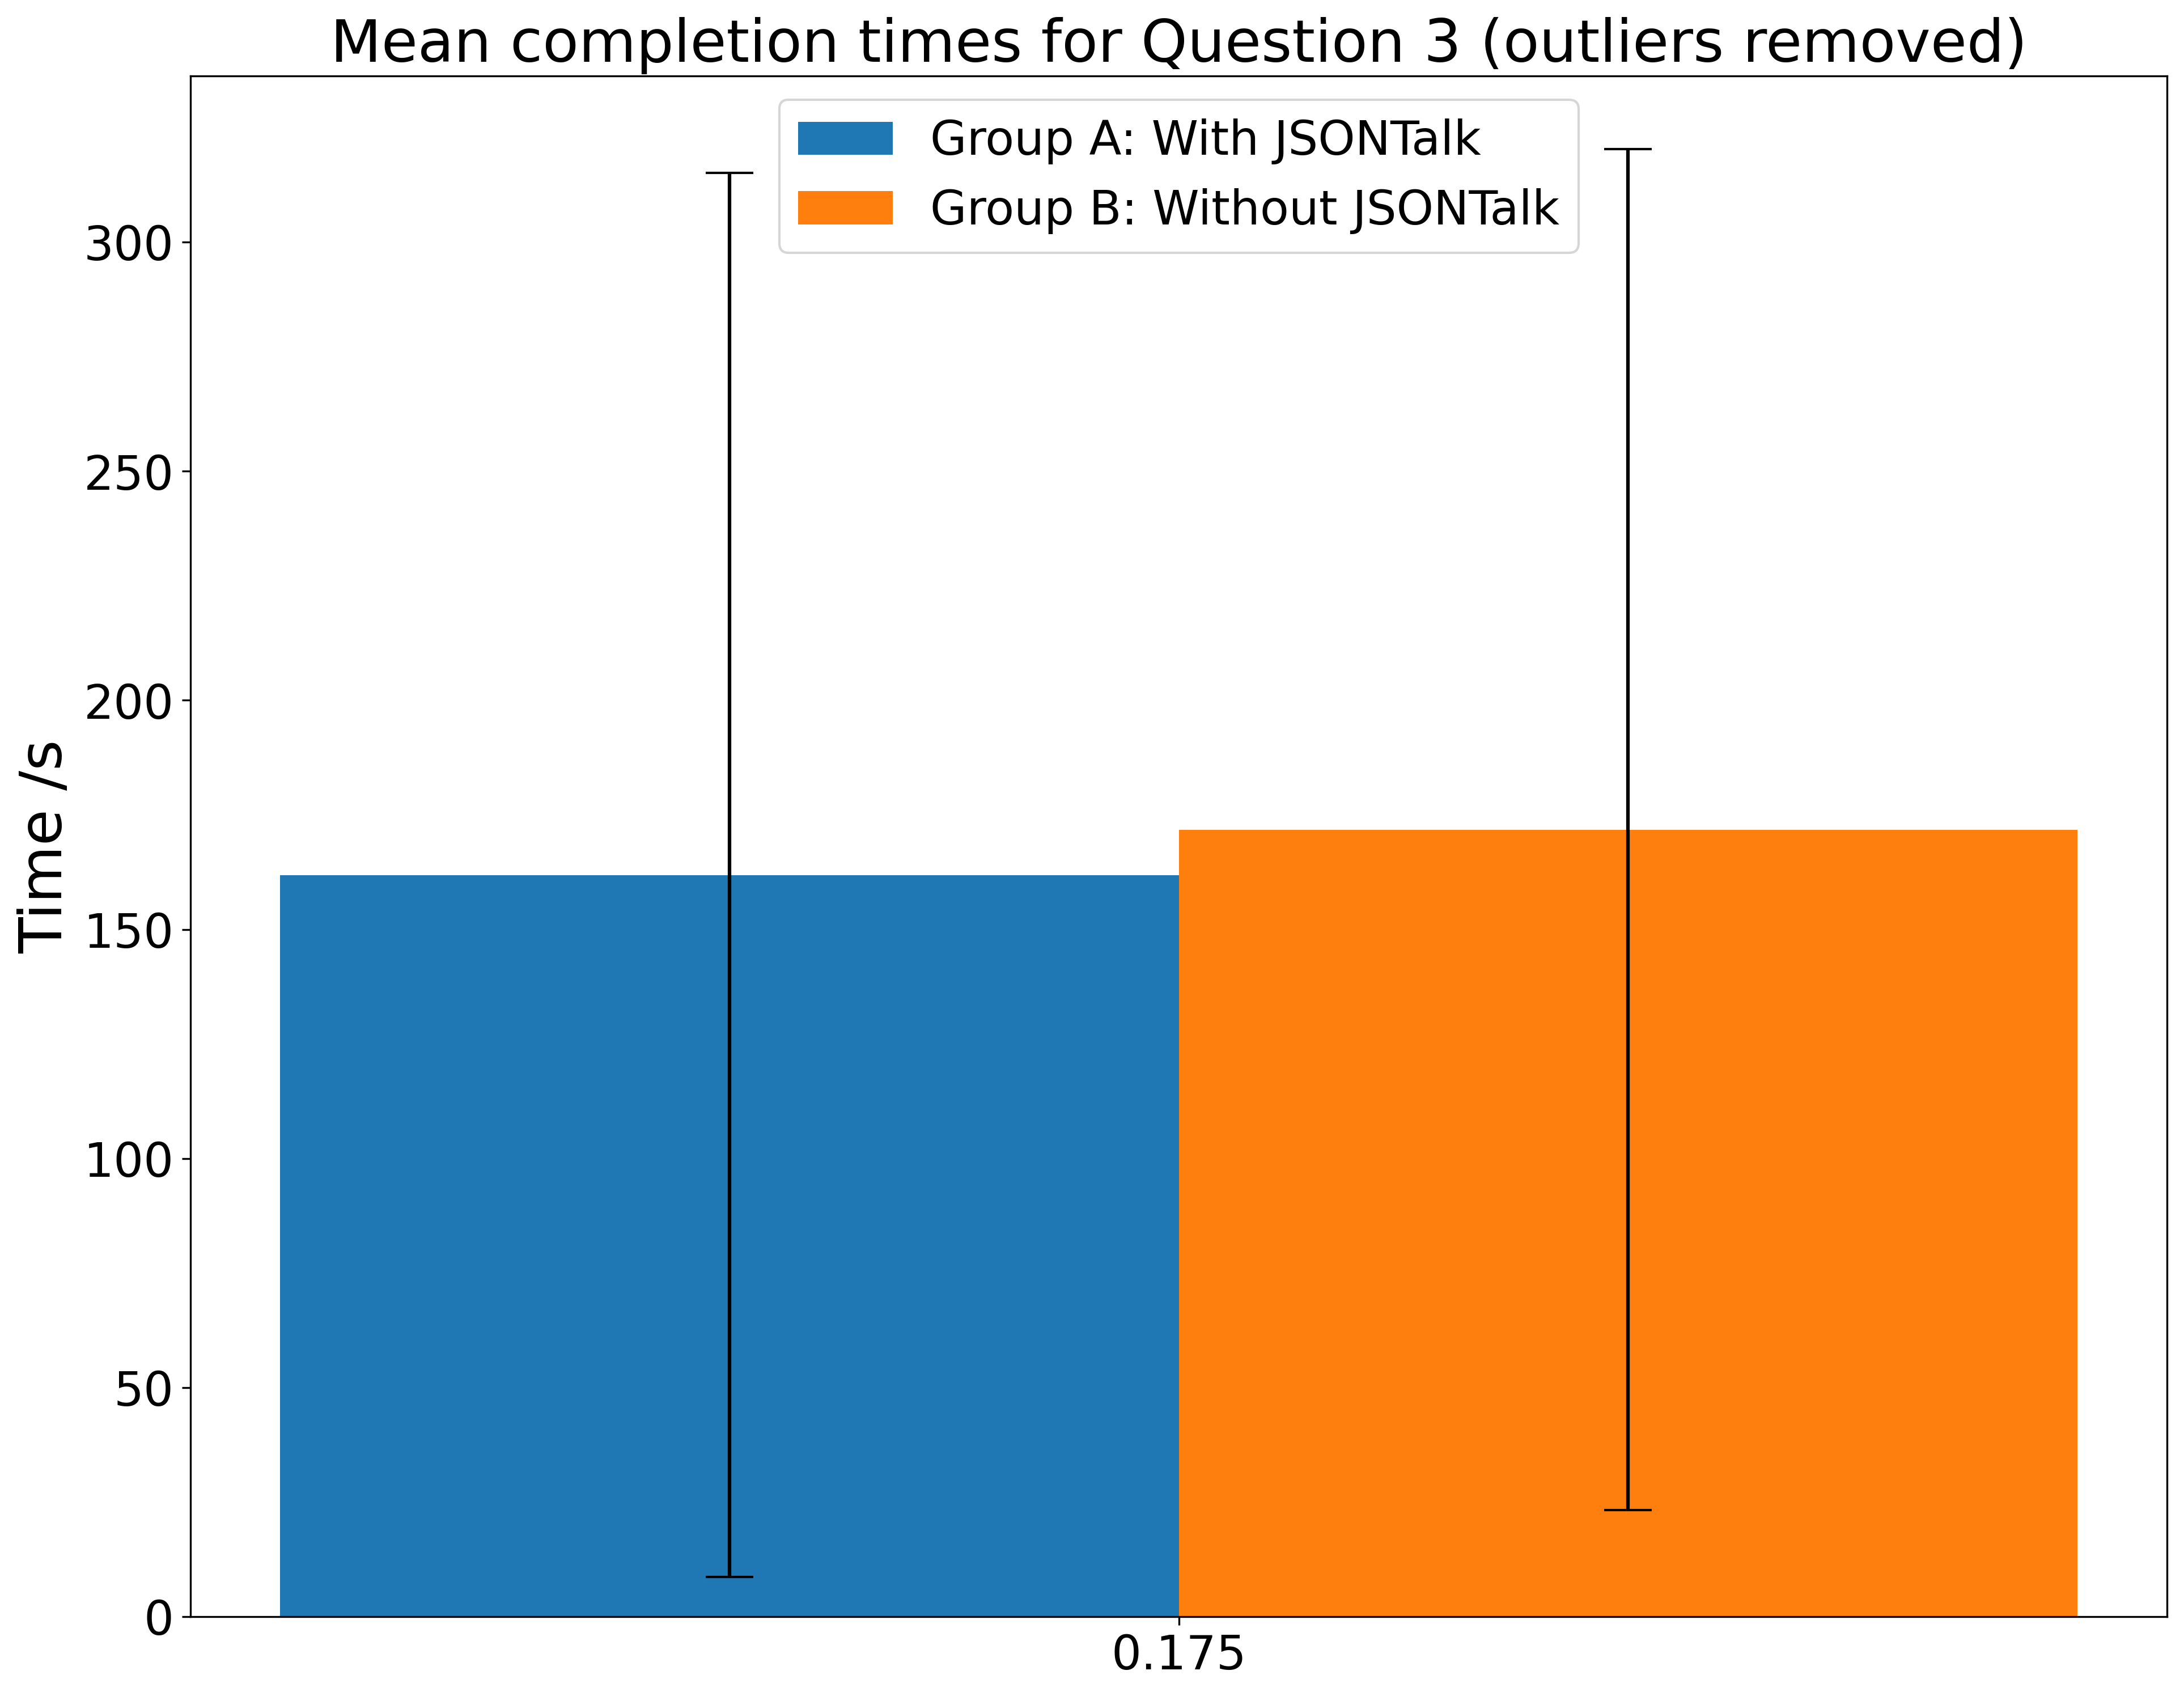
\includegraphics[width=0.8\textwidth]{dissertation/images/Evaluation results/Mean completion times for Question 3 (outliers removed).png}
  %  \caption{}
   % \label{fig:q1graph}
%\end{figure}

\subsubsection{Question 4: Usability Questionnaire}\hfill

The final stage of the study involved asking participants from Group A the System Usability Scale questionnaire \cite{brooke2013sus}. The System Usability Scale (SUS) is a widely used questionnaire that measures the perceived usability of a system or product. It consists of 10 statements that participants rate on a 5-point Likert scale ranging from "strongly disagree" to "strongly agree." The SUS score is calculated by converting the ratings to a standardised scale and then averaging them. The resulting score ranges from 0 to 100, with higher scores indicating better usability. We obtained a mean SUS score of 62.5. 62.5 indicates that the JSONTalk tool is of a moderately usable level and does not fulfil our non-functional requirement of a usability score of over 75.  However, it is important to note that the SUS score is just one aspect of usability and does not provide a comprehensive evaluation of the system.

\section{Discussion}
\subsection{Evaluation limitations}

This evaluation only involved sighted participants. Although this detail was mitigated by presenting participants screen reader transcripts of JSON files instead of actual JSON files, the evaluation would have yielded more meaningful results about JSONTalk as a tool for VI programmers if it directly involved VI programmers. 

The sighted programmers recruited also reported having never used screen readers before and not having been used to hearing code or structured data spoken out loud. This meant that Question 3 presented a challenge to both groups of participants, regardless of whether they used a spoken description of the JSON file from the screen reader excerpt or the JSONTalk read-aloud functionality. This challenge was reflected in the results, with the average completion time for question 3 much higher than that of questions 1 and 2, which used written JSON representations. We found that there was no significant difference between the participants' completion time or accuracy rate for question 3 between group A and group B. The unfamiliarity of spoken structured data representation may have been a factor in this.

We also recognise that there is learning effect in the study, and in order to make it easier for participants to complete the study, we presented the questions in the same order to all participants, building up from simple questions about a written JSON representation, rewriting the original JSON file from written JSON representation and finally answering some questions about spoken representation of a JSON file. However, randomising the order for participants to answer the questions would have reduced the learning effect across questions and produced more representative results. However, as we did not directly compare the results across different questions, this is not a huge issue.

Although the between-subject design of the experiment reduced the carryover learning effect between the two conditions, a higher number of participants was required to yield representative results. Participants were randomly assigned to either group upon recruitment; however, an initial recruitment complete with demographic and JSON familiarity questions could have taken place.  

\subsection{Evaluation conclusions}

As discussed in the limitation section above, all participants were unfamiliar with spoken descriptions of structured data, which may have influenced the results of Question 3 such that there was no significant difference between groups A and B. Considering the results of questions 1 and 2, we can conclude the following:
\begin{itemize}
    \item The JSONTalk tool can help users better understand the depth of elements within JSON files compared to just using a screen reader.
    \item  More work needs to be done for the JSONTalk tool to give users a better overview of identical objects within JSON files.
    \item  The JSONTalk tool allows users to decipher a JSON file more quickly and accurately compared to users using a screen reader.
\end{itemize}



\chapter{Exploratory study: ChatGPT descriptions}

%With the rising popularity of Generative AI models such as GPT-3.5, and as mentioned in Section \ref{section:code_summary} there is potential to harness generative AI for the task of generating natural language descriptions of structured data formats such as JSON. We explored the potential of this possibility using ChatGPT \cite{chatgpt}.  Although the primary focus of this project was on the development and evaluation of the JSONTalk tool, the rise in popularity of widespread generative AI usage in the middle of the project prompted us to explore its potential for generating descriptions of JSON data. The release of ChatGPT in November 2022 has raised so many interesting questions on how generative AI can be harnessed for wide variety of different purposes in many different fields. Hence, it is important to investigate this option as a viable alternative to the JSONTalk tool, given its wide availability and popularity. A browser-based tool that allows users to analyse files and generate custom descriptions of code or structured data to fit their specific needs can be highly valuable.

Since the release of ChatGPT \cite{chatgpt} in November 2022 (midway through this project), there has been a dramatic surge in the widespread use of generative AI. ChatGPT is built upon OpenAI's large language model GPT-3.5,  There is great potential to harness a tool such as ChatGPT to generate high quality natural language descriptions of structured data formats such as JSON. Although the primary focus of this project has been the development and evaluation of the JSONTalk tool, it is important to investigate generative AI as a viable alternative to the JSONTalk tool. ChatGPT is a great tool, as it is currently free and browser based, meaning users do not have to purchase or download anything to use it. The accessibility and versatility of this tool, which would allow users to generate descriptions of JSON files to fit their needs, are highly valuable. 

\section{Methodology}

To accomplish this, we used the files from the user study and instructed ChatGPT to generate descriptions for each file using the prompt "Describe this JSON file: <JSON file>". Each prompt was sent in a separate "chat" window, to ensure that the conditions were constant. We recorded the first response given by ChatGPT following each prompt, and made observations based on the descriptions obtained. From this experiment, we aim to develop a set of research questions that may inform further research in this area.


\section{Results}

\subsection{Descriptions generated by ChatGPT}

The descriptions for each JSON file can be viewed in Appendix \ref{appenidix:chatGPT}.

\subsection{Observations}

The following observations can be made from the ChatGPT generated descriptions.

\subsubsection{Same conditions, different description:}

Despite executing the same prompt under the same conditions, the descriptions are all quite different. Description A is very detailed and specific, focussing on the structure and data contained within the JSON file. It provides a comprehensive overview of each book object, describing the properties and values within each one. Description B, on the other hand, takes a more general approach to describing JSON files. It provides an explanation of what JSON is and what it is used for, as well as a broad overview of the key-value pairs contained within the file. Description C strikes a balance between the two, providing both a general overview of the file's structure and a more detailed look at its contents. It introduces the main properties of the file and explains their purpose, before diving into the specific details of the "items" property.

The fact that ChatGPT generated three distinct descriptions for three different JSON files using the same prompt demonstrates the versatility and adaptability of generative AI like ChatGPT. More context aware descriptions based on the content of JSON files may be beneficial in providing users more relevant details. In particular, providing less information for a simple JSON file, vs. providing more detailed explanation of a more complicated JSON file.

On the other hand, consistency in descriptions of JSON files can be beneficial for screen reader users who rely on such descriptions to understand the structure and content of the file. Having a consistent format and style of description across different JSON files can help users with visual impairments quickly and easily understand the information contained in the file, especially if they are already familiar with the structure and properties of JSON objects. 

This raises an interesting research question: \textit{\textbf{“Do users favour consistent descriptions or summarisations when using code or structured text summary tools?”}}. Understanding user preferences can help improve the design of code or structured text summary tools, making them more effective and user-friendly.

\subsubsection{Inference:}

The three descriptions each provide an inference about the meaning or purpose of the JSON file, which the JSONTalk tool is unable to generate. Further research could explore whether such inferences are valuable to users of code or structured data summarising tools, and identify specific use cases where they may be useful.

This inference highlights a key difference between generative AI and predefined parse and description generation methods such as those used by the JSONTalk tool. JSON files are typically used within a larger context, such as a NoSQL database or RESTful API, and programmers rarely examine them in isolation. As a result, the context of the JSON file may already provide sufficient information for programmers to infer its purpose. Without this contextual information, the descriptions produced by generative AI can make a false inference about the purpose of a JSON file. This could mislead users and lead to wrong development decisions based on inaccurate information.

From this observation we raise the following research question: 
\textit{\textbf{"Are inferences about the purpose of code or data meaningful to users of code or structured data summarising tools?"}}

\subsubsection{Accuracy: } 

All three descriptions correctly depict the JSON files provided to ChatGPT without any errors. Nevertheless, it is important to note that generating accurate responses using generative AI cannot be guaranteed with 100\% certainty, as such AI models do not operate on a fixed set of rules. The inherent nature of generative AI makes it challenging to ensure complete accuracy. From this observation, we have developed a research question: \textit{\textbf{"How can we validate the accuracy of descriptions produced by generative AI?"}}. A tool for structured data or code descriptions which uses generative AI could have an integrating validation framework to assess the accuracy of descriptions before they are provided to the end user; however, further research would need to take place to develop a more robust idea of what this might look like. Furthermore, training a large language model, such as ChatGPT, on the specific task of code or structured data description is likely to improve accuracy.

\subsubsection{Length:}

When comparing the descriptions of the files produced by ChatGPT with the descriptions produced by JSONTalk, the ChatGPT generated descriptions are comparatively longer. For example, the JSONTalk description for file A is 105 words long, whilst the ChatGPT description for file A is 132 words long. The ChatGPT descriptions generated for the given files all contain an introductory sentence about the JSON data format. This information is redundant for some users seeking a quick overview of a JSON document when they already know what JSON is. This may be especially problematic for the time-constrained user persona detailed in section \ref{subsection: personas}, as they may not want to sift through unnecessary information. On the other hand, a short JSON introduction may be beneficial for the Novice Programmer user persona, detailed in section \ref{subsection: personas}. 

\subsubsection{Customisability:} One of the primary benefits of ChatGPT versus JSONTalk is the complete customisability of the description that can be produced by ChatGPT. Users can request JSON descriptions of variety of different tones, levels of detail, and even languages. The opportunities for customisation using ChatGPT far outweigh the opportunities for customisation using JSONTalk. 

\subsection{Discussion}

%This experiment has raised more questions than it has answered. To address these questions, conducting a user study that involves descriptions generated by ChatGPT would be highly beneficial. In the context of generating textual descriptions of code and structured data to widen accessibility, the accessibility of ChatGPT as a tool needs to also be explored. Further research into prompt optimisation should also take place. 

Conducting a user study that involves descriptions generated by ChatGPT could be highly beneficial in addressing the questions raised by this experiment. Specifically, the study could shed light on the accessibility of ChatGPT as a tool to generate textual descriptions of code and structured data, and further research into prompt optimisation could also be explored.


%==================================================================================================================================
\chapter{Conclusion}  

%This project involved the exploration of several issues within computer science. One of the main themes and motivations for this project was to improve the accessibility of programming and software development for VI programmers. We surveyed and epxlored current accesibility barriers within computer science. We examined the tool kit available to VI porgrammers, ranging from general purpose assistive technology for any ytpe of VI computer use, to specific research and tools created to address very specific issues faced by VI porgrammers. 

\section{Project summary}

This project involved the exploration of accessibility, structured data parsing, structured text to natural language mapping, and the potential of generative AI as a code summary tool. We developed and evaluated a tool that generates natural language summaries of JSON files, which has potential to assist VI, time-constrained, and novice programmers. 

We conducted a comparative analysis of the challenges faced by VI programmers, time-constrained programmers, and novice programmers. Although each persona encounters unique obstacles to productivity, we discovered a common functionality that could help address their specific challenges.

For instance, VI programmers could benefit from a more accessible and comprehensive textual description of the code's structure and content. Assistive technologies often constrain VI programmers, making it challenging to interact with the code or programming tools. Therefore, a textual description that is compatible with assistive technology and provides additional structural and contextual information could help address the code skimming and reading challenges faced by VI programmers.

Time-constrained programmers would benefit from a tool that provides a quick overview of the file's contents. A short and straightforward textual description could help them save time and understand the structure and contents of the JSON file more quickly.

Similarly, novice programmers may lack the syntax knowledge required for easy JSON reading. Therefore, a human-readable description of the file could help them understand the file more effectively.

Although we recognised that the JSON summarising tool could benefit time-constrained and novice programmers, we primarily focused on developing the JSONTalk tool as a tool for VI programmers. Our background research concentrated on the challenges faced by VI programmers and the current tools available to them. Furthermore, we evaluated the effectiveness of the JSONTalk tool by comparing it to existing screen reader representations of JSON files to understand how it could supplement unclear and challenging to understand screen reader representations.

Before development work, we conducted a thorough survey and analysis of the existing accessibility barriers within computer science. Our exploration encompassed an in-depth examination of the toolkit available to VI programmers. This toolkit ranged from general-purpose assistive technology for any type of VI computer use to specialised research and tools designed to address specific challenges faced by VI programmers.
We also surveyed state-of-the-art techniques currently used for code summarisation, with the purpose of automating documentation workflows, and pointed out the potential for use of these sophisticated techniques for assisting VI programmers getting an overview of code and structured data.

Based on the background research we conducted and analysis of current problems faced by VI programmers, we set to work developing a tool that generates natural language descriptions of JSON files. We further analysed the problems faced by VI, time-constrained and novice programmers and developed a set of functional and non-functional requirements for the JSONTalk tool. 

To implement the JSONTalk tool, we used ANTLR4 \cite{antlr4}, a parser generator tool, in combination with a formal JSON grammar definition. Lexing and parsing methods developed by ANTLR4, based on the grammar generated an AST from JSON files, which we traversed using the visitor design pattern \cite{hunt2013gang}. We built a secondary data structure using the visitor design pattern, and traversal of this allowed us to generate the description. Once the development of the tool was finished, we packaged it as a Jar file which can be run as a command line application by users.

We evaluated the performance of the tool with 40 sighted programmers, using a between subjects A/B test design, where subjects had to answer a series of questions about three different JSON file representations. One group was presented with screen reader JSON representations, while the other group was presented with the representations and was also allowed to use the JSONTalk tool to generate descriptions of the underlying JSON files. We found that the tool can help users better understand the depth of elements within JSON files, compared to using a screen reader (this addresses the issue of context when code reading which VI programmers face). We also found that users asked to reproduce the underlying JSON files from the representation did so quicker and more accurately using the JSONTalk tool compared to without using the tool. Our study also revealed that more work could be done to draw users' attention to repeated object structures.

With the rise of generative AI, we also performed an exploratory study of using ChatGPT to generate descriptions of the JSON files. We made and categorised the observations made when comparing the descriptions generated by ChatGPT to the descriptions generated by the JSONTalk tool. From the set of observations, we were able to formulate a set of research questions that could be addressed in future work related to the use of generative AI as a code summarising tool and as a tool to improve computing accessibility for VI programmers.

\section{Limitations}

\subsection{JSONTalk limitations}

The user study results revealed that there is still work to be done to improve the JSONTalk tool's ability to inform users about the structure of objects. Specifically, the study found that objects with identical structures should be highlighted more prominently to help users identify similarities and differences. Furthermore, the tool received a below average usability score from the SUS questionnaire, indicating that improvements need to be made to enhance the overall user experience.

One potential step to improve the usability of the tool could be to fine-tune the help option with more informative descriptions. Furthermore, qualitative feedback from the user study highlighted user dissatisfaction with the voice used for the read-aloud functionality of JSONTalk. Therefore, conducting further evaluations, particularly with VI programmers, to obtain more detailed feedback and suggestions could be meaningful in identifying changes that need to be made to improve the usability of the tool.

It is important to recognise that while the usability feedback received from sighted programmers is useful, their perspective on usability may differ from that of VI programmers. For sighted users, usability is often focused on a well-developed user interface with appropriate visual cues. However, usability takes on a completely different nature when it comes to VI users, as the way they interact with systems is different. Therefore, it is critical to consider the needs and experiences of VI programmers in improving the usability of the JSONTalk tool.


\subsection{JSONTalk evaluation limitations}

The JSONTalk user study had a significant limitation in that it only involved sighted programmers. Although we attempted to simulate screen reader representations of JSON files to create a more representative tool use case, sighted programmers may not be accustomed to screen reader representations of JSON files at all. This could have resulted in a lack of familiarity and potential bias in the study's results, as the tool's effectiveness may differ between sighted and VI users.

In contrast, VI programmers (VI programmers) may have experience with JSON screen reader representations and interact with them in a completely different way, utilising command keys to interact with the content on screen. This difference in experience could result in varied opinions and use cases for the tool, which should be taken into account when evaluating its effectiveness.

Furthermore, our study only compared the JSONTalk tool descriptions to screen reader representations of JSON files, neglecting to compare it to other assistive technologies, such as refreshable braille displays, magnification, and high-contrast software. This limited our evaluation of the tool's effectiveness for a wide range of users, as different users may require different forms of assistive technology to access and interact with JSON files.

It is important to note that our results from the JSONTalk evaluation were not normally distributed, which may indicate that we did not receive enough responses to obtain fully representative data. This highlights the need for further research to fully assess the effectiveness and accessibility of the JSONTalk tool and to include a more diverse range of users with different levels of visual impairment and experience with assistive technology.

\subsection{Exploratory study limitations}

While making observations based on ChatGPT JSON descriptions, we could have expanded our exploratory study in the following ways:

\begin{itemize}
    \item Used a variety of different prompts: Using more prompts and comparing the descriptions generated across a different set of prompts could have given us further insight into prompt optimisation for generating JSON descriptions using prompt-based generative AI.
    \item Used more JSON files, in particular, more varied JSON files: Using a wider variety of JSON files would have given us further insight into how and why JSON descriptions vary.
    \item Used more generative AI models: We only conducted the exploratory study using ChatGPT, which is based on OpenAI's GPT-3.5 model. Exploring the descriptions generated by a variety of different models would have given us further insight into what makes a model suitable for describing JSON files. Looking at the training data and methods for different models would further inform this.
\end{itemize}

Furthermore, we recognised ChatGPT as a potential alternative to JSONTalk, incorporating ChatGPT generated JSON descriptions into the user study conducted to evaluate JSONTalk (i.e., conducting A/B/C tests in the form <no tool>/<jsonTalk>/<chatGPT>) would have allowed us to make more concrete conclusions on the effectiveness of ChatGPT for easier and faster understanding of JSON files.

To ensure ChatGPT is a valuable tool for VI programmers, it is crucial to evaluate its accessibility for VI users. If ChatGPT excels at generating JSON file descriptions but is not accessible to VI users, it undermines its usefulness as a summarising tool for this user group. Therefore, evaluating and addressing accessibility concerns is essential to ensure that ChatGPT can be a valuable asset to all programmers, including those with visual impairments.

\section{Future work}

Our work on the JSONTalk tool focused exclusively on speech-based descriptions of JSON files for VI programmers, using textual descriptions that can be read by screen readers or the tool's TTS functionality. However, previous research discussed in the background section of this dissertation has highlighted the potential for non-speech output modalities to enhance the nonvisual representation of code and structured data. To fully explore the capabilities of nonvisual JSON representation, future work should investigate the effectiveness of different nonspeech output modalities.

The use of only speech to represent JSON files provides only a superficial exploration of the possible output modalities available for non-visual representation. Some of the potential non-speech output modalities that could be investigated include:
\begin{itemize}
    \item Tactile output: This could involve using a vibration band on the user's arm that changes location based on the depth of the JSON element being read out.
    \item Pitch variation: Changing the pitch of the description voice to reflect the depth of the current element being described, such as using a deeper voice for a deeper nesting level.
    \item Nonspeech audio: Using different audio modalities to represent syntactic or semantic constructs of a JSON file, such as using a tone to indicate the start and end of an object, or using different audio modalities to represent different data types.
    \item Audio layering: Layering different sounds or tones underneath speech to represent additional information that the current speech is conveying, such as playing a certain sound underneath a string field and value being read out and a different sound underneath a different object field being read out.
    \item Different voices: Using different voices for different types of information, such as one voice to read out data types, another voice to read out nesting, and a third voice for the actual fields and values.
\end{itemize}
By exploring the potential of these nonspeech output modalities, we can improve the effectiveness and efficiency of nonvisual representation of JSON files and provide VI programmers with a more comprehensive and accessible tool.

Further work could also be done with the JSONTalk tool to make the descriptions interactive. Exploring and analysing how VI users currently interact with screen reader representations of JSON files in terms of command keys used could be meaningful in understanding how best to model interactivity within the description user interface.

Our exploratory study of ChatGPT generated descriptions also highlights the future work that could be done in exploring the potential for generative AI as a tool for VI programmers.

\section{Reflection}

This project has been a tremendous opportunity for me to explore the accessibility challenges faced by VI programmers and gain experience with the development of structured data processing and natural language generation. By developing a solution that summarises JSON files, we are potentially taking a significant step towards bridging the accessibility gap in computer science and software development. Although there has been some fantastic research done in this area, as discussed in the background section of this dissertation, there is still much room for future research and development.

The emergence of advanced language models like OpenAI's GPT-3.5 and GPT-4 (released on March 14, 2023) raises intriguing questions about how new technologies can be utilised to improve accessibility.

Throughout this project, I have gained invaluable experience in the product development life cycle. I started by identifying the problem statement and exploring existing solutions. Then, I conducted a thorough research to gather initial requirements, developed a formal specification for JSONTalk, and finally implemented and evaluated the solution.

\section{Acknowledgements}

Thank you to my supervisor, Jeremy Singer, for the guidance, support, and feedback. I also would like to extend my thanks to those who were generous with their time and completed the User Study of JSONTalk.

%==================================================================================================================================
%
% 
%==================================================================================================================================
%  APPENDICES  

\begin{appendices}

\chapter{Appendices}

\section{JSONTalk usage}
The code documentation is available at: \url{https://holly-hewitt.github.io/JSONTalk/index.html}

JSONTalk has been packaged as a jar file that can run on any system with Java installed. It takes an input JSON file and generates various natural language descriptions of the file.

To use JSONTalk, run the following command on the command line:

\begin{verbatim}
java -jar jsontalk.jar [-fhlrV] [-oa] [-tl] [-d=] [-o=] filename
\end{verbatim}

\subsection{Description level options}

By default, no description levels are turned on. These explicitly need to be requested through the following options:

\begin{itemize}
\item \verb|-f| : Generates a full description of the file.
\item \verb|-oa| : Generates a structural description of the file.
\item \verb|-tl| : Generates a top-level description of the file.
\end{itemize}

\subsection{Additional description options}

By default, the depth option is set to 100, and the nesting option is not enabled:

\begin{itemize}
\item \verb|-d=<x>| : The description is generated only for JSON elements up to depth \verb|<x>|
\item \verb|-n| : A "Depth <y>" indicator will be added at the start of each line of the description.
\end{itemize}

\subsection{Output modes}

The default is to print to the command line. Other output modes are available:

\begin{itemize}
\item \verb|-r| : Use the tool's integrated text-to-speech engine to read the description aloud.
\item \verb|-o=<output file>| : Specify a file path for the description to be saved to.
\end{itemize}

\section{Usage Example}

Suppose the JSONTalk folder has been extracted to the downloads folder, and a full and top-level description of the \verb|a.json| file is needed. The following steps can be followed:

\begin{enumerate}
\item \verb|cd| into the "files for evaluation" directory
\item run the following command

\begin{verbatim}
java -jar jsontalk.jar -f -tl "C:\Users\User\Downloads\lFiles for evaluation\a.json"
\end{verbatim}

\end{enumerate}

\pagebreak

%\addcontentsline{toc}{section}{JSON file and Abstract Syntax Tree}
\section{JSON file and abstract syntax tree}
\label{appendix:AST}

\centerline{
%\begin{center}
    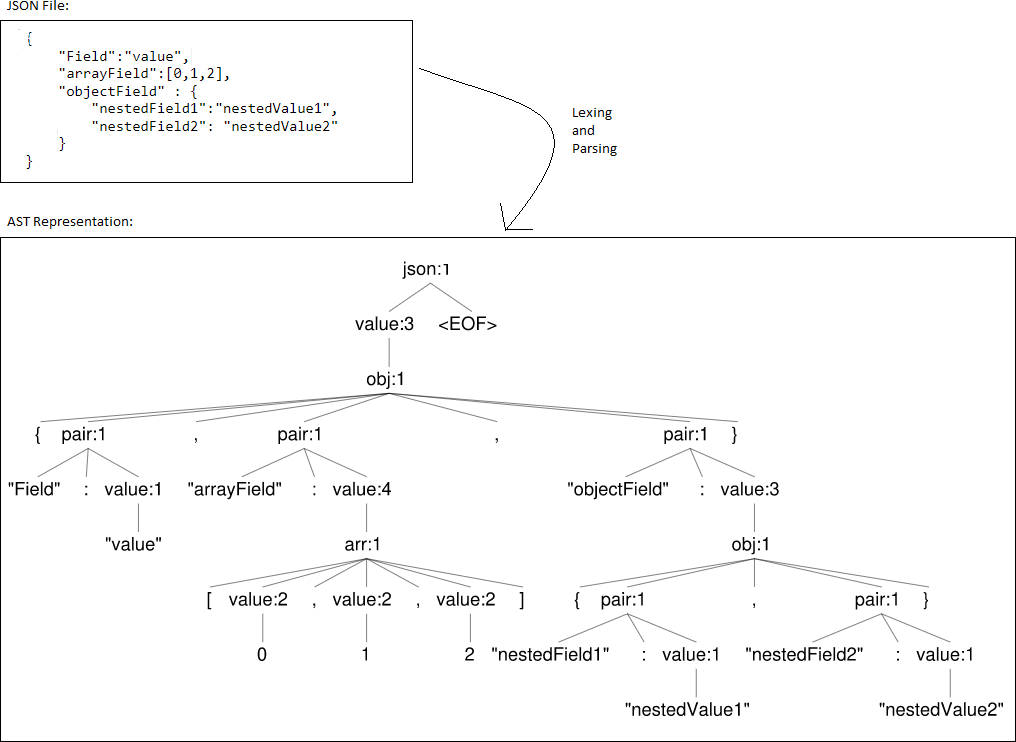
\includegraphics[width =1.2\textwidth]{dissertation/images/json file and AST.png}
%\end{center}
}


\pagebreak

\section{JSON grammar file}
%\addcontentsline{toc}{section}{JSON grammar file}
\label{appendix:grammar}
\begin{center}
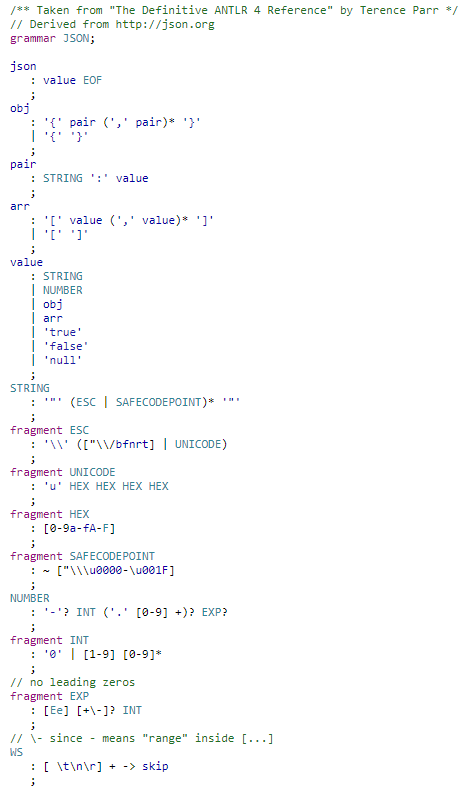
\includegraphics[width =0.9\textwidth]{dissertation/images/json grammar.png}
\end{center}

\pagebreak


\section{JSONTalk User Study}
%\addcontentsline{toc}{section}{JSONTalk User Study}
\label{appendix:study}
The following pages include a PDF version of the Qualtrics study we used for the evaluation of JSONTalk.
\centering
\includepdf[pages=-]{"images/JSONTalk user study"}

\section{Descriptions of JSON files generated by ChatGPT}
\label{appenidix:chatGPT}
\textbf{Description generated for file A:}

\noindent\fbox{
\small
    \parbox{\textwidth}{
        This is a JSON (JavaScript Object Notation) file, which is a lightweight data interchange format. The file contains an object with two key-value pairs.
        
        The first key is "store", which has a nested structure. Within "store", there are two key-value pairs. The first is "book", which is an array of four objects representing books. Each book object has properties such as "category", "author", "title", "isbn" (for some books), and "price".
        
        The second key within "store" is "bicycle", which is another object with properties "color" and "price".
        The second key-value pair in the JSON object is "expensive", which has a value of 10.
        
        Overall, this JSON file represents a simple inventory of a store that sells books and bicycles, with details on each item's category, author, title, ISBN (where applicable), color, and price.

    }
}
\textbf{Description generated for file B:}

\noindent\fbox{
\small
    \parbox{\textwidth}{
        The given code is a JSON file, which stands for JavaScript Object Notation. It is a lightweight format for storing and exchanging data between different systems. The JSON file contains a set of key-value pairs, where each key is a string and each value can be a string, number, boolean, array, or another JSON object.

        In this particular example, the JSON object has several key-value pairs:

        "name": "Jane Doe" - This key-value pair stores the name of the person as a string value.
        
        "email": "jane.doe@example.com" - This key-value pair stores the email address of the person as a string value.

        "address": {...} - This key-value pair stores an object that represents the address of the person. The address object itself contains several key-value pairs that store the street, city, state, and zip code as string values.

        "phoneNumbers": [...] - This key-value pair stores an array of objects that represent the person's phone numbers. Each object contains two key-value pairs, one for the type of number (home or work) and one for the phone number itself.

        "age": 35 - This key-value pair stores the age of the person as a number value.

        "isMarried": true - This key-value pair stores a boolean value that indicates whether the person is married or not.

        "hobbies": [...] - This key-value pair stores an array of strings that represent the person's hobbies.
    }
}

\textbf{Description generated for file C:}

\noindent\fbox{
\small
    \parbox{\textwidth}{
        This is a JSON (JavaScript Object Notation) file that contains data in a structured format. It consists of three main properties: "title", "description", and "items".
        
        The "title" property is a string that provides a title for the JSON file, and the "description" property is another string that provides a brief description of the   file.
        
        The "items" property is an array of objects, where each object represents a different item. Each item has three properties: "name", "quantity", and "price". The "name" property is a string that identifies the name of the item, the "quantity" property is an integer that represents the quantity of that item, and the "price" property is a number that represents the price of that item.
        
        In this example, there are three items listed: "item1", "item2", and "item3", each with their respective quantity and price values. This JSON file might be used to store and transmit data about items in a shopping cart, for example.

    }
}

\pagebreak


\addcontentsline{toc}{section}{Signed Ethics Checklist}
\label{appendix:ethics}
\centering
\includepdf[pages=-]{"images/Evaluation results/Signed Ethics Form.pdf"}

\end{appendices}

%==================================================================================================================================
%   BIBLIOGRAPHY   

% The bibliography style is abbrvnat
% The bibliography always appears last, after the appendices.

\bibliographystyle{abbrvnat}

\bibliography{l4proj}

\end{document}
